%\documentclass[serif, aspectratio=169]{beamer}  % for 16:9 ratio
\documentclass[serif]{beamer}  % for 4:3 ratio
\usepackage[T1]{fontenc} 
\usepackage{hyperref}
\usepackage{latexsym,amsmath,xcolor,multicol,booktabs,calligra}
\usepackage{graphicx,pstricks,listings,stackengine}
\usepackage{multimedia}

\author{
    Valeria De Stasio \\ 
    \and  
    Christian Faccio \\
    \and  
    Carlos Velázquez Fernández
}
\title{Detection and tracking of fishes: \\ an analysis of the YOLOv8 model}
\date{\small July 25, 2025}
\usepackage{UoWstyle}

% defs
\def\cmd#1{\texttt{\color{red}\footnotesize $\backslash$#1}}
\def\env#1{\texttt{\color{blue}\footnotesize #1}}
\definecolor{deepblue}{rgb}{0,0,0.5}
\definecolor{deepred}{RGB}{153,0,0}
\definecolor{deepgreen}{rgb}{0,0.5,0}
\definecolor{halfgray}{gray}{0.55}

\lstset{
    basicstyle=\ttfamily\tiny,
    keywordstyle=\bfseries\color{deepblue},
    emphstyle=\ttfamily\color{deepred},    % Custom highlighting style
    stringstyle=\color{deepgreen},
    numbers=left,
    numberstyle=\tiny\color{halfgray},
    rulesepcolor=\color{red!20!green!20!blue!20},
    frame=shadowbox,
}


\begin{document}

\begin{frame}
    \vfill
    \begin{center}
        
\includegraphics[keepaspectratio, scale=0.15]{images/logo.jpg}
        
        \vspace{1cm}
        
        \begin{beamercolorbox}[wd=\textwidth,center,rounded=true]{title}
            {\textbf{Detection, classification and tracking of fishes: \\ an analysis of the YOLOv8 model}}
        \end{beamercolorbox}
        
        \vspace{1cm}
        
        {July 25, 2025}
    \end{center}
    \vfill
\end{frame}

\begin{frame}    
\tableofcontents[sectionstyle=show,
subsectionstyle=show/shaded/hide,
subsubsectionstyle=show/shaded/hide]
\end{frame}

\section{Theory}

\begin{frame}
\frametitle{History of fish detection}
\centering
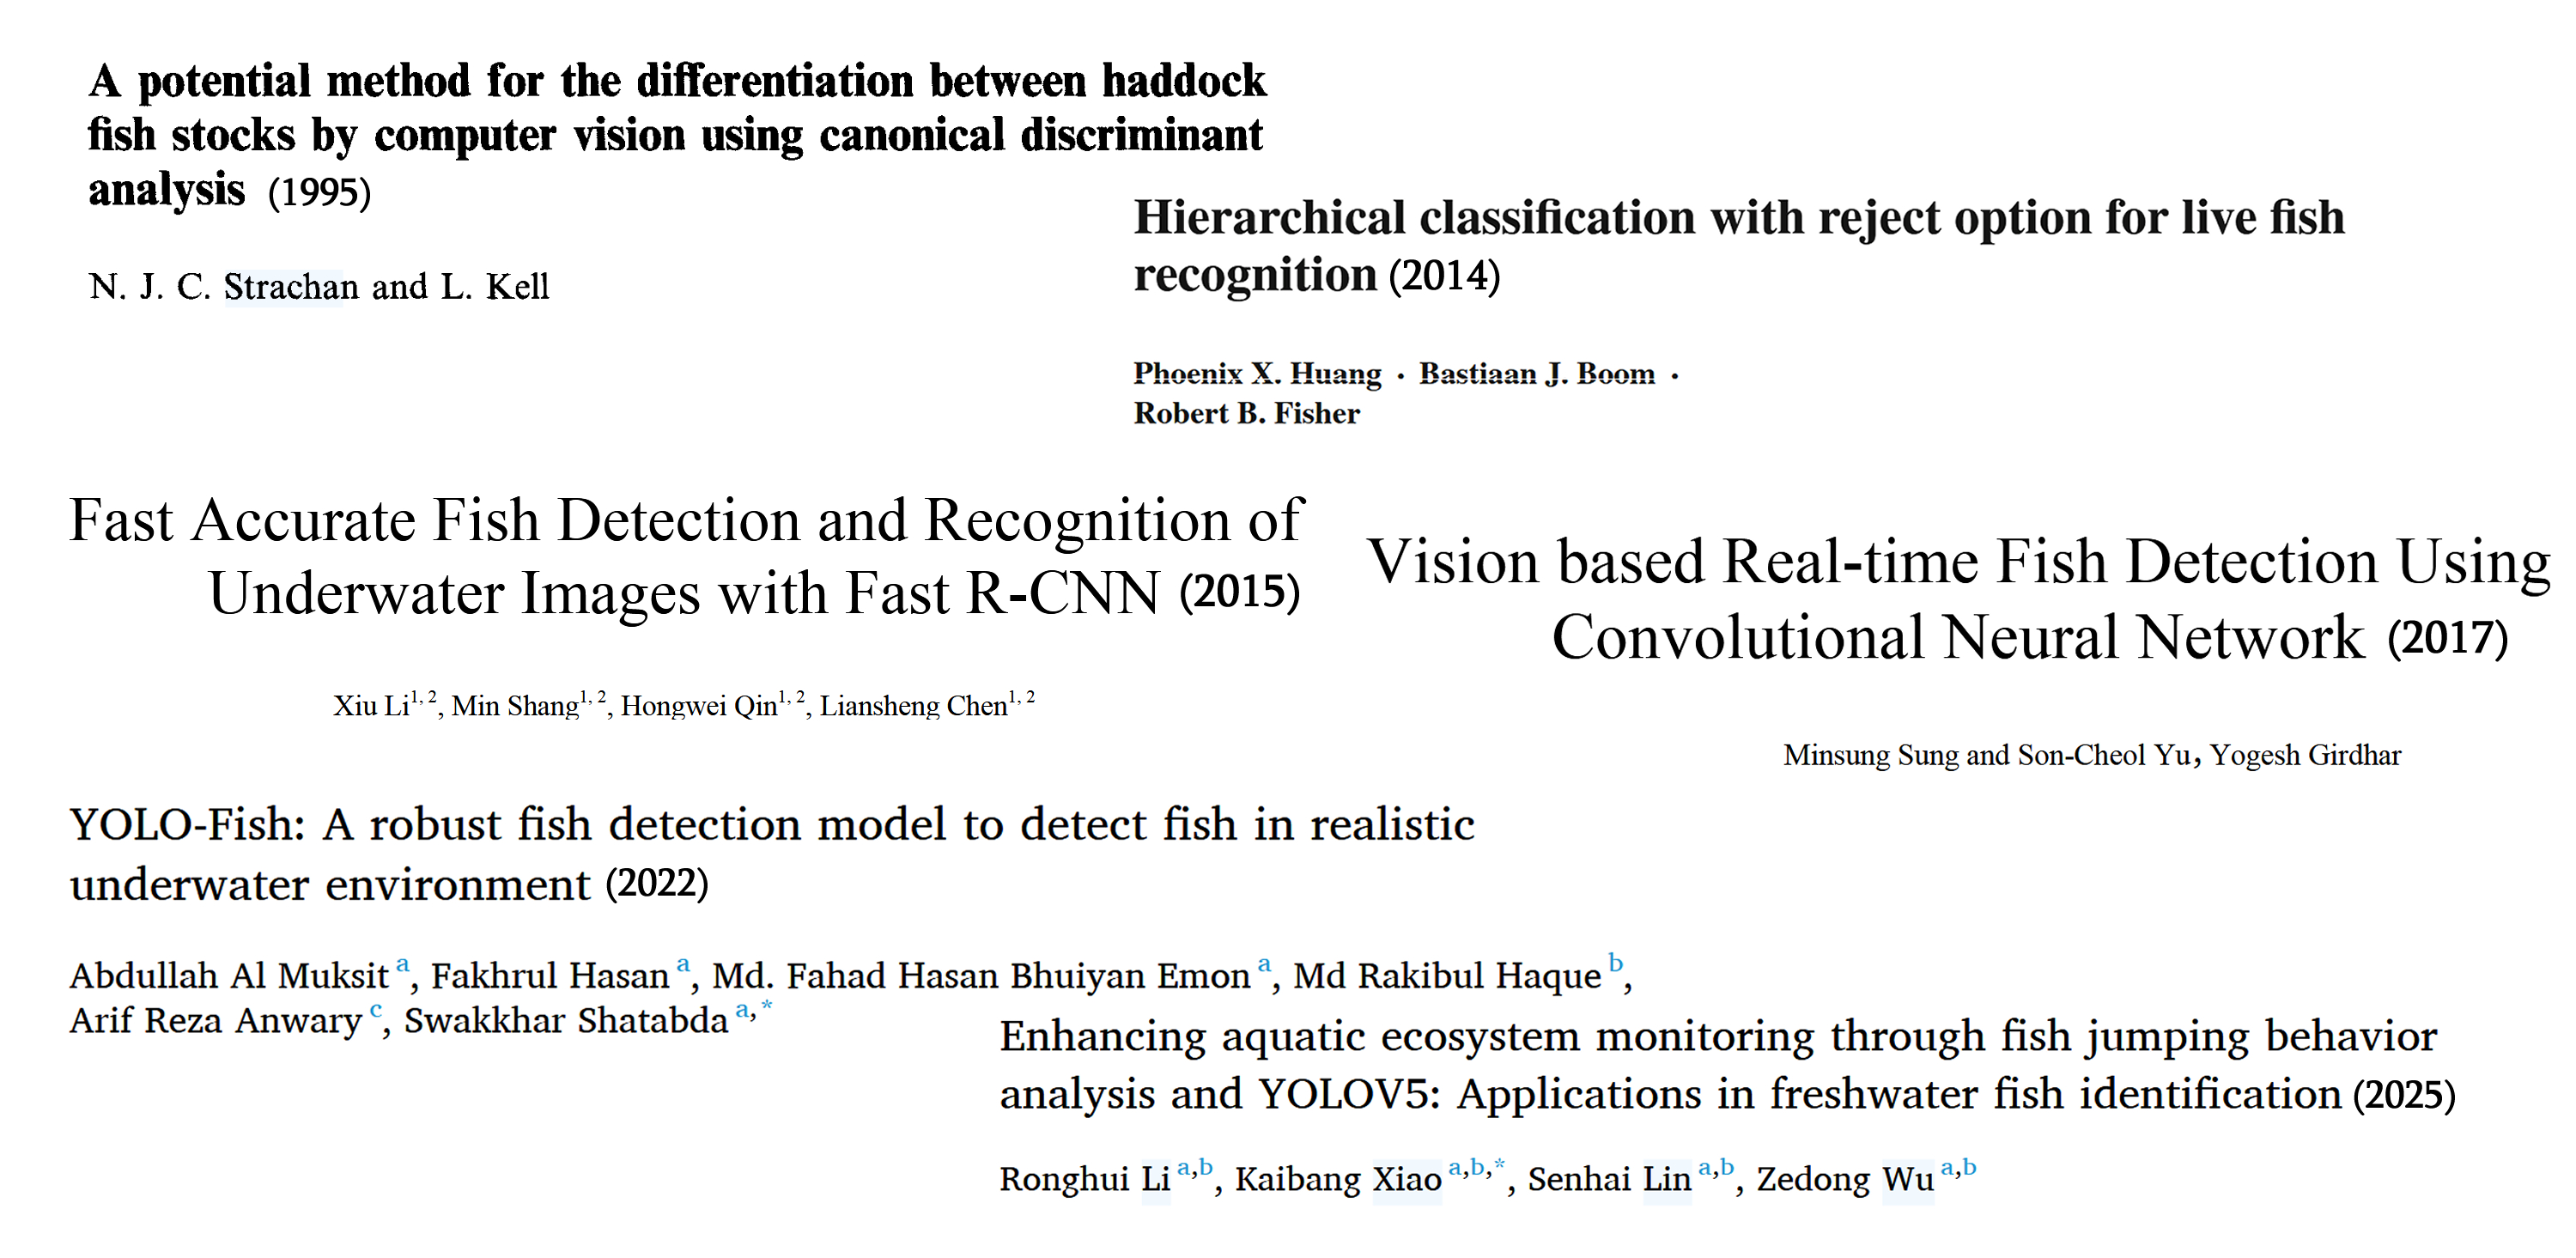
\includegraphics[width=1\linewidth]{images/Fish detection papers with years.jpg}
\end{frame}

\begin{frame}
\frametitle{10 years of YOLO}
\centering
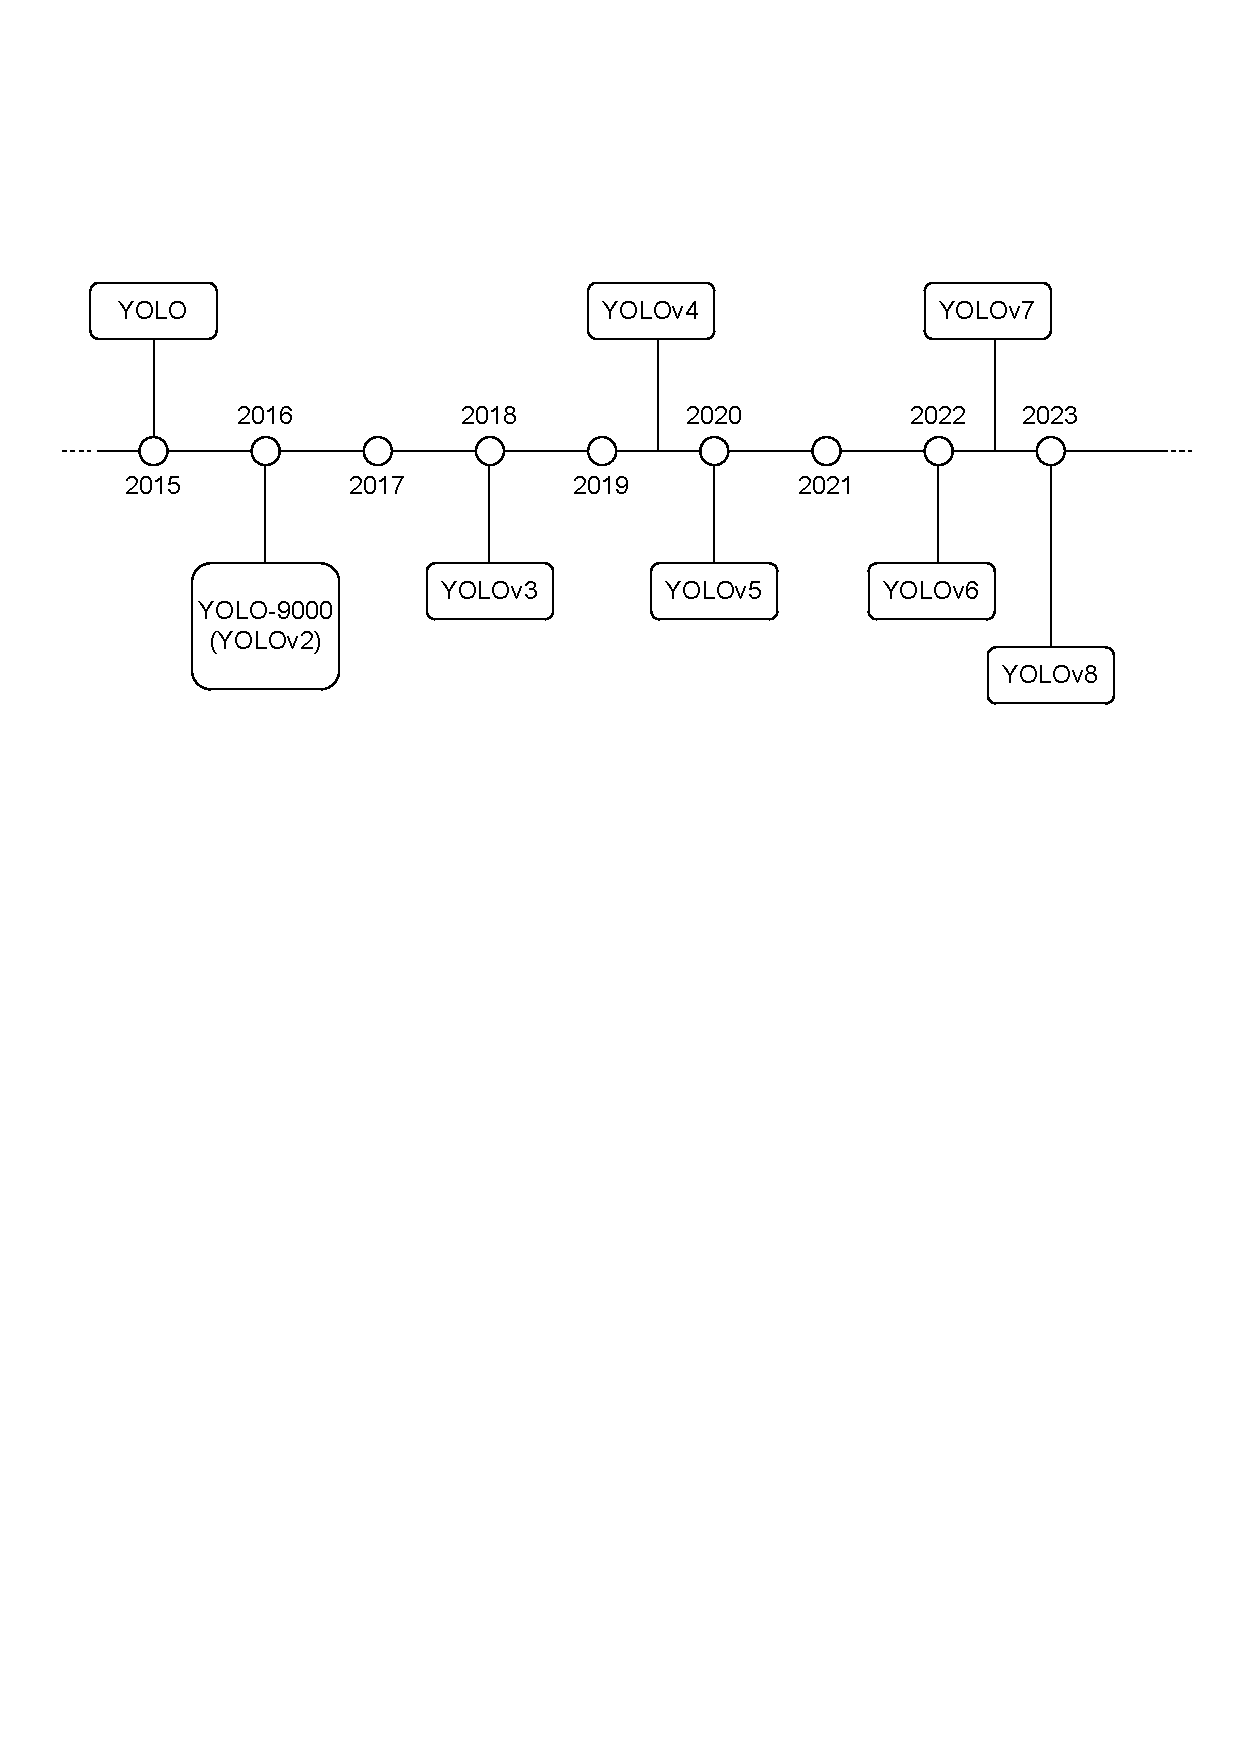
\includegraphics[width=1\linewidth,keepaspectratio]{images/yolo_timeline.pdf}
\end{frame}

\begin{frame}
\frametitle{YOLOv8}
\centering
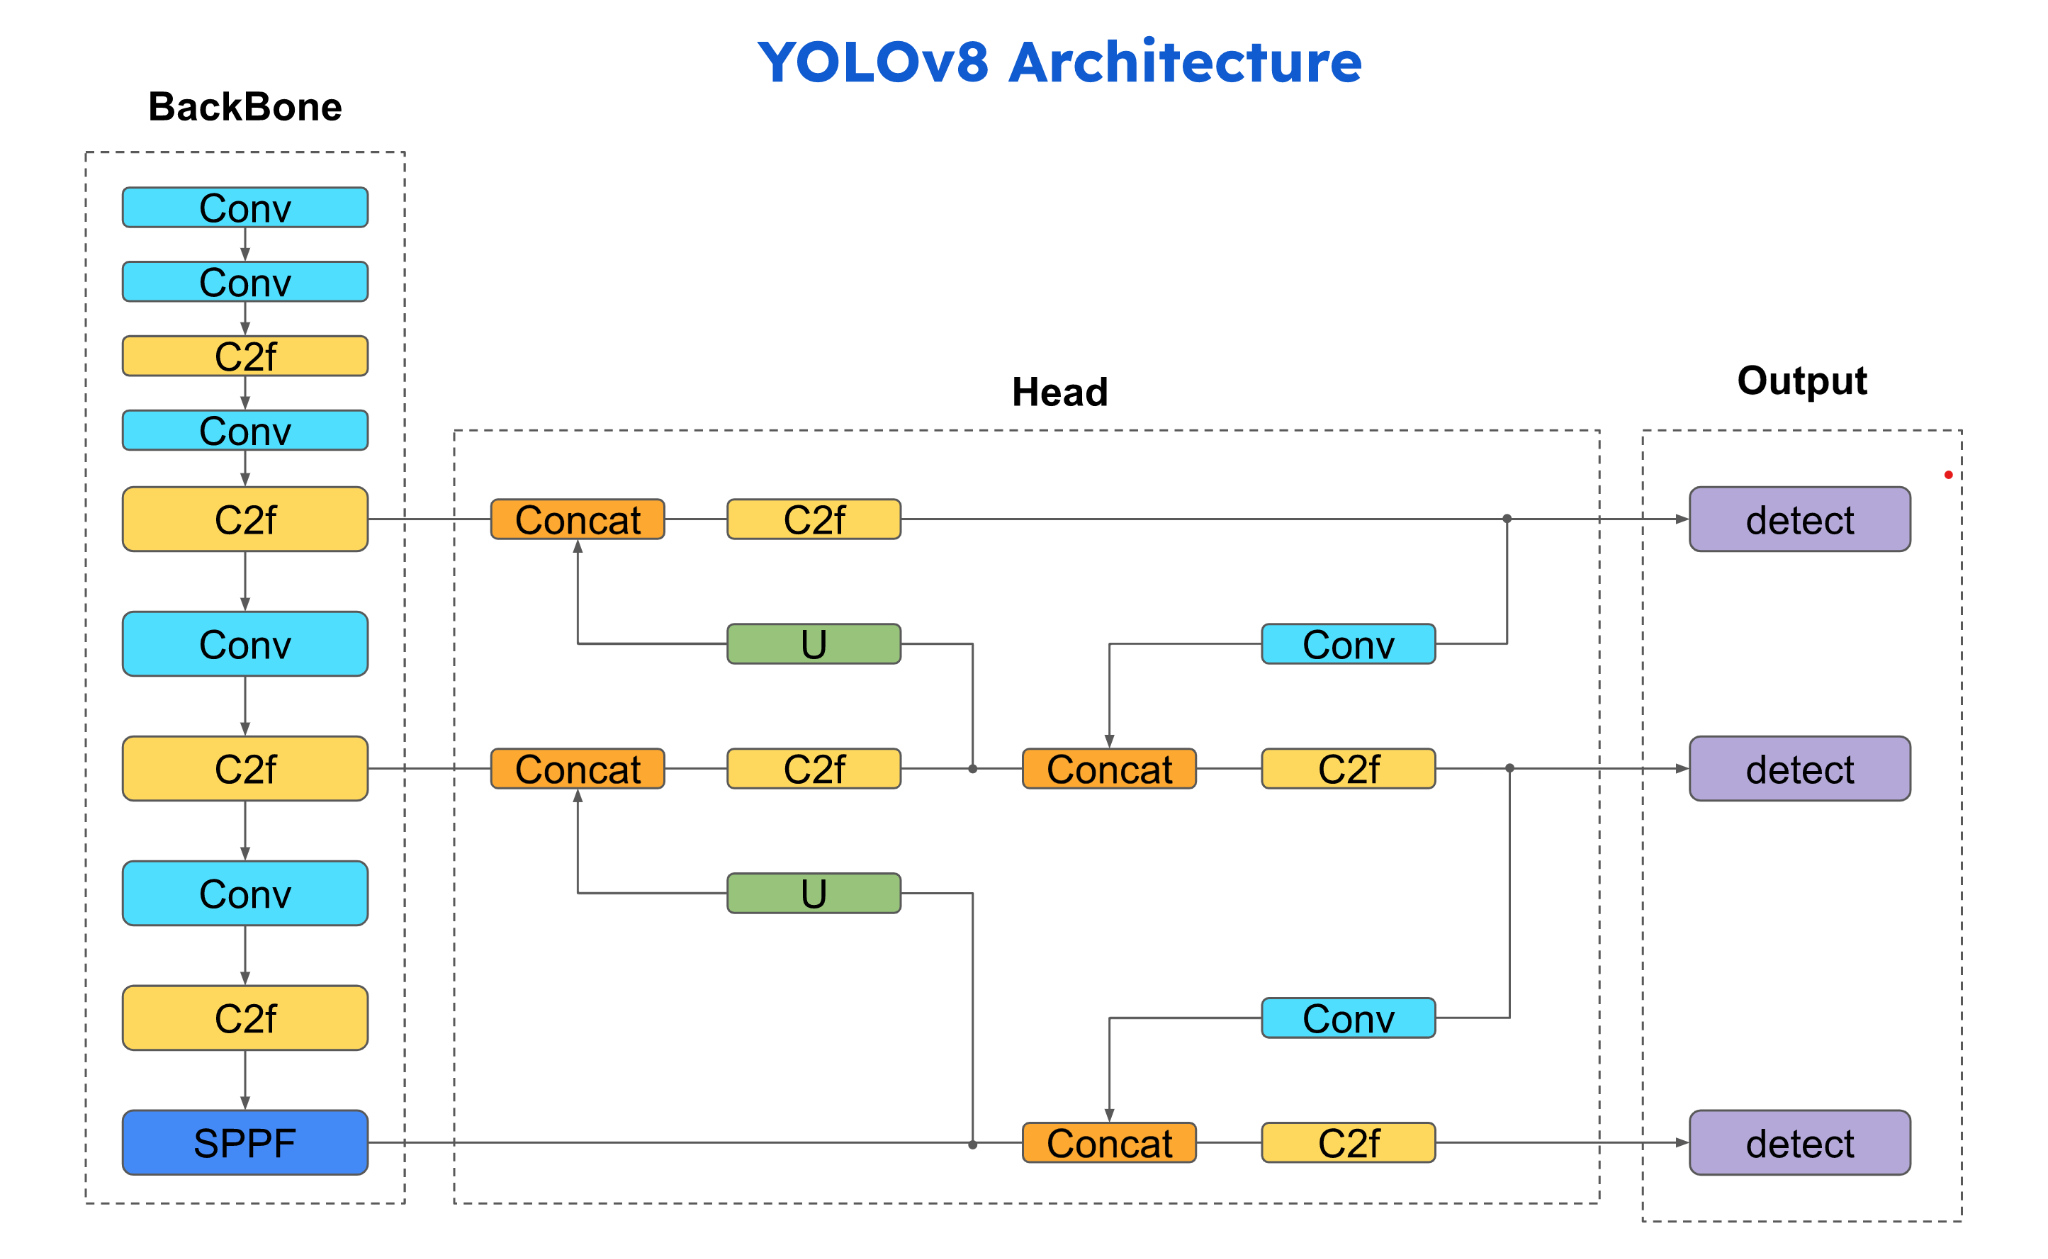
\includegraphics[width=1\linewidth]{images/YOLO_architecture_simple.png}
\footnote{\cite{sohan2024review}}
\end{frame}

\begin{frame}
\frametitle{Complete Architecture}
\centering
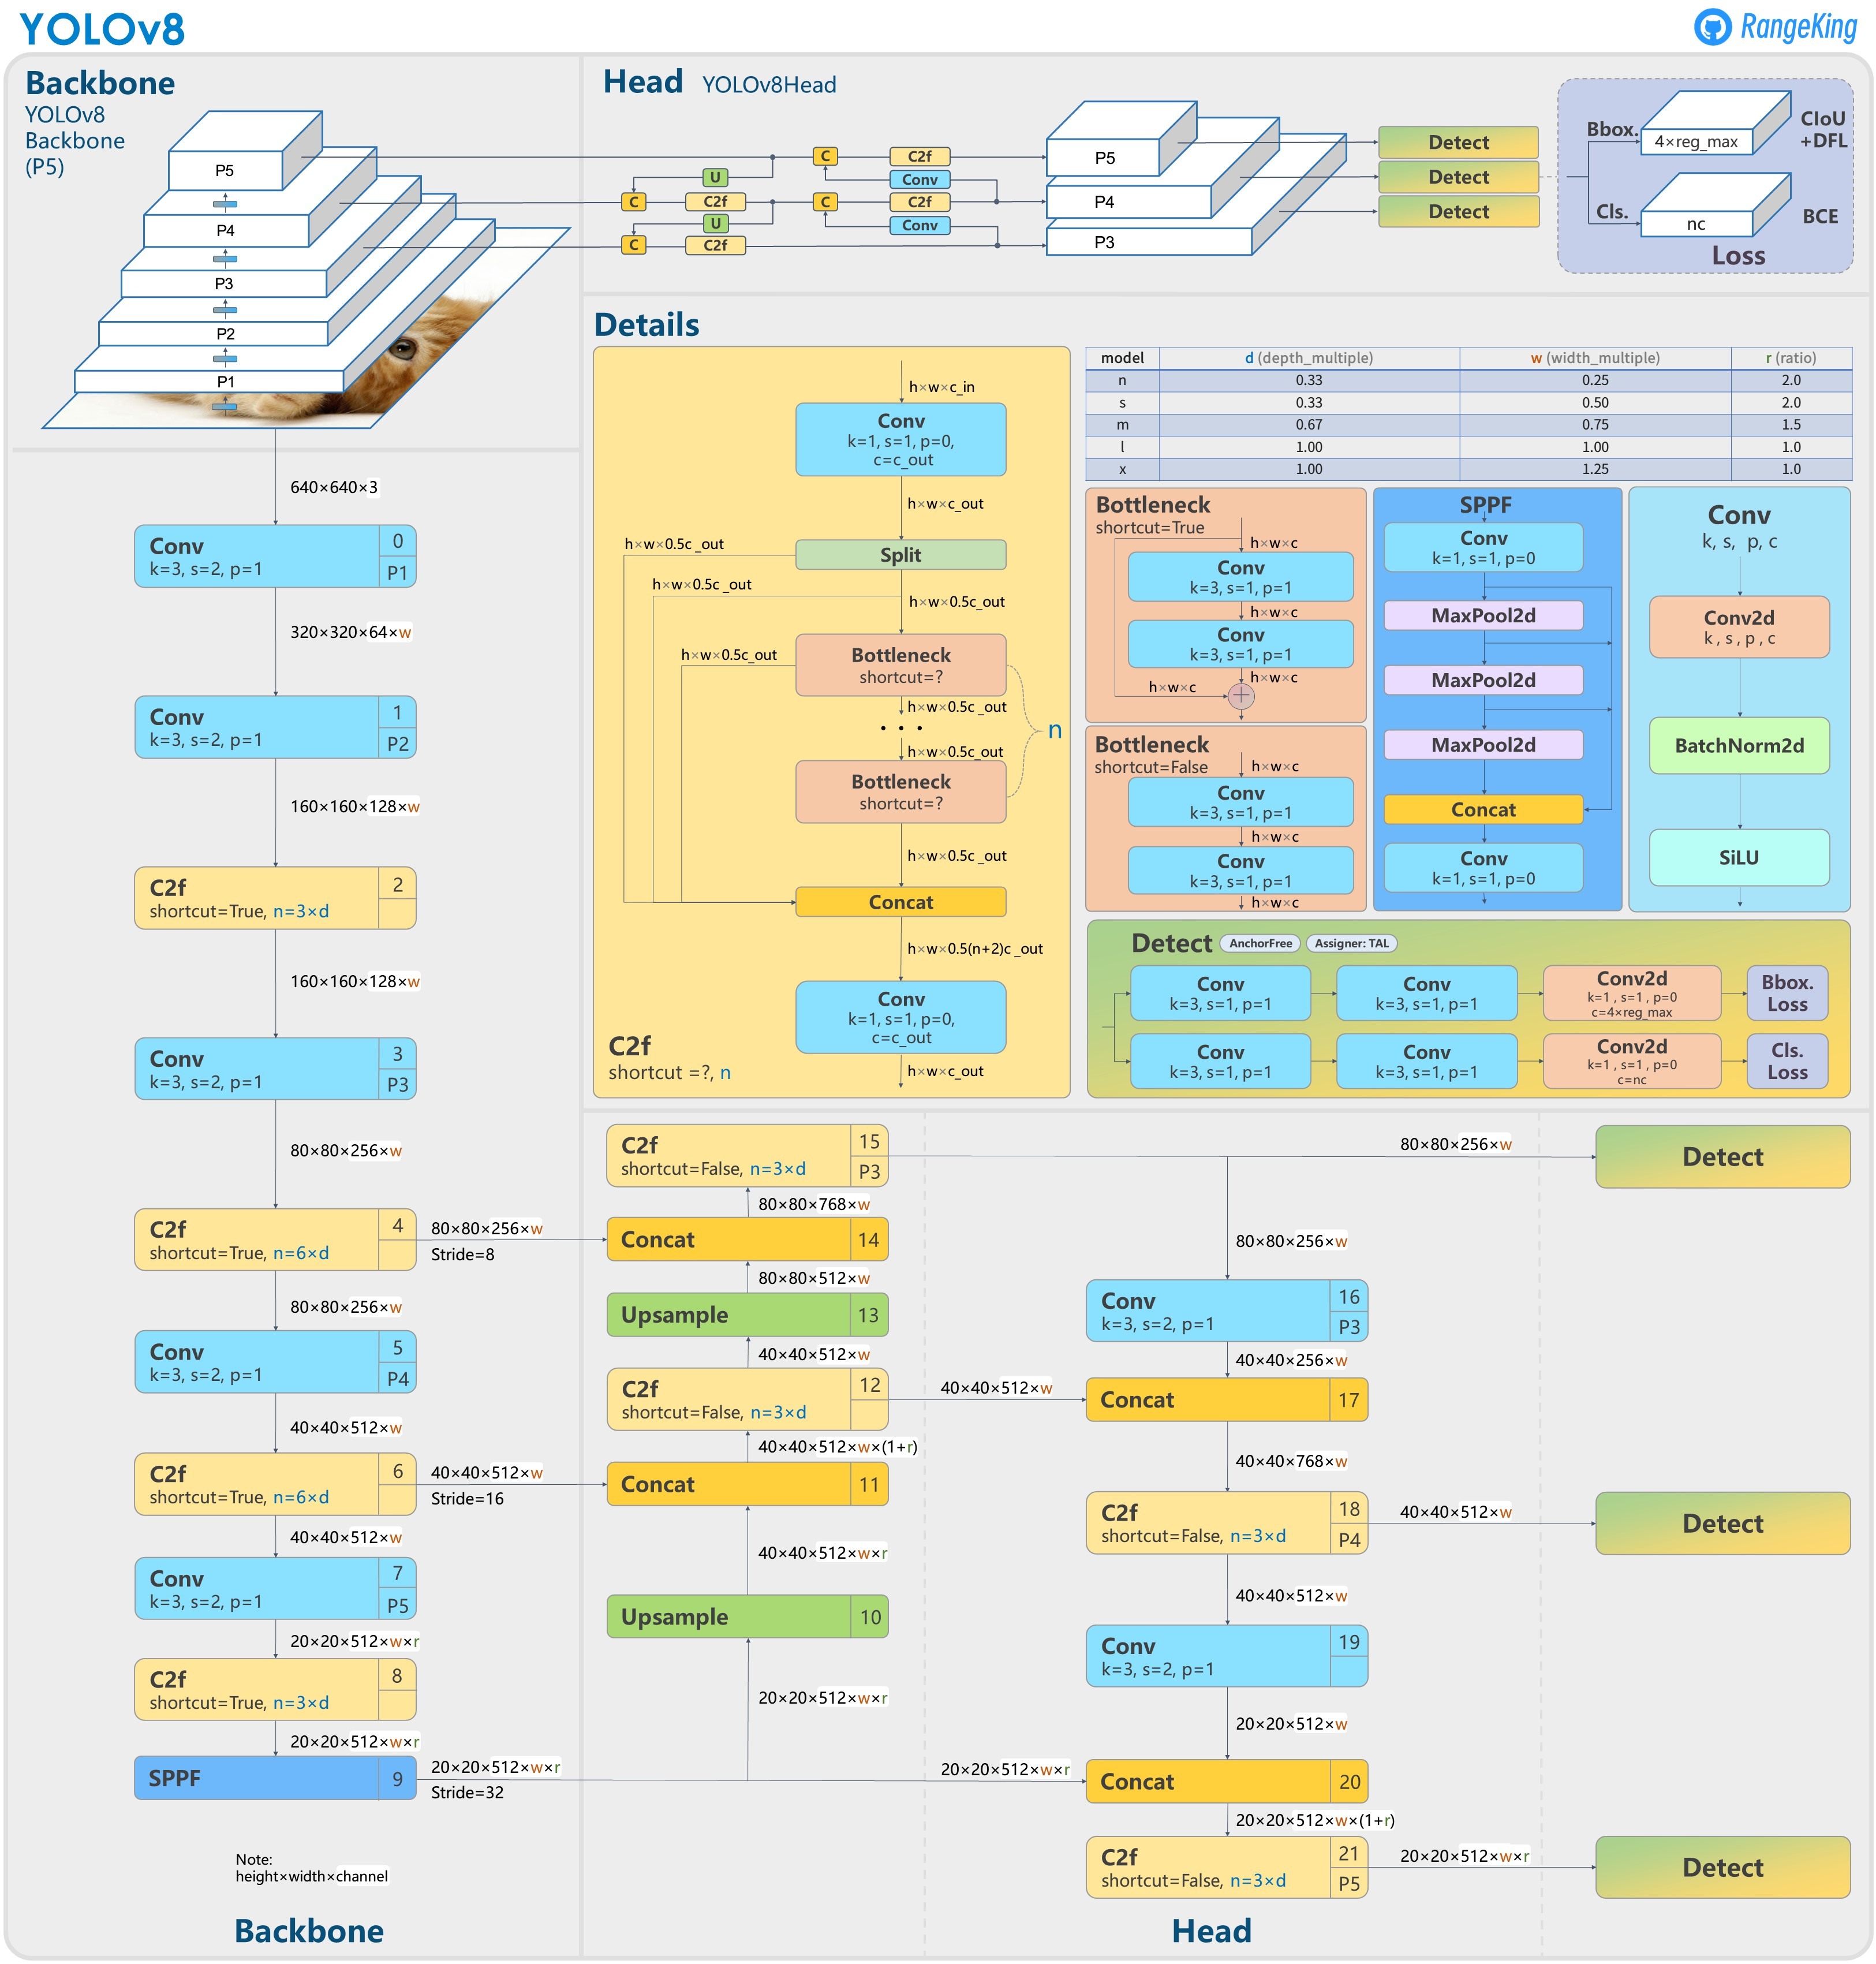
\includegraphics[height=0.85\textheight,keepaspectratio]{images/YOLO_architecture.jpg}
\footnote{\cite{rangeking2023yolov8}}
\end{frame}

\begin{frame}
\frametitle{Modules}
\centering
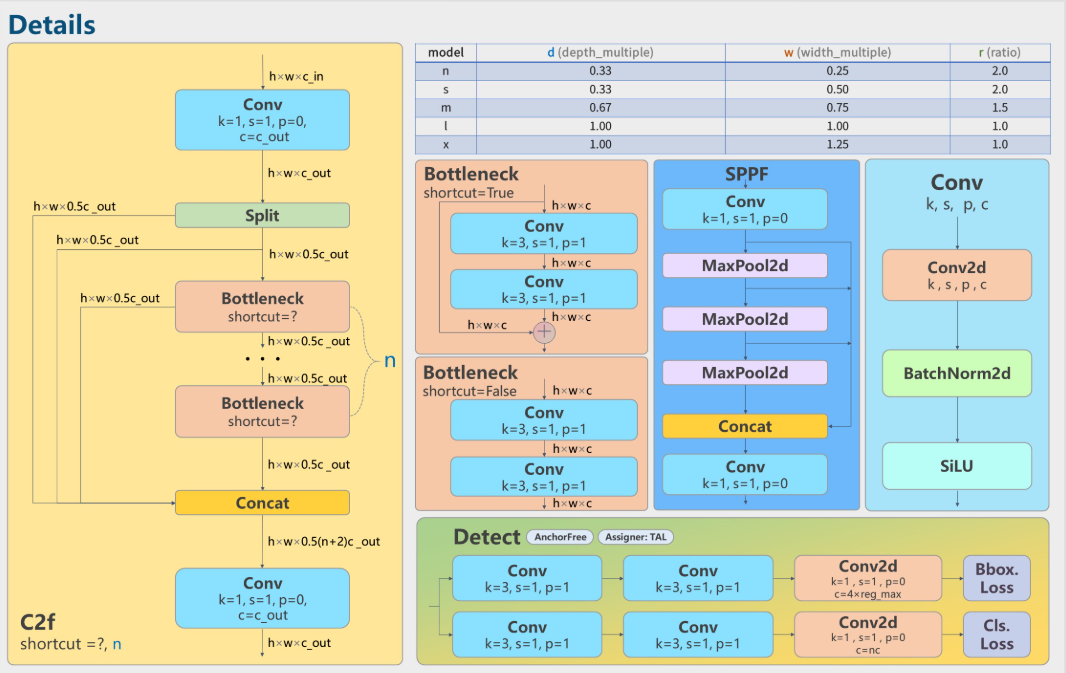
\includegraphics[width=1\linewidth,keepaspectratio]{images/module_details.png}
\end{frame}

\section{Detection}

\begin{frame}
\frametitle{Datasets}
\begin{columns}
\begin{column}{0.5\textwidth}
	\centering
	\textbf{DeepFish  --> }\\
\end{column}

\begin{column}{0.5\textwidth}
	\centering
	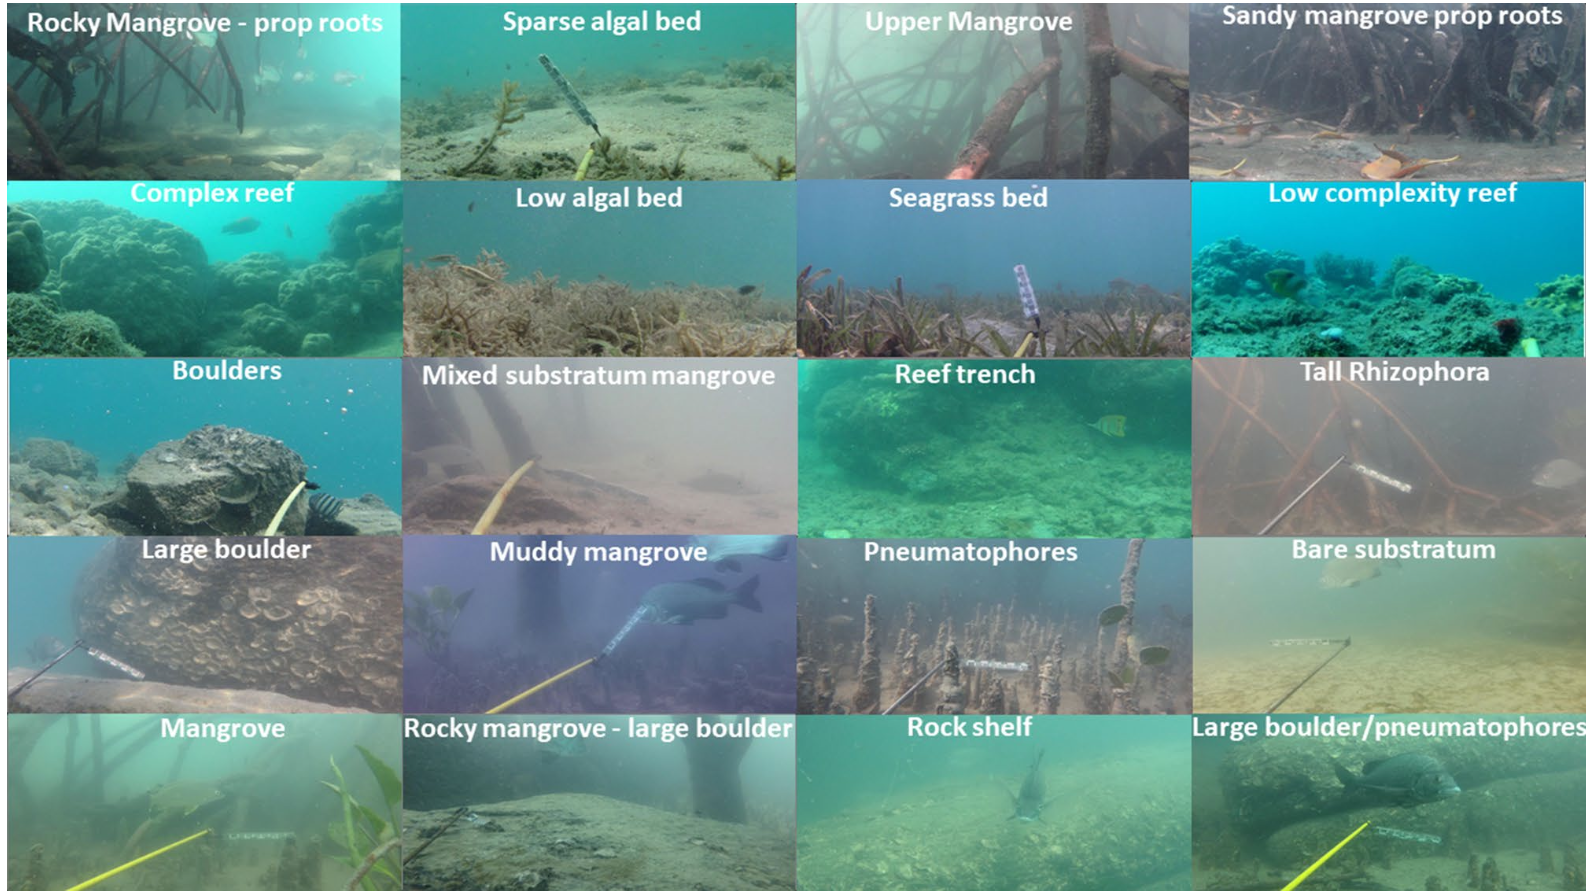
\includegraphics[width=0.95\textwidth]{images/deepfish.png}
\end{column}
\end{columns}

\vspace{1cm}

\begin{columns}
\begin{column}{0.5\textwidth}
	\centering
	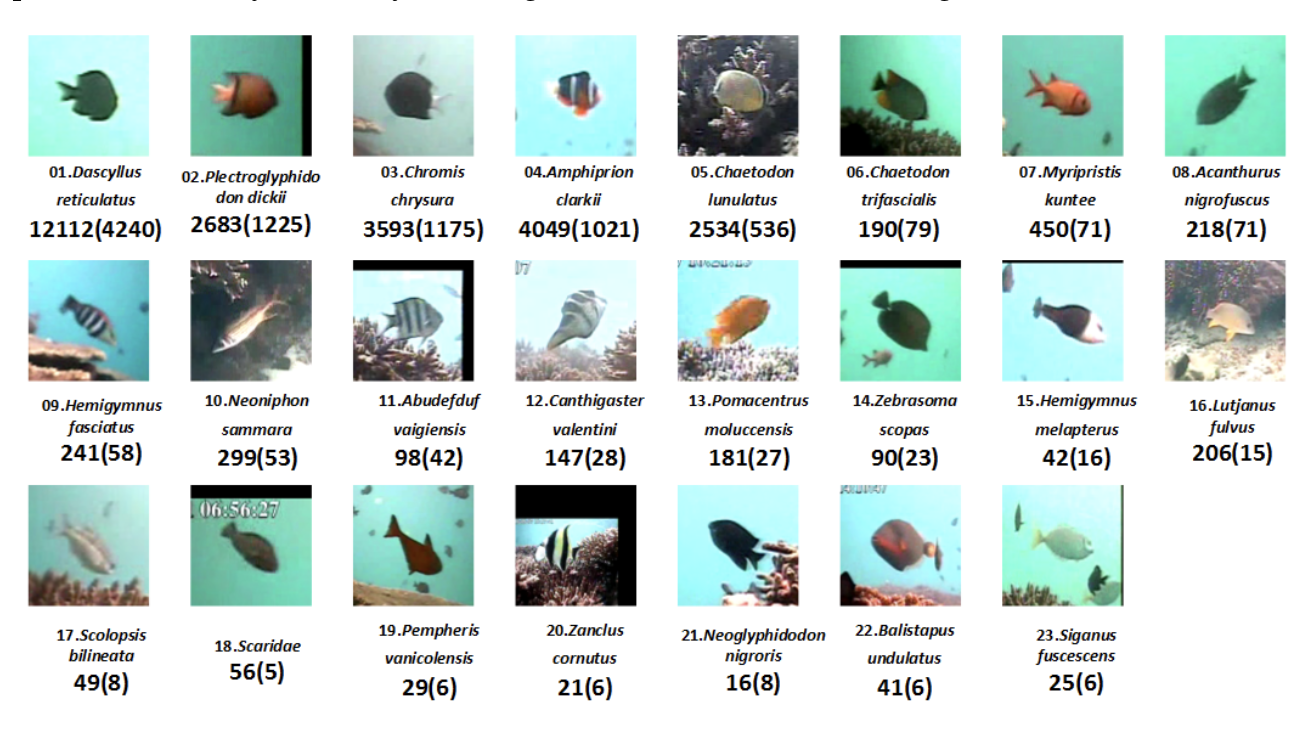
\includegraphics[width=0.95\textwidth]{images/f4k.png}	
\end{column}

\begin{column}{0.5\textwidth}
	\centering
	\textbf{<--  Fish4Knowledge}
\end{column}
\end{columns}
\end{frame}

\begin{frame}[fragile]
\frametitle{Datasets structure}
\begin{columns}
\begin{column}{0.3\textwidth}
\centering
\textbf{DeepFish}
\begin{lstlisting}[language=python]
.
├── 7117
│   ├── train
│   └── valid
├── 7268
├── 7393
├── 7398
├── 7426
├── 7434
├── 7463
├── 7482
├── 7490
├── 7585
├── 7623
├── 9852
├── 9862
├── 9866
├── 9870
├── 9892
├── 9894
├── 9898
├── 9907
├── 9908
├── classes.txt
├── Nagative_samples
└── test
\end{lstlisting}
\end{column}

\begin{column}{0.3\textwidth}
\centering
\textbf{Fish4Knowledge}
\begin{lstlisting}[language=python]
.    
┣ fish_image
┃ ┣ fish_01
┃ ┃ ┣ fish_x.png
┃ ┃ ┗ ...
┣ gt_bounding_boxes
┃ ┣ gt_106.xml
┃ ┗ ...
┣ mask_image
┃ ┣ mask_01
┃ ┃ ┣ mask_x.png
┃ ┃ ┗ ...
┗ videos
    ┣ gt_106.mp4
    ┗ ...

\end{lstlisting}
\end{column}

\begin{column}{0.3\textwidth}
\centering
\textbf{YOLO format}
\begin{lstlisting}[language=python]
.
├── data.yaml
├── test
│   ├── images
│   └── labels
├── train
│   ├── images
│   └── labels
└── val
    ├── images
    └── labels
\end{lstlisting}
\end{column}
\end{columns}
\end{frame}

\begin{frame}[fragile]
\frametitle{Configuration files (data.yaml)}
\begin{columns}
\begin{column}{0.45\textwidth}
\begin{lstlisting}[language=python]
train: path_to_train/images
val: path_to_val/images
test: path_to_test/images

nc: 1
names: ['Fish']
\end{lstlisting}
\end{column}

\begin{column}{0.45\textwidth}
\begin{lstlisting}[language=python]
train: path_to_train/images
val: path_to_val/images
test: path_to_test/images

nc: 23
names: [
  'Caranx_sexfasciatus',
  'F1', 
  'F2',
  'F3', 
  'F4',
  'F5',
  'F6',
  'F7',
  'Acanthopagrus_palmaris',
  'Lutjanus_russellii',
  'acanthopagrus_and_caranx',
  'acanthopagrus_palmaris', 
  'Gerres',
  'Caranx',
  'Amniataba_caudivittatus',
  'gerres_2',
  'gerres',
  'Epinephelus',
  'Fish',
  'juvenile',
  'palmaris',
  'EJP',
  'caudivittatus'
]
\end{lstlisting}
\end{column}
\end{columns}
\end{frame}

\begin{frame}
\frametitle{YOLOv8 models}
\begin{center}
\resizebox{\textwidth}{!}{%
\begin{tabular}{|l|c|c|c|c|c|c|}
\hline
\textbf{Model} & \textbf{size} & \textbf{mAP$^{\text{val}}$} & \textbf{Speed} & \textbf{Speed} & \textbf{params} & \textbf{FLOPs} \\
 & \textbf{(pixels)} & \textbf{50-95} & \textbf{CPU ONNX} & \textbf{A100 TensorRT} & \textbf{(M)} & \textbf{(B)} \\
 &  &  & \textbf{(ms)} & \textbf{(ms)} &  &  \\
\hline
YOLOv8n & 640 & 37.3 & 80.4 & 0.99 & 3.2 & 8.7 \\
\hline
YOLOv8s & 640 & 44.9 & 128.4 & 1.20 & 11.2 & 28.6 \\
\hline
YOLOv8m & 640 & 50.2 & 234.7 & 1.83 & 25.9 & 78.9 \\
\hline
YOLOv8l & 640 & 52.9 & 375.2 & 2.39 & 43.7 & 165.2 \\
\hline
YOLOv8x & 640 & 53.9 & 479.1 & 3.53 & 68.2 & 257.8 \\
\hline
\end{tabular}%
}
\end{center}
\end{frame}

\begin{frame}
\frametitle{General Parameters}
\begin{center}
\small
\begin{tabular}{|l|c|p{5.5cm}|}
\hline
\textbf{Parameter} & \textbf{Value} & \textbf{Description} \\
\hline
Epochs & 50-100 & Number of training iterations \\
\hline
Batch Size & 16 & Images processed simultaneously \\
\hline
Image Size & 640 & Input image resolution (pixels) \\
\hline
Optimizer & AdamW & Adaptive moment estimation with weight decay \\
\hline
Learning Rate & 0.001 & Initial learning rate with cosine scheduling \\
\hline
Weight Decay & 0.0005 & L2 regularization strength \\
\hline
patience & 10 & Epochs to wait before early stopping \\
\hline
Warmup epochs & 3 & Gradual learning rate increase at start \\
\hline
cos\_lr & True & Cosine learning rate scheduler \\
\hline
close\_mosaic & 10 & Disable mosaic augmentation in last N epochs \\
\hline
\end{tabular}
\end{center}
\end{frame}


\begin{frame}
\frametitle{Specific Parameters (single-class vs multi-class)}
\begin{center}
\small
\begin{tabular}{|l|c|c|p{4cm}|}
\hline
    \textbf{Parameter} & \textbf{Single-class} & \textbf{Multi-class} & \textbf{Description} \\
\hline
cls & 0.5 & 1.0 & Weight affecting importance of correct class prediction\\
\hline
box & 7.5 & 7.5 & Weight influencing emphasis on accurately predicting bounding box coordinates\\
\hline
dfl & 1.5 & 1.5 & Weight used for fine-grained classification\\
\hline
mixup & 0.0 & 0.15 & Blends two images and their labels, creating composite image\\
\hline
copy\_paste & 0.1 & 0.3 & Copies and pastes objects across images to increase object instances\\
\hline
\end{tabular}
\end{center}
\end{frame}

\begin{frame}
\frametitle{AdamW}
$$
\phi_{t+1} \leftarrow \phi_t - \alpha \cdot (\frac{m_t}{v_t + \epsilon} + \lambda \phi_t)
$$
\vspace{0.5cm}
Where:
\begin{itemize}
	\item $m_t \leftarrow \frac{\beta_1 \cdot m_{t-1} + (1-\beta_1)g_t}{1 - \beta_1^t}$
	\item $v_t \leftarrow \frac{\beta_2 \cdot v_{t-1} + (1-\beta_2)g_t^2}{1 - \beta_2^t}$
	\item $g_t \leftarrow \nabla L_t(\phi_{t-1}) \quad  \mathbf{ (no  }\lambda \phi_{t-1} \mathbf{  here!)}$
\end{itemize}
\end{frame}

\begin{frame}
\frametitle{Loss Function}
$$
L_{yolov8} = \theta_{cls}\cdot L_{cls} + \theta_{box}\cdot L_{box} + \theta_{dfl}\cdot L_{dfl} 
$$
\begin{itemize}
	\item \textbf{Classification loss:} whether the model correctly identifies what type of fish (or object) it is.
	\item \textbf{Box loss:} how well the predicted bounding box overlaps with the ground truth box.
	\item \textbf{DFL:} Distributed Focal Loss, boosts performance by distributing the loss function across different object scales and classes.
\end{itemize}
\end{frame}

\begin{frame}
\frametitle{Training}
\centering
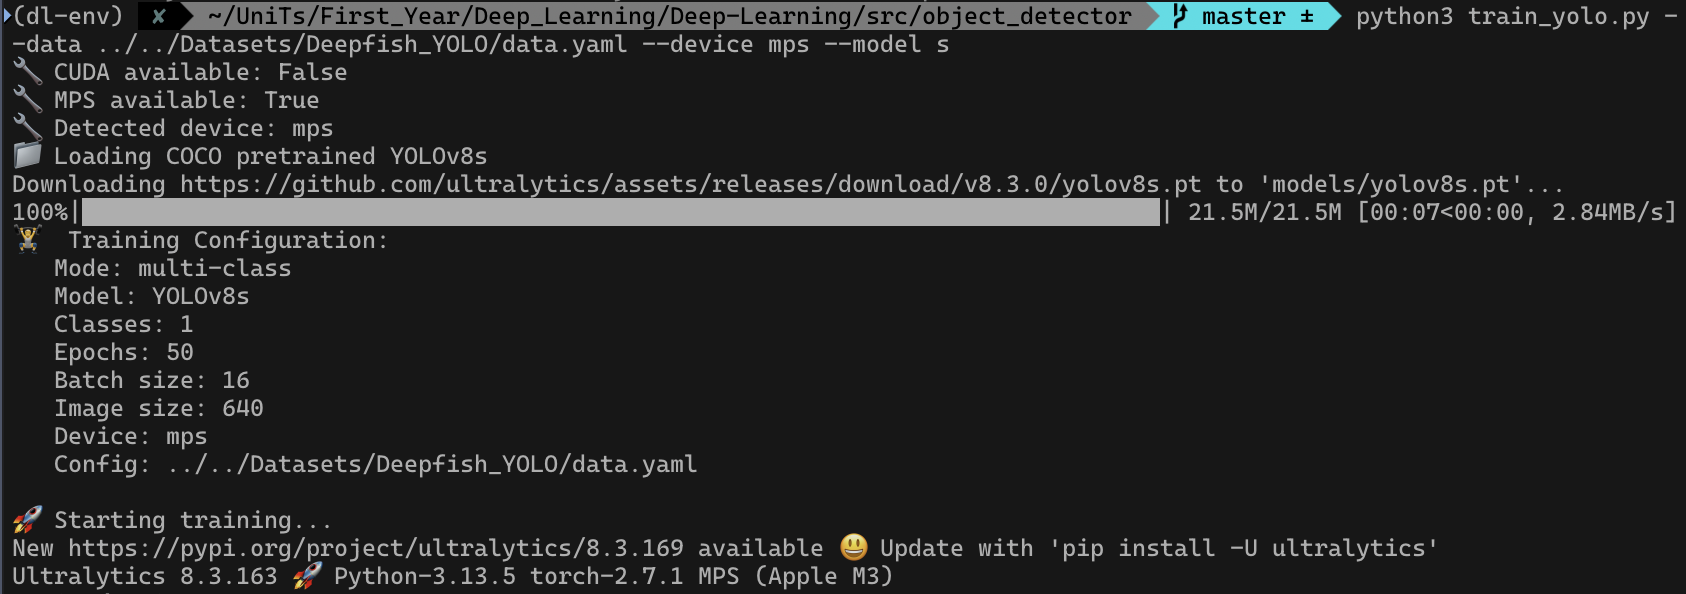
\includegraphics[width=0.7\textwidth]{images/training1.png}
\vspace{0.5cm}
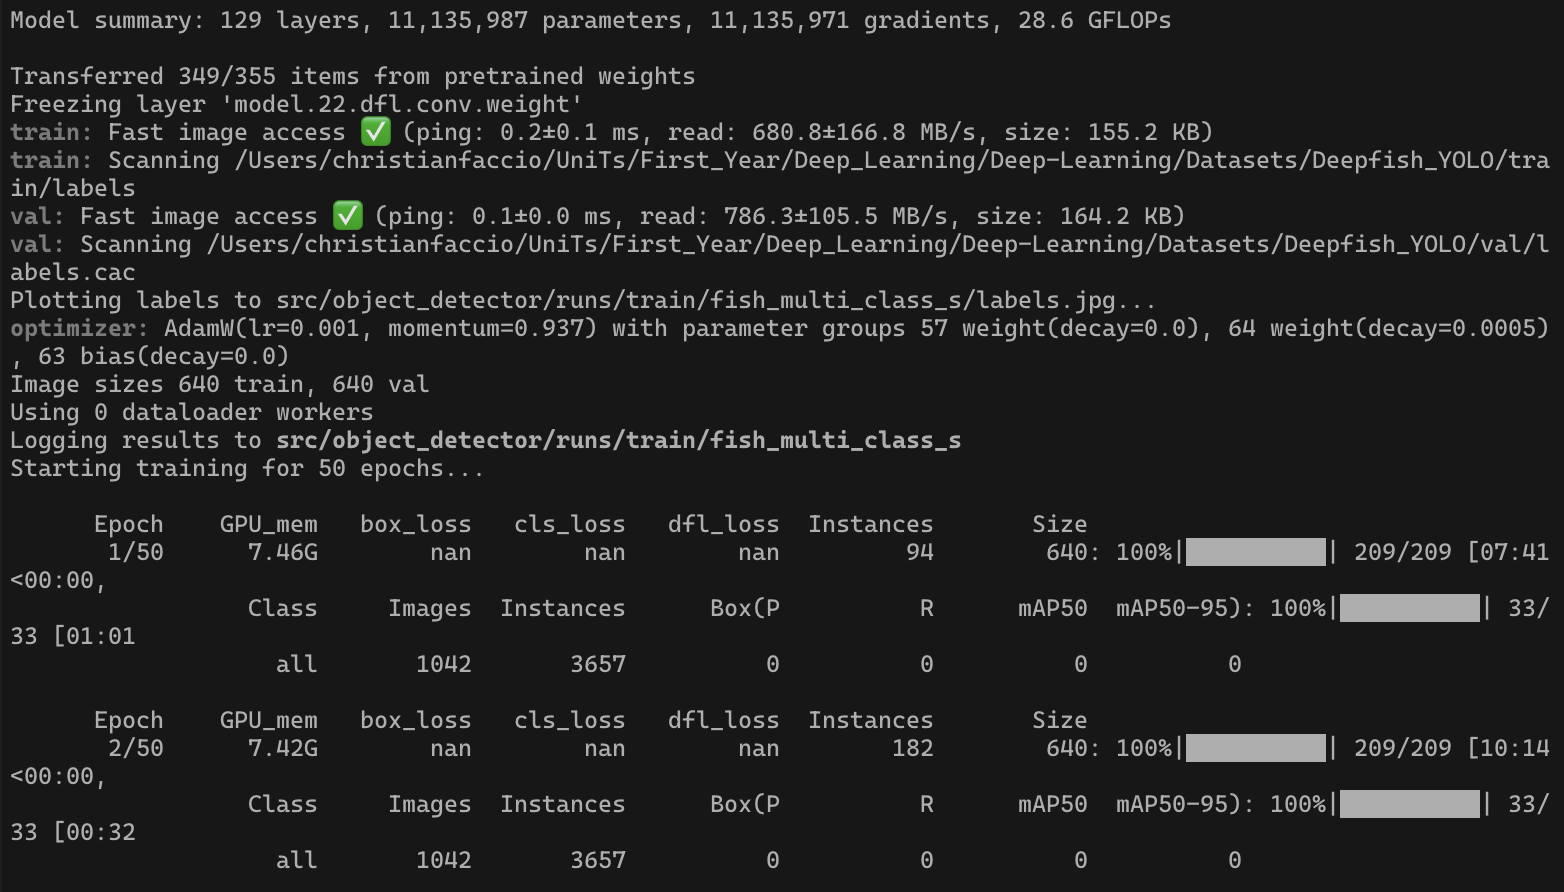
\includegraphics[width=0.7\textwidth]{images/training2.png}
\end{frame}

\begin{frame}
\centering
\textbf{Mixup feature}
\begin{columns}
\begin{column}{0.5\textwidth}
	\centering
	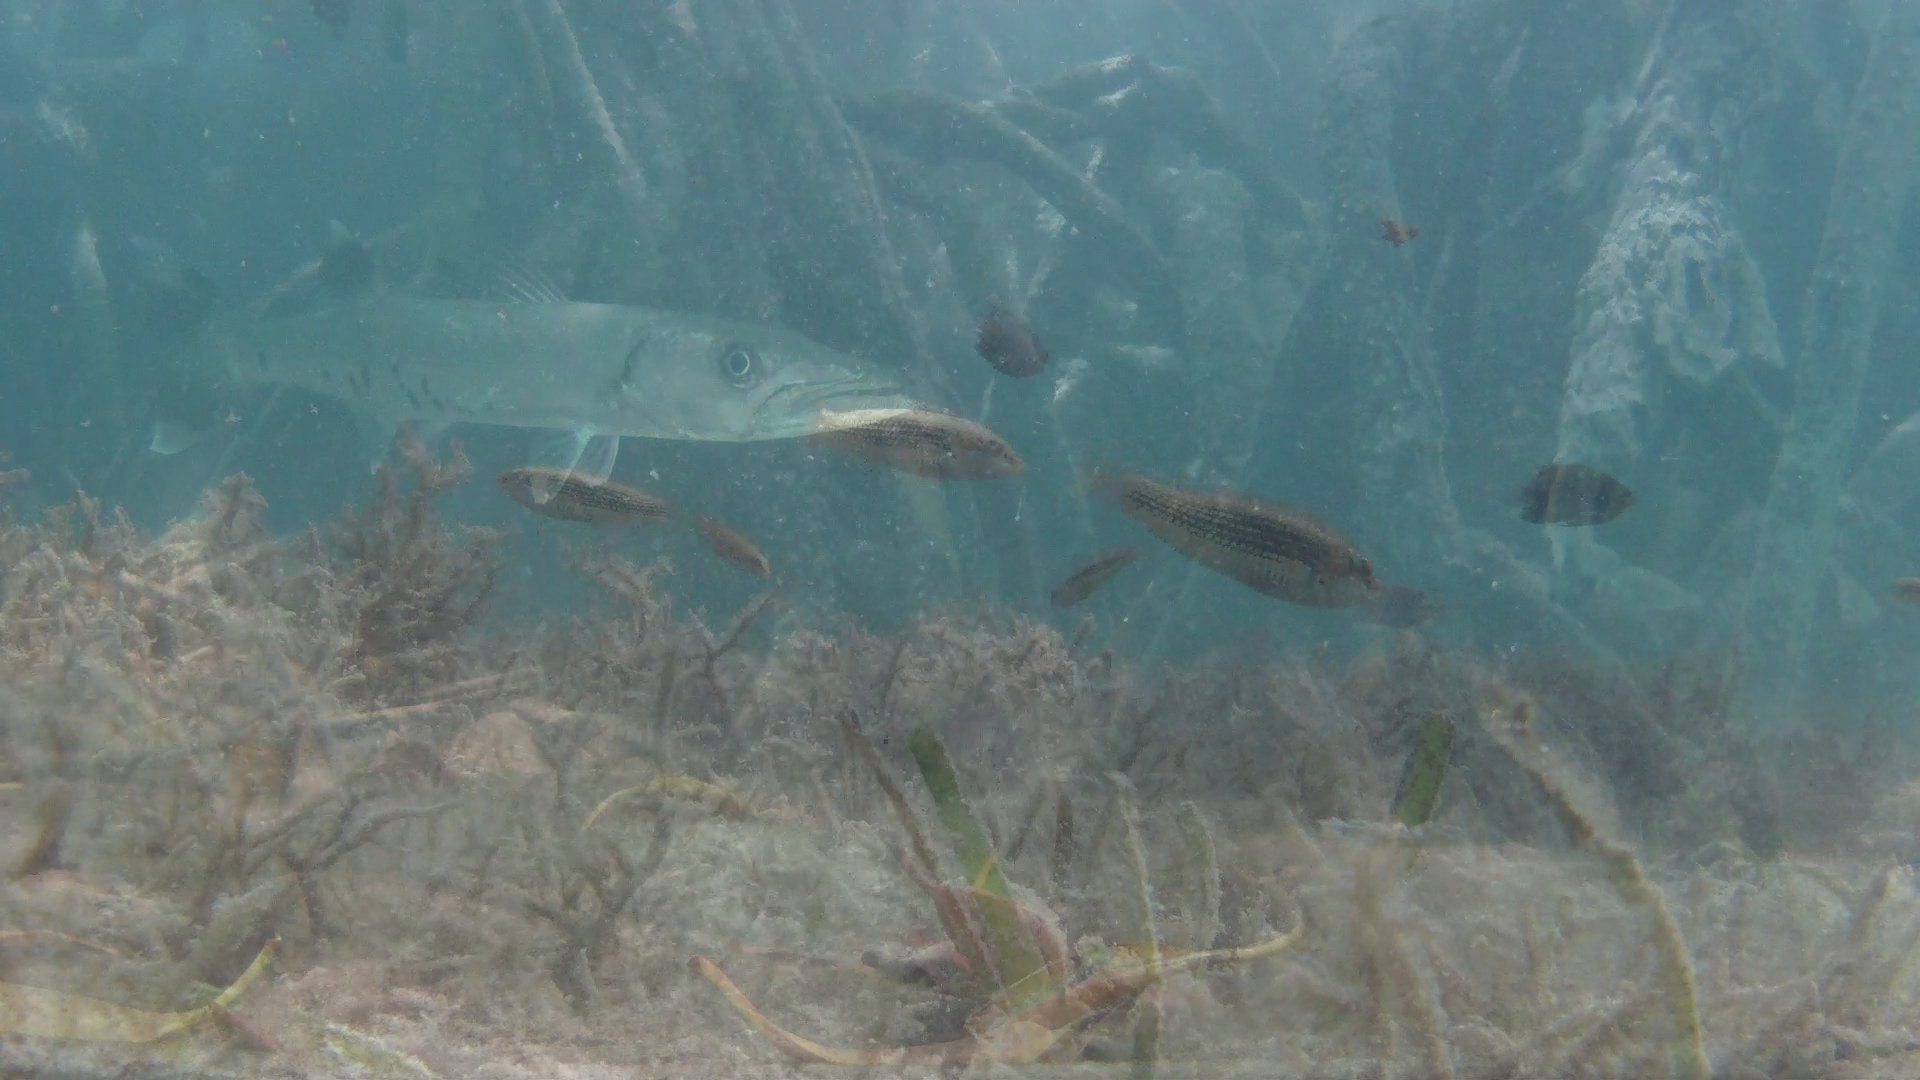
\includegraphics[width=0.8\textwidth]{images/mixup_1.jpg}
\end{column}

\begin{column}{0.5\textwidth}
	\centering
	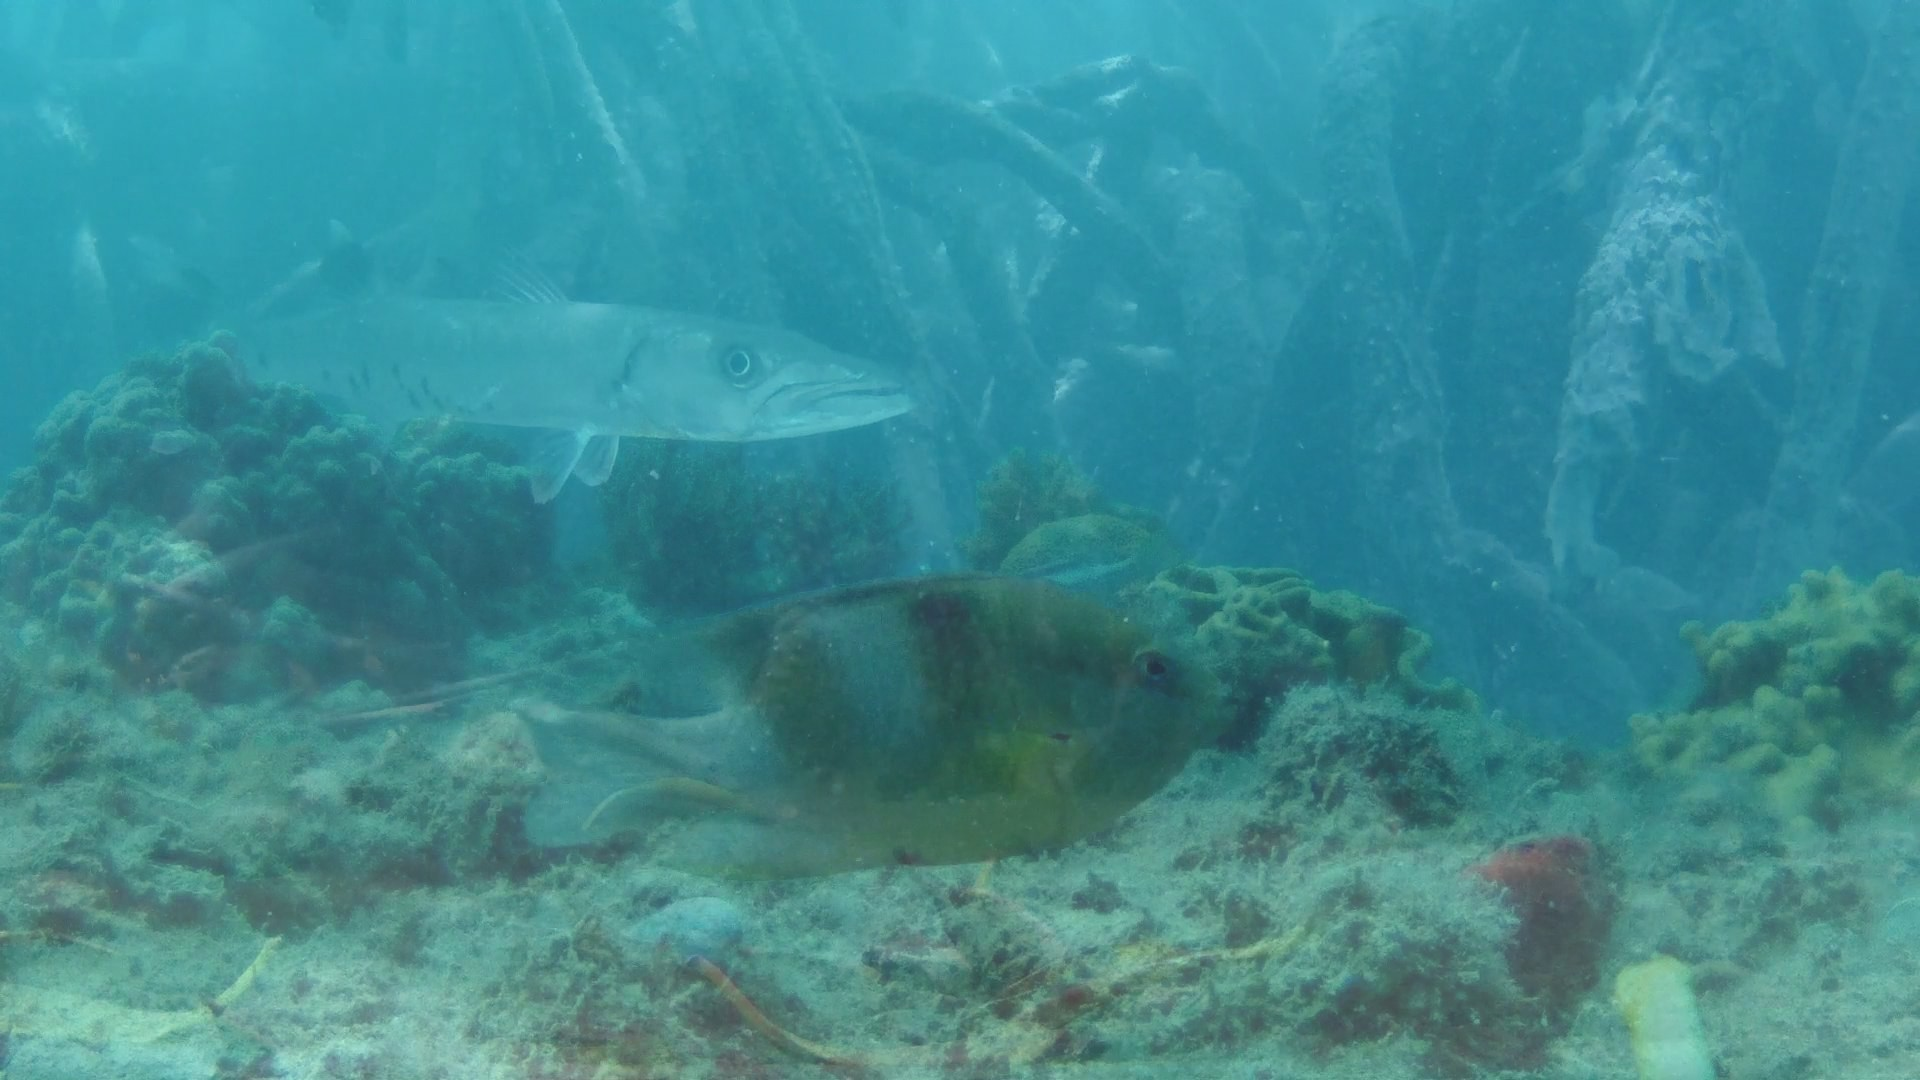
\includegraphics[width=0.8\textwidth]{images/mixup_2.jpg}
\end{column}
\end{columns}

\vspace{0.3cm}

\begin{columns}
\begin{column}{0.5\textwidth}
	\centering
	\textbf{Mosaic feature}
	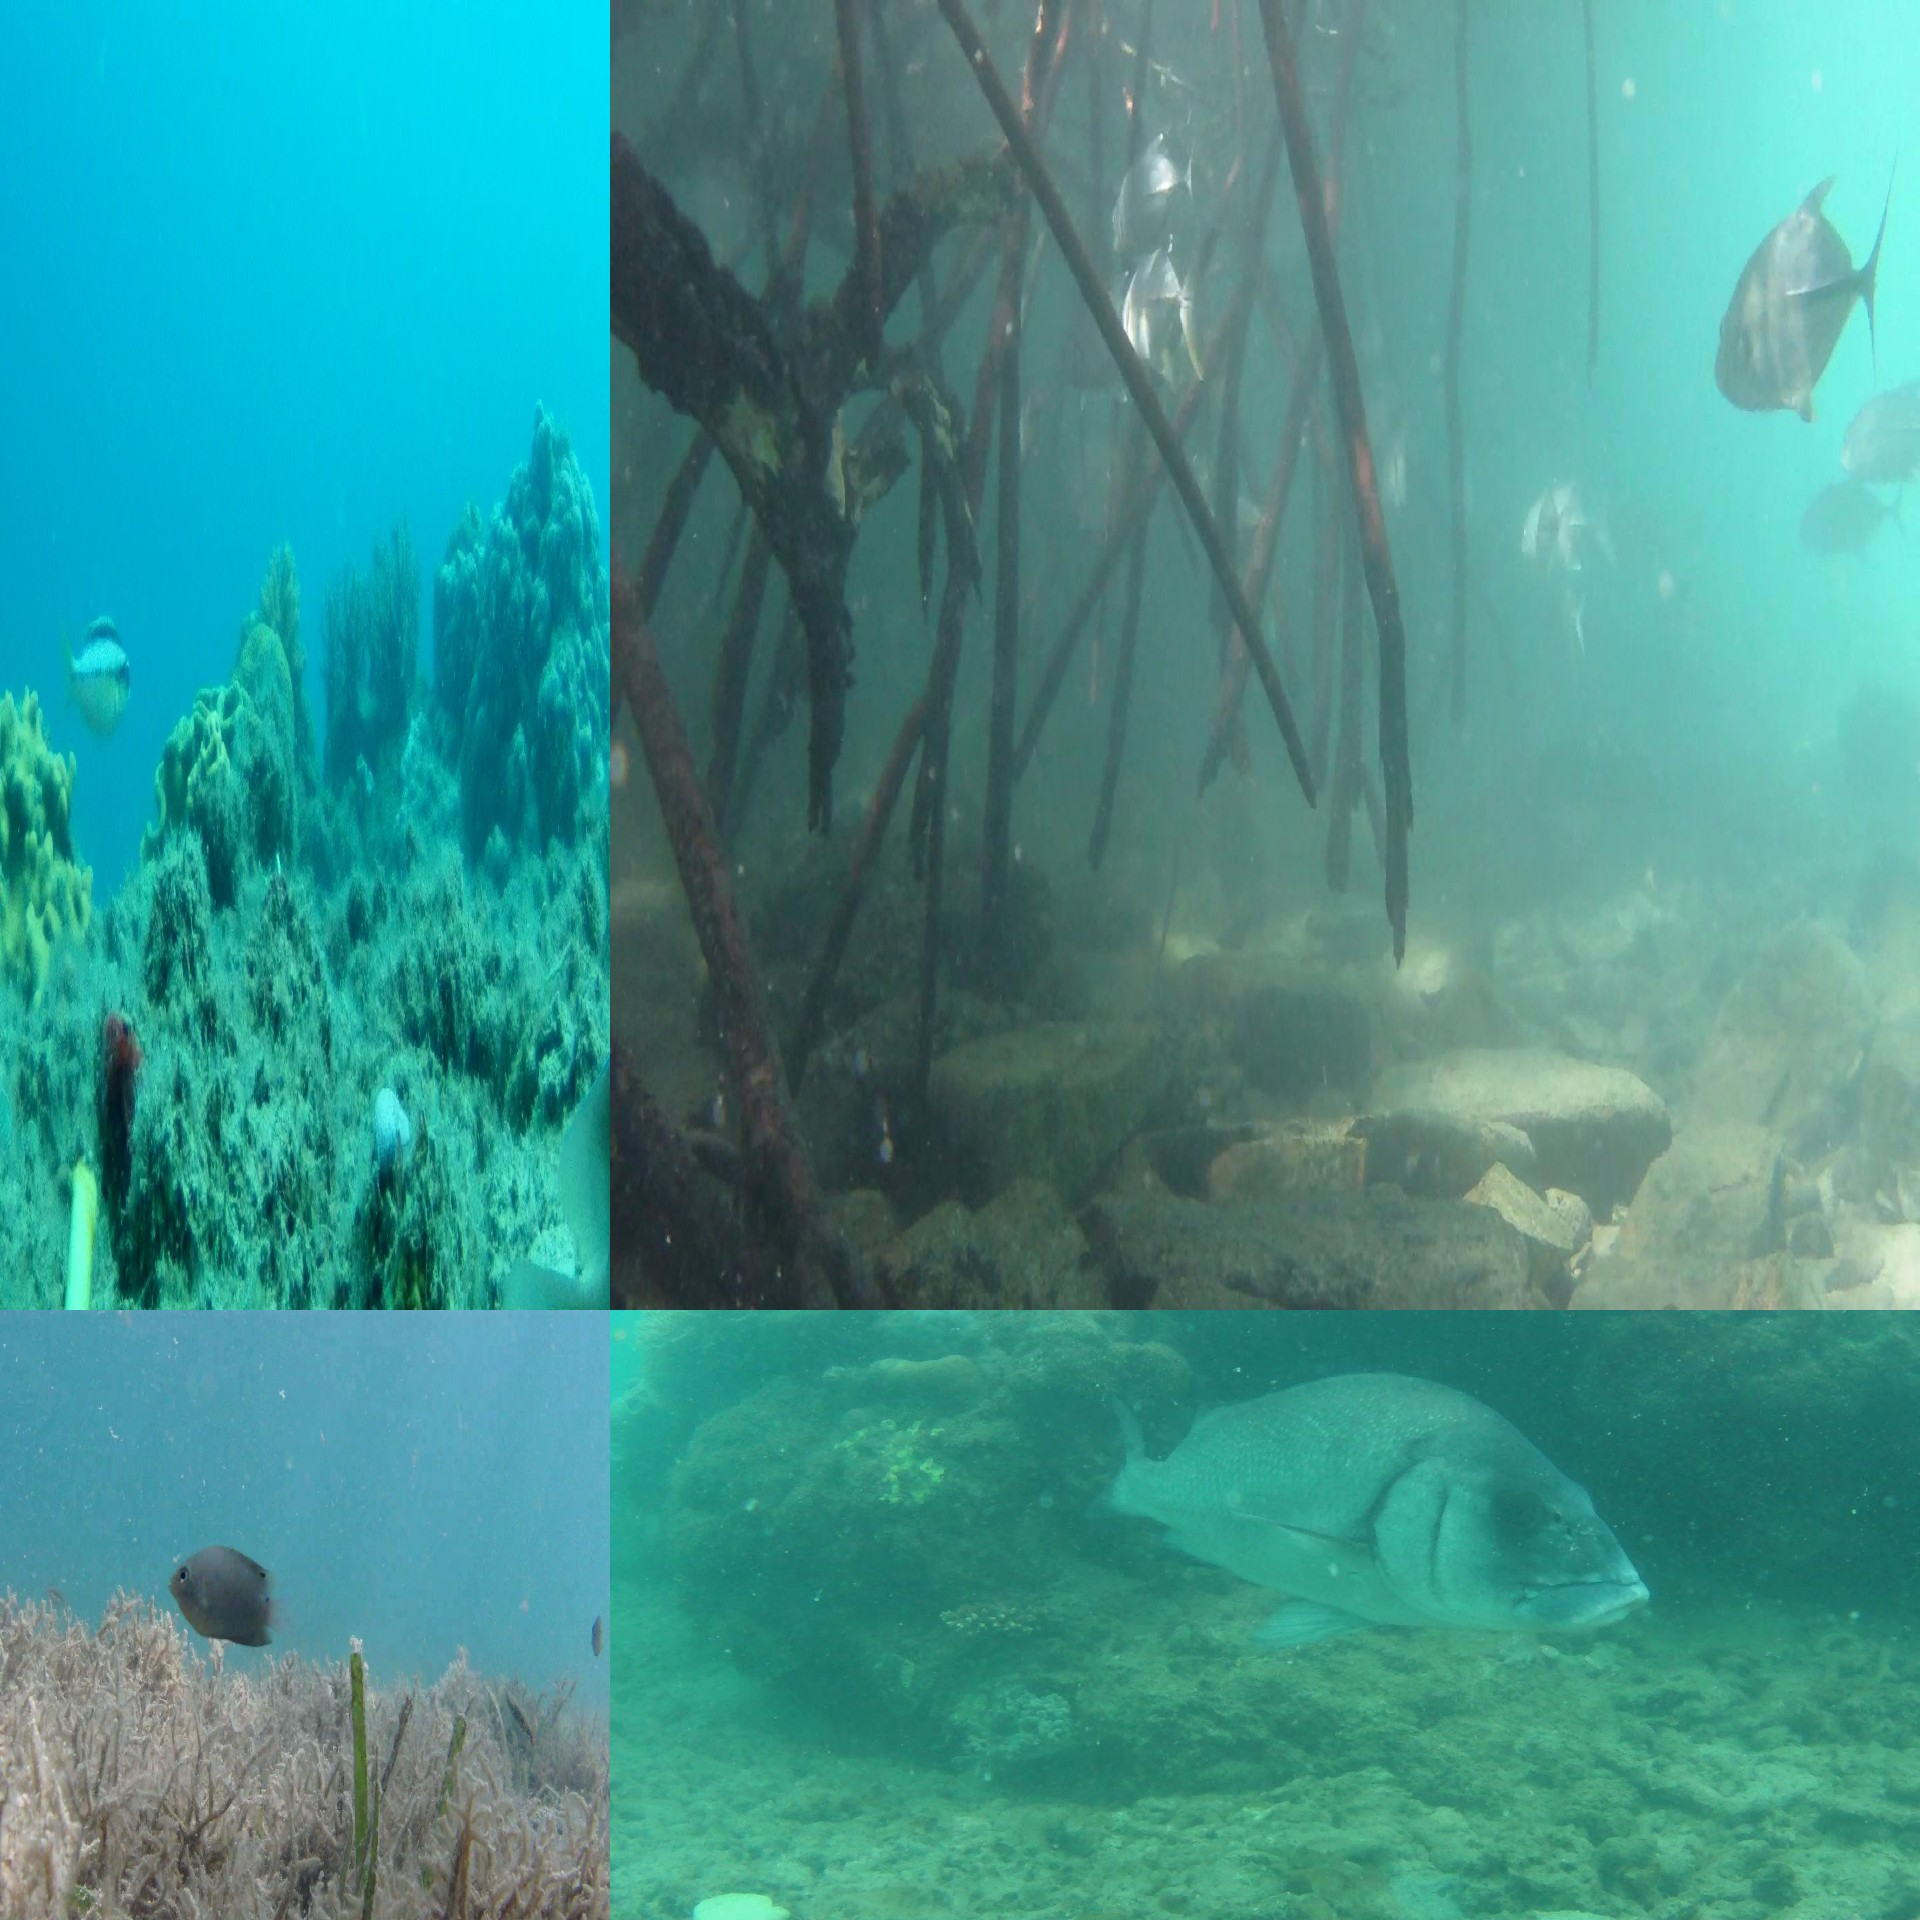
\includegraphics[width=0.8\textwidth]{images/mosaic.jpg}	
\end{column}

\begin{column}{0.5\textwidth}
	\centering
	\textbf{Cutout feature}
	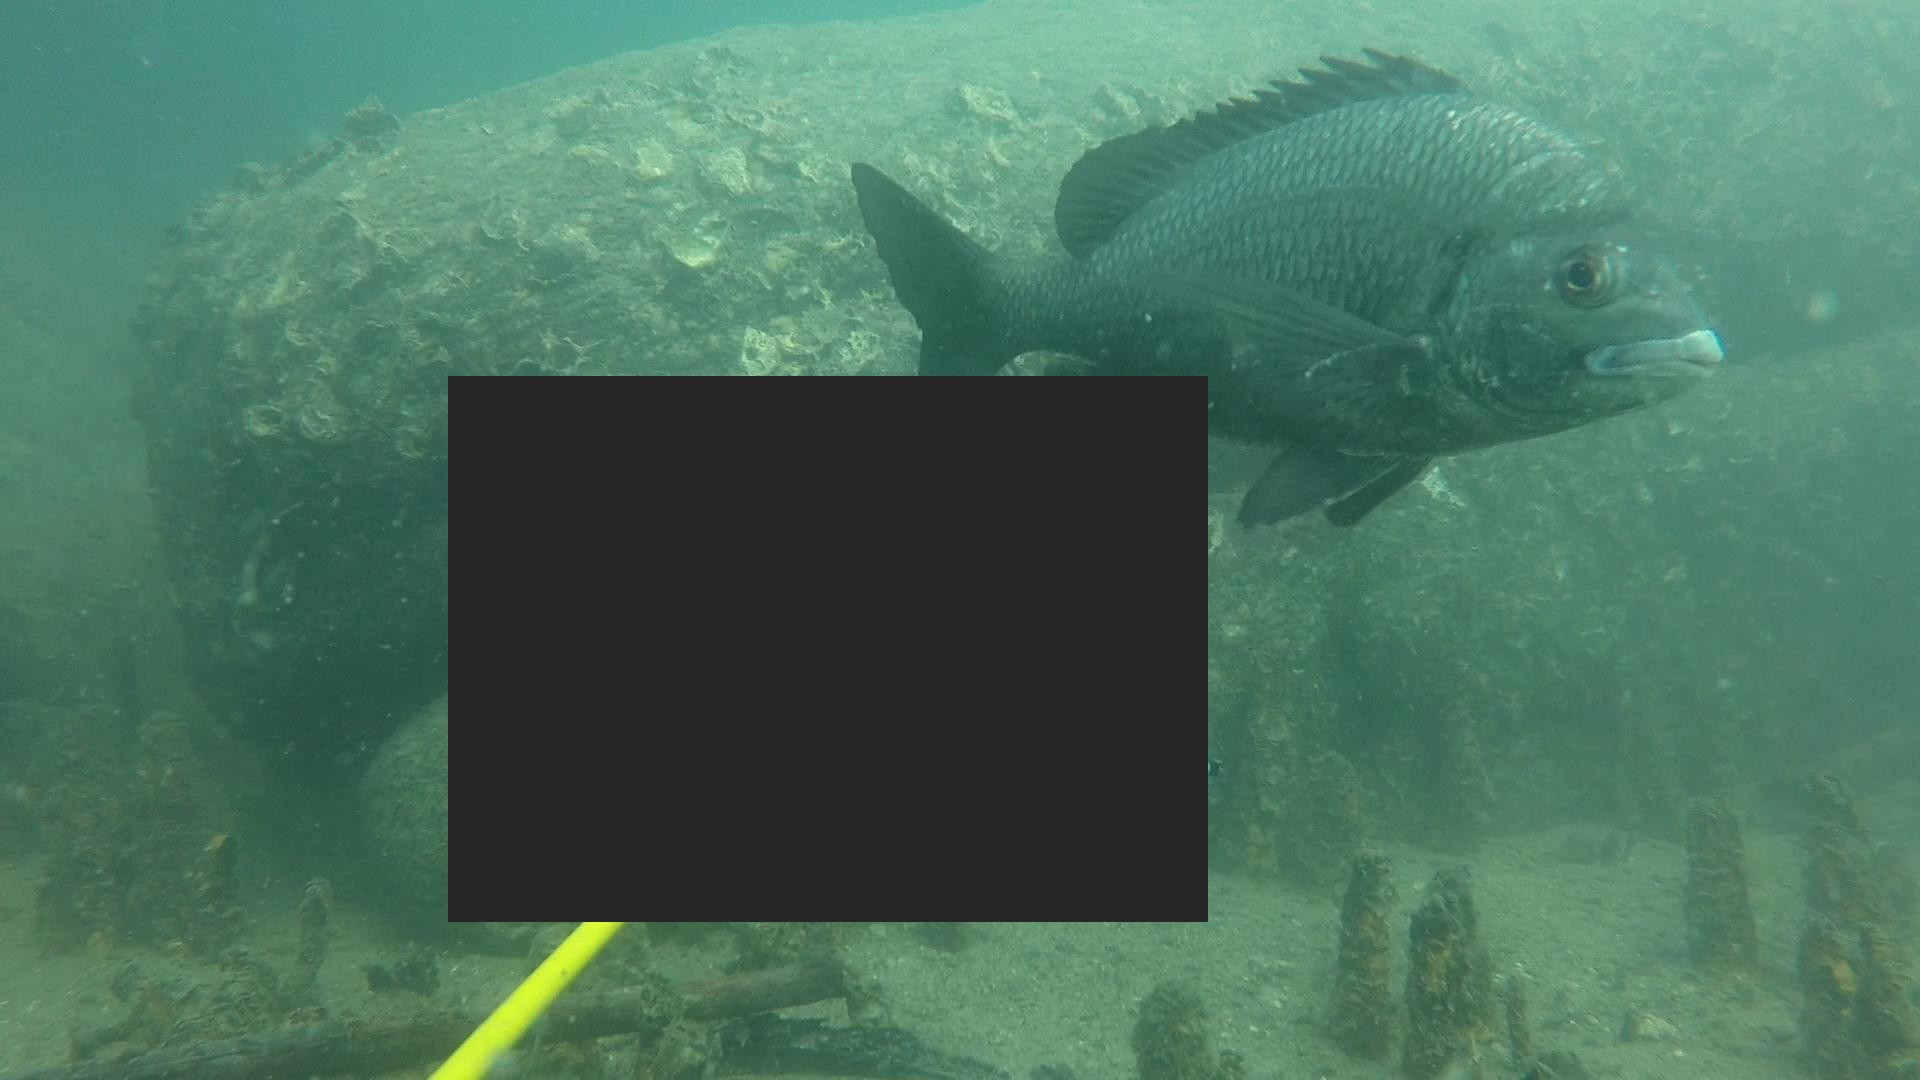
\includegraphics[width=0.8\textwidth]{images/cutout.jpg}
\end{column}
\end{columns}

\end{frame}

\begin{frame}
\frametitle{NMS}
The \textbf{Non-Maximum Suppression} is a technique that cleans up the output of a detection model by filtering out redundant and overlapping bounding boxes (high IoU) to ensure that each object is identified only once. 
\begin{enumerate}
	\item Sort by confidence score
	\item Remove high-IoU boxes 
	\item Repeat
\end{enumerate}
(IoU means Intersection over Union and the higher it is for a box, the more it overlaps the others)
\end{frame}

\begin{frame}
\frametitle{Inference}
\centering
\begin{columns}
\begin{column}{0.5\textwidth}
	\centering
	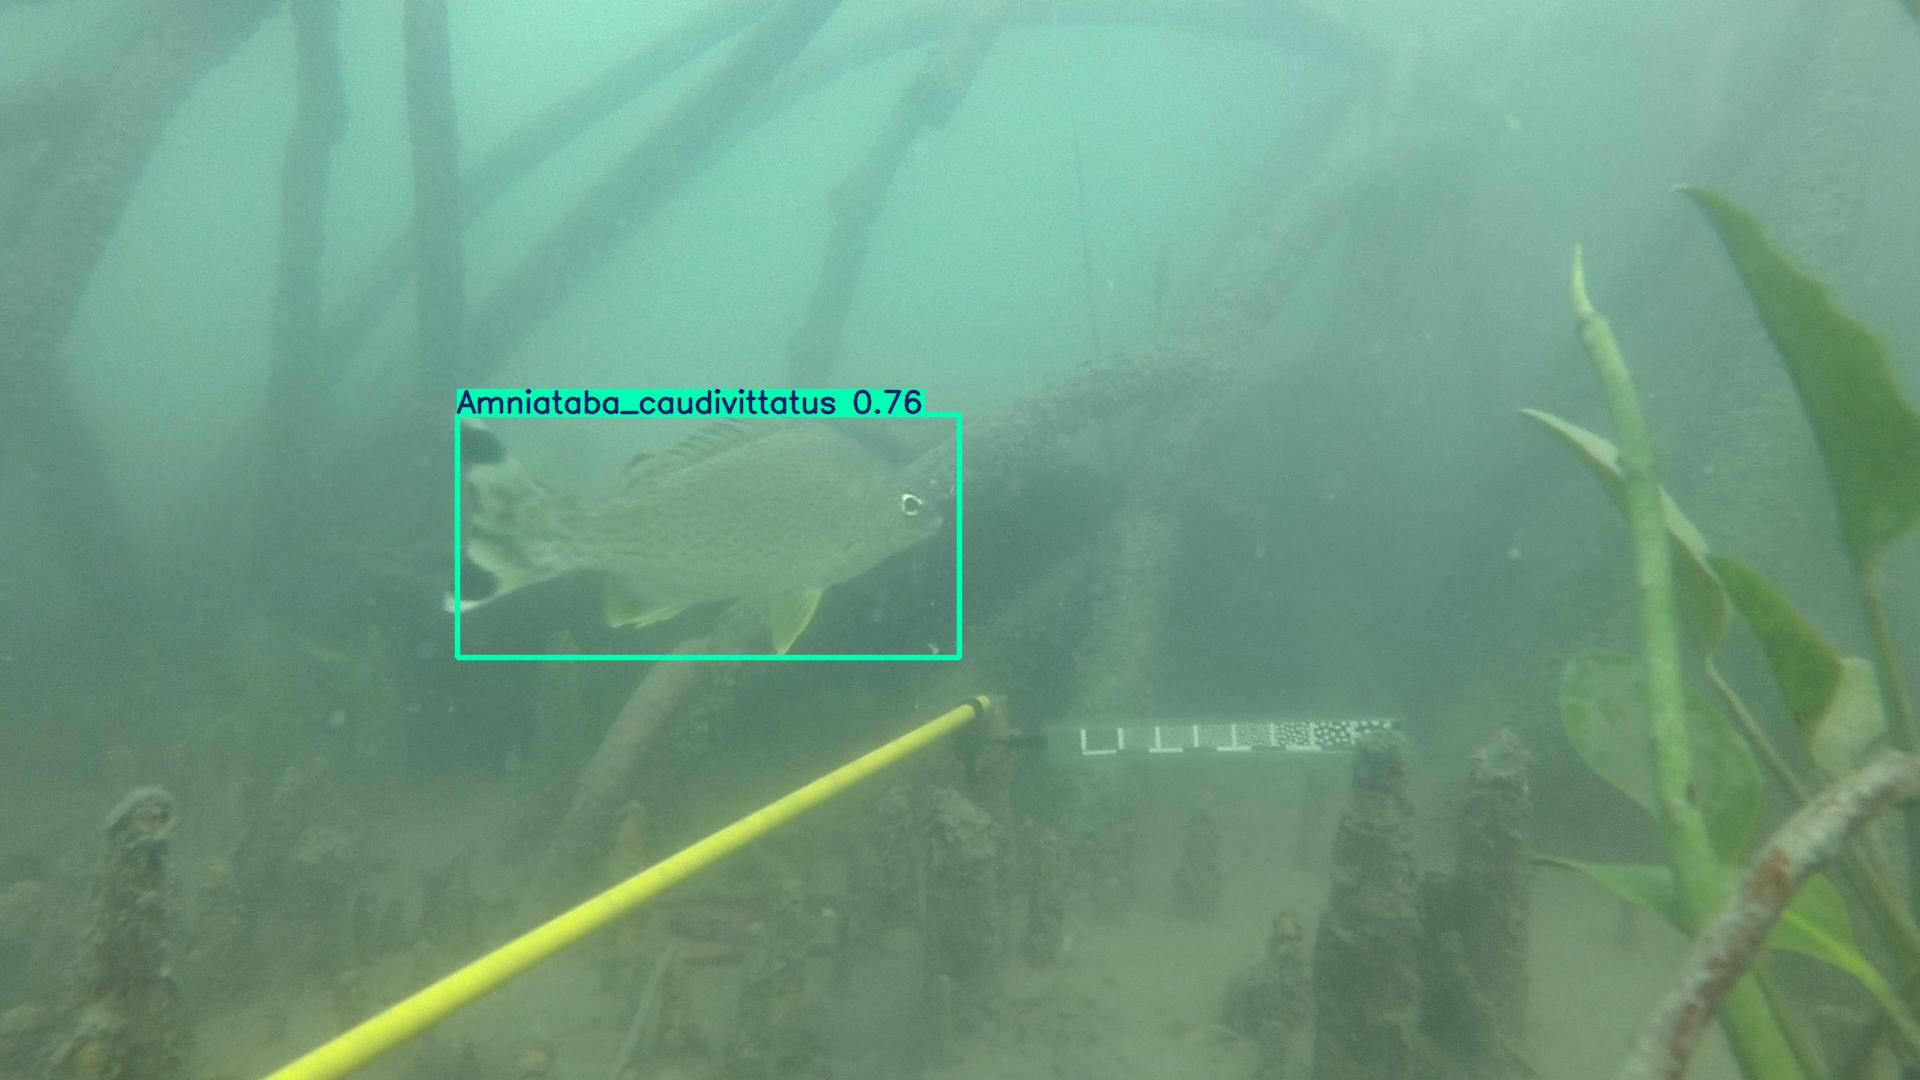
\includegraphics[width=\textwidth]{images/9894_Amniataba_caudivittatus_f000002.jpg}
\end{column}

\begin{column}{0.5\textwidth}
	\centering
	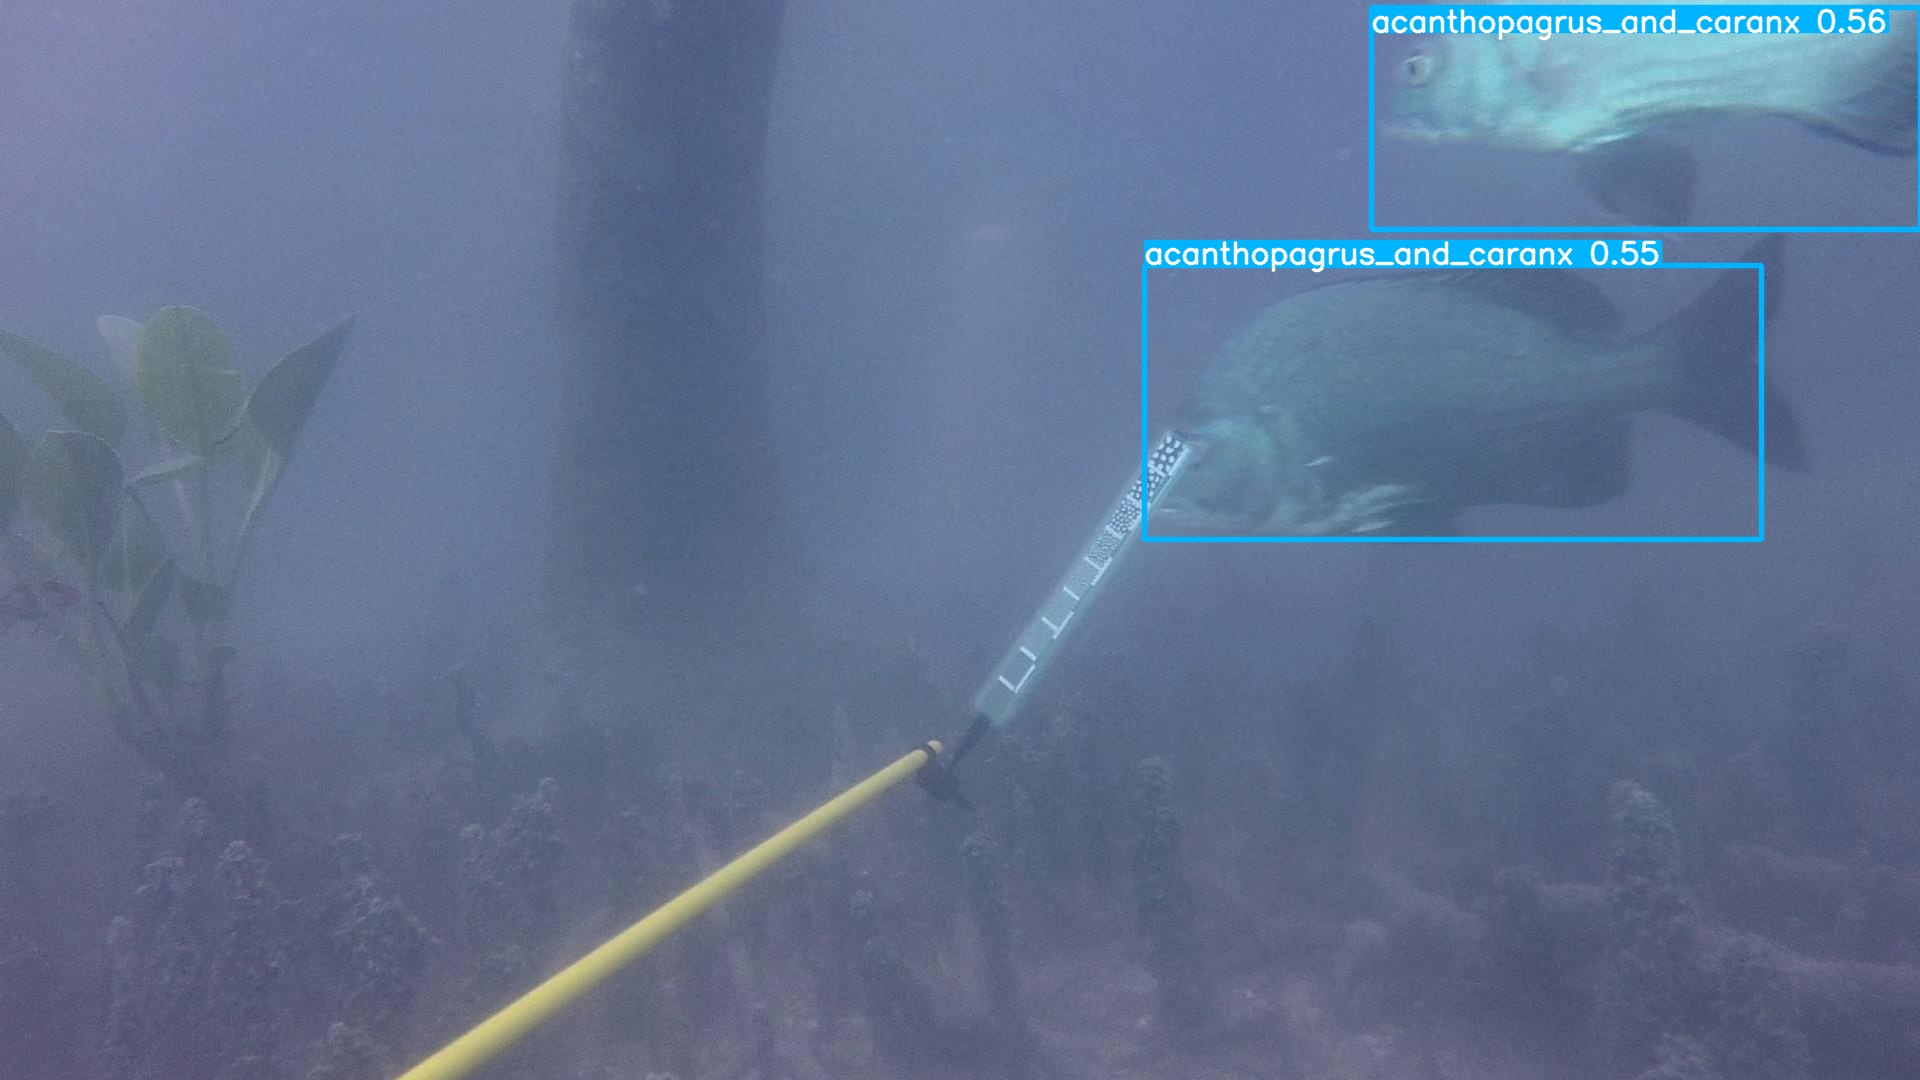
\includegraphics[width=\textwidth]{images/9866_acanthopagrus_and_caranx_f000041.jpg}
\end{column}
\end{columns}

\begin{columns}
\begin{column}{0.5\textwidth}
	\centering
	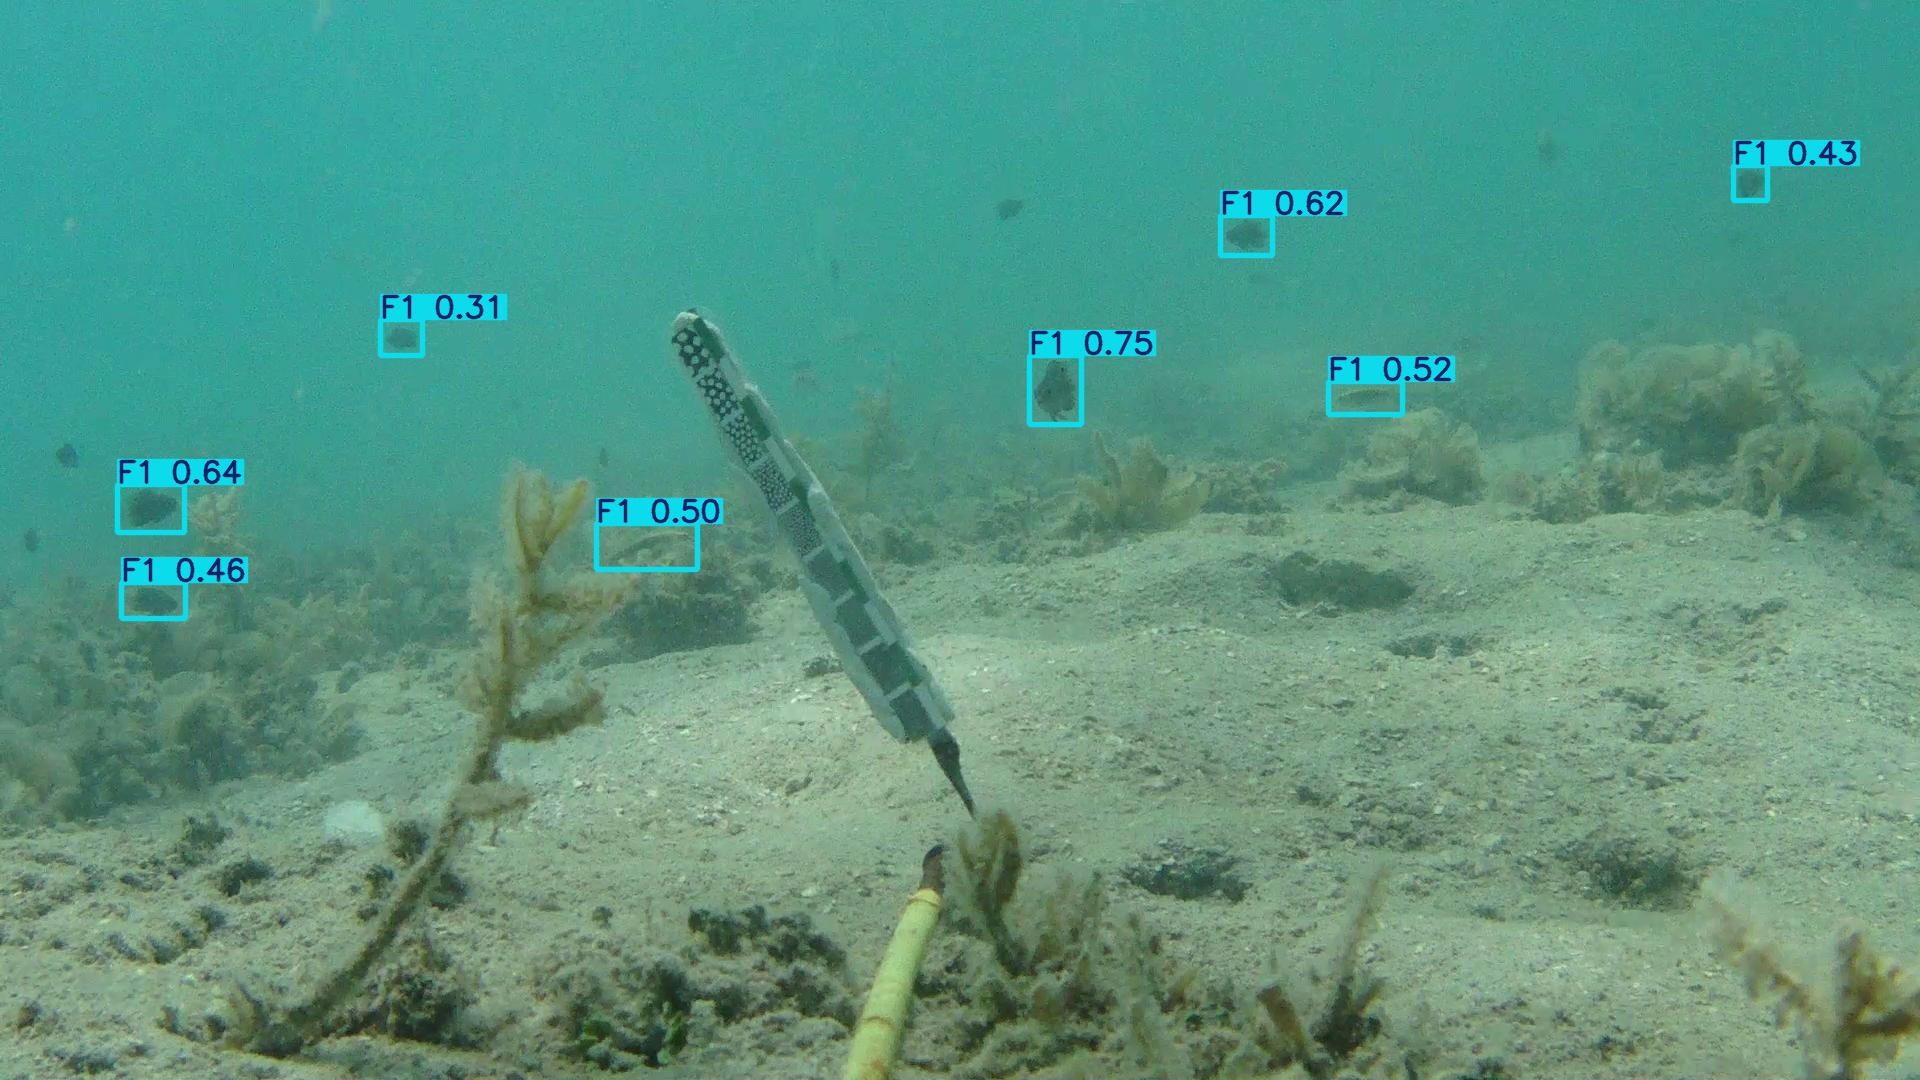
\includegraphics[width=\textwidth]{images/7268_F1_f000242.jpg}	
\end{column}

\begin{column}{0.5\textwidth}
	\centering
	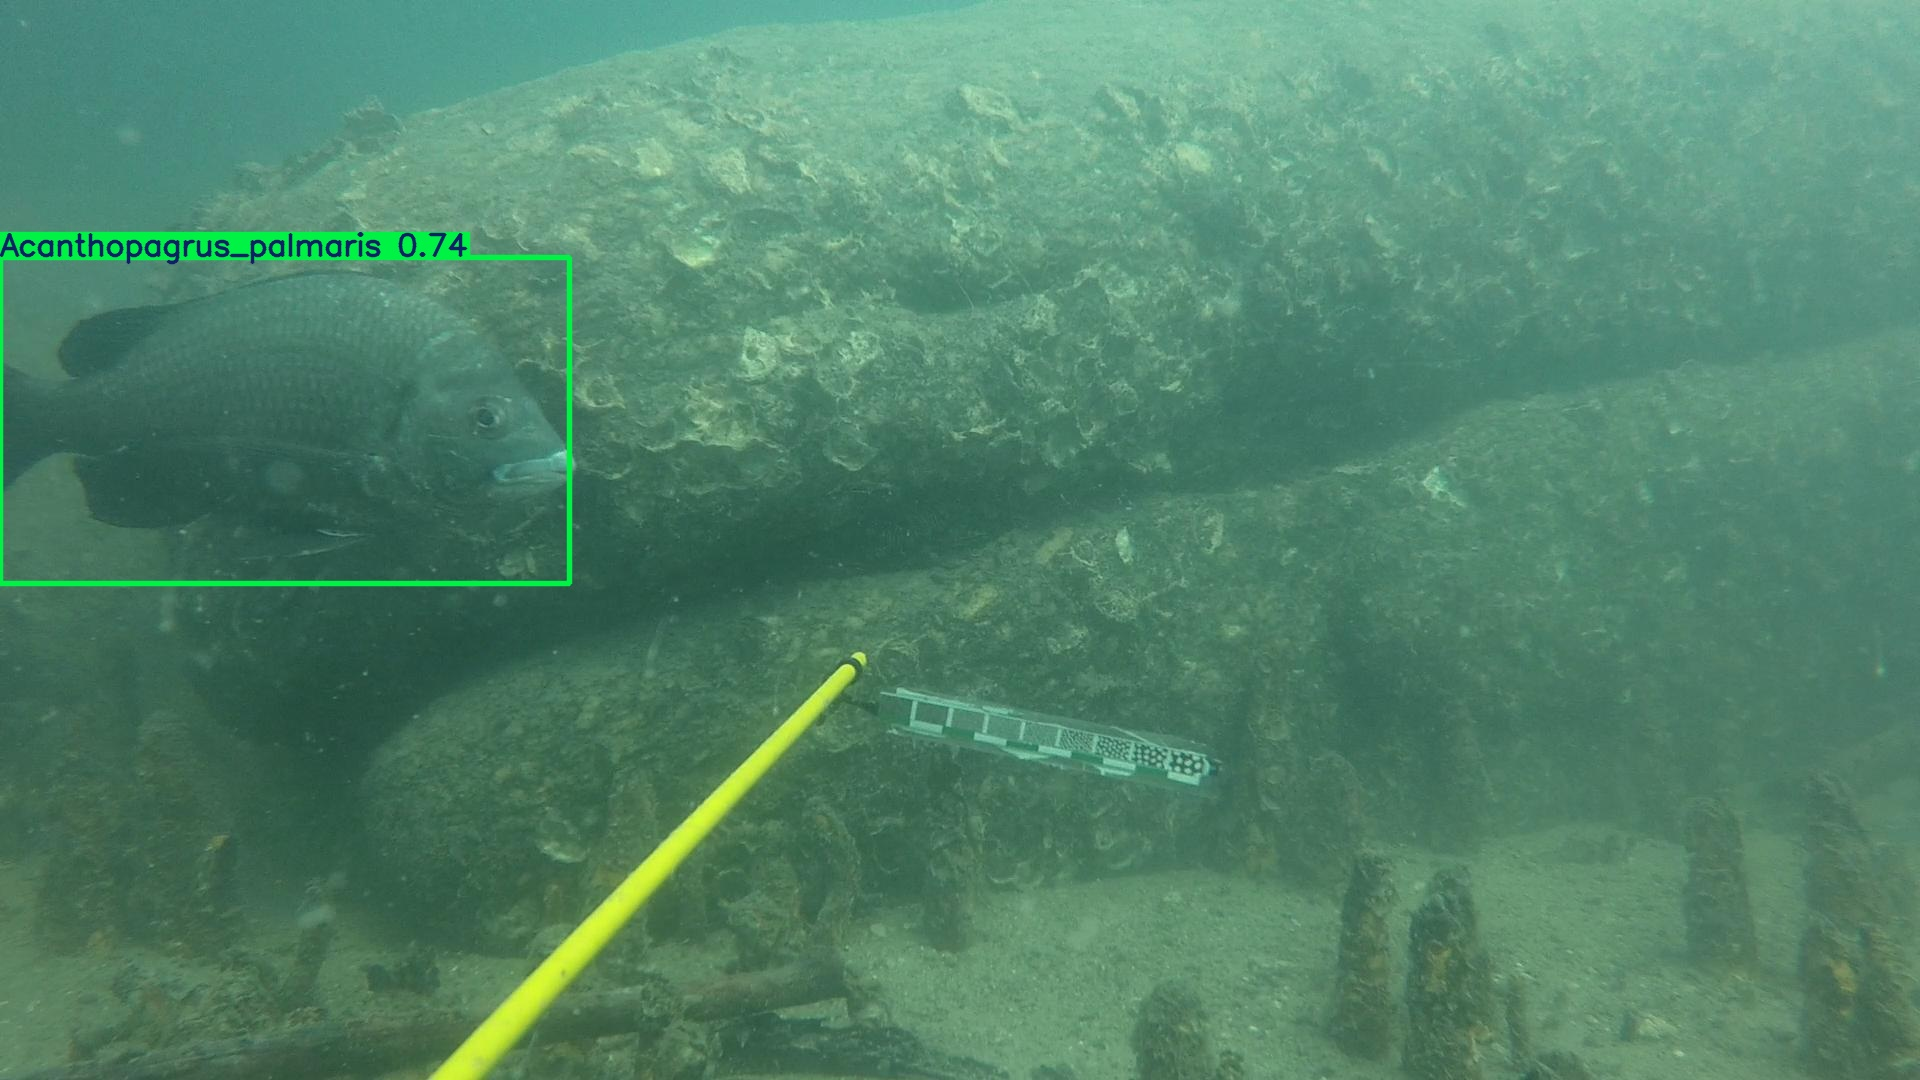
\includegraphics[width=\textwidth]{images/9908_Acanthopagrus_palmaris_f000010.jpg}
\end{column}
\end{columns}


\end{frame}

\section{Tracking}

\begin{frame}
    \frametitle{The Tracking Challenge: Occlusion \& ID Switches}
    
    \begin{columns}[T,totalwidth=\textwidth] 
        \begin{column}{0.32\textwidth}
            \centering
            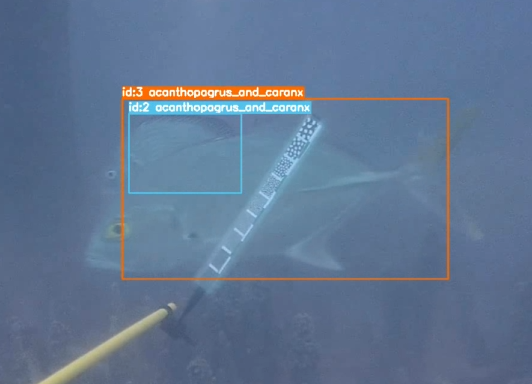
\includegraphics[width=\linewidth]{images/wrong_occlusion_1.png}
            \vspace{0.5em}
            \tiny
            \textbf{1. Before Occlusion} \\
            The fish ID 2 is clearly visible and being tracked.
        \end{column}
        
        \begin{column}{0.32\textwidth}
            \centering
            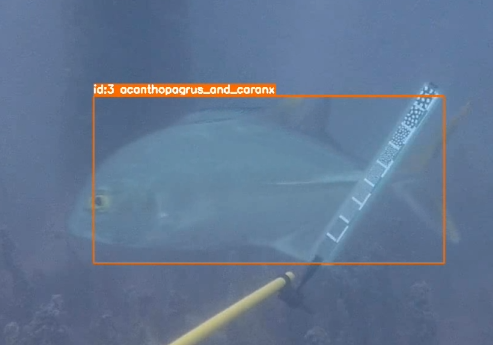
\includegraphics[width=\linewidth]{images/wrong_occlusion_2.png}
            \vspace{0.5em}
            \tiny
            \textbf{2. During Occlusion} \\
            Fish ID 2 is now hidden behind fish ID 3.
        \end{column}
        
        \begin{column}{0.32\textwidth}
            \centering
            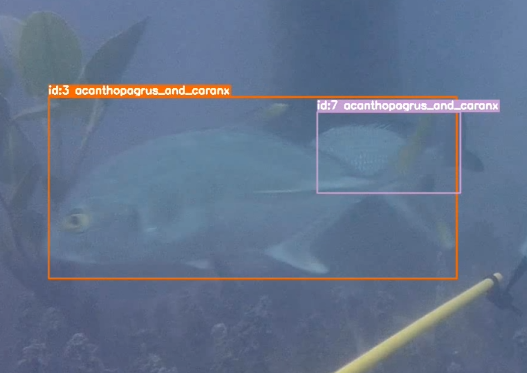
\includegraphics[width=\linewidth]{images/wrong_occlusion_3.png}
            \vspace{0.5em}
            \tiny
            \textbf{3. After Occlusion (ID Switch)} \\
            The fish reappears identified as a new object ID 7.
        \end{column}
    \end{columns}
\end{frame}


\begin{frame}
    \frametitle{The ByteTrack Algorithm}
    
    \begin{figure}
        \centering
        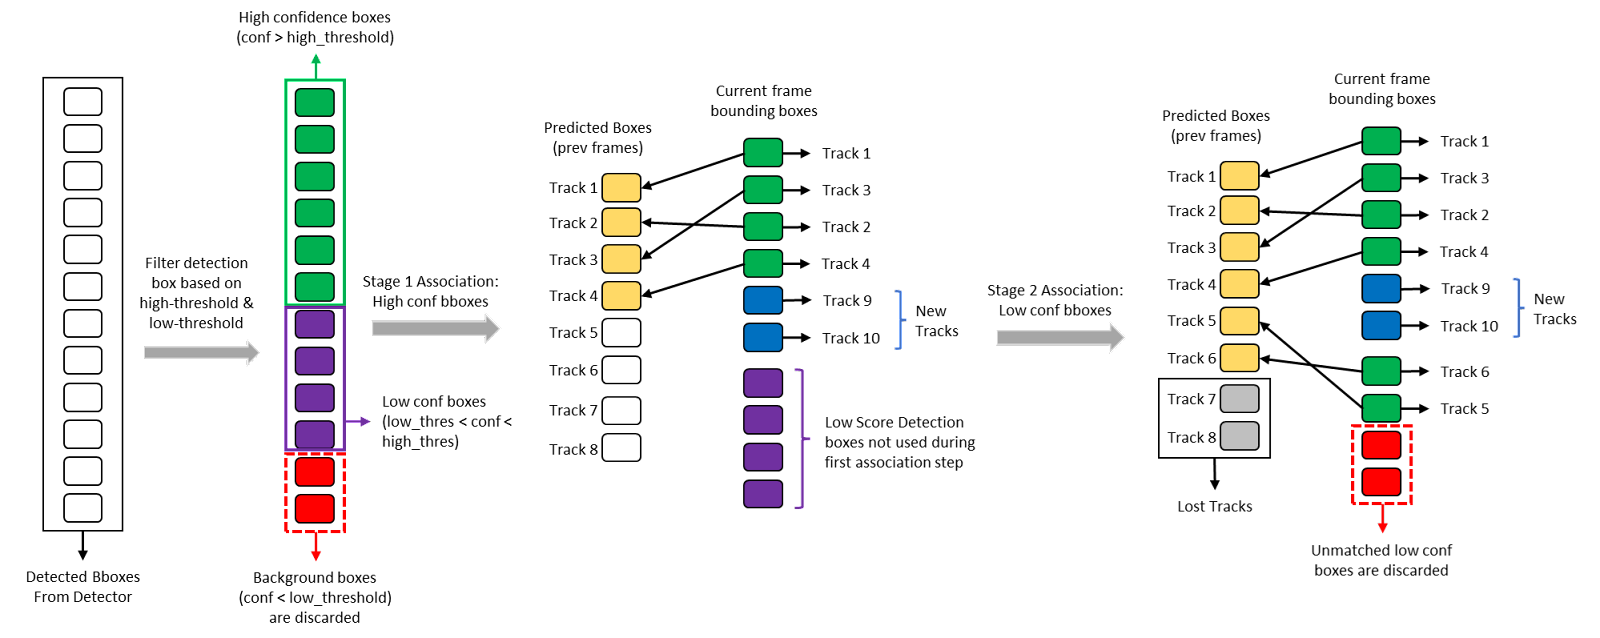
\includegraphics[width=1\linewidth]{images/bytetrack.png}
        \footnote{\cite{datature2024bytetrack}}
    \end{figure}
    
\end{frame}

\begin{frame}
    \frametitle{Correct Object Re-identification}
    
    \begin{columns}[T,totalwidth=\textwidth] 
        \begin{column}{0.32\textwidth}
            \centering
            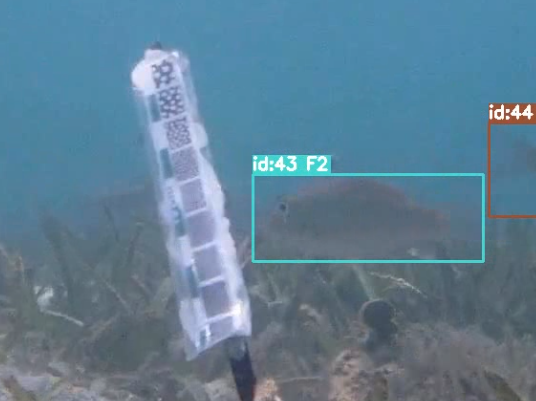
\includegraphics[width=\linewidth]{images/occlusion_1.png}
            \vspace{0.5em}
            \tiny
            \textbf{1. Before Occlusion} \\
            The fish ID 43 is clearly visible and being tracked.
        \end{column}
        
        \begin{column}{0.32\textwidth}
            \centering
            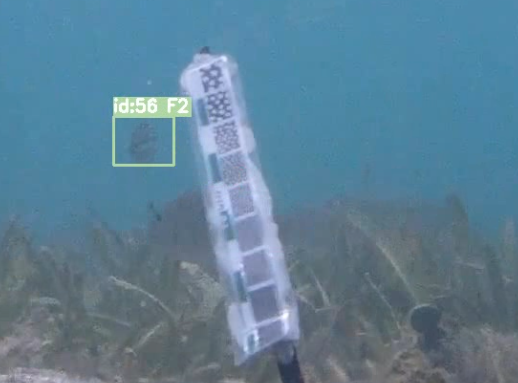
\includegraphics[width=\linewidth]{images/occlusion_2.png}
            \vspace{0.5em}
            \tiny
            \textbf{2. During Occlusion} \\
            Fish ID 43 is now hidden behind an object.
        \end{column}
        
        \begin{column}{0.32\textwidth}
            \centering
            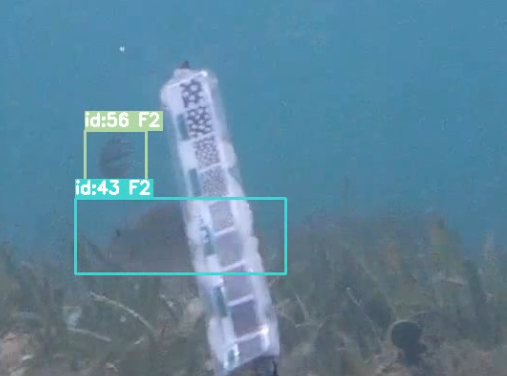
\includegraphics[width=\linewidth]{images/occlusion_3.png}
            \vspace{0.5em}
            \tiny
            \textbf{3. After Occlusion} \\
            The fish reappears. ByteTrack re-identifies it as ID 43.
        \end{column}
    \end{columns}
\end{frame}


\section{Results}

\begin{frame}{Fish Detection (DeepFish): Metrics}
    \centering

    \begin{minipage}{0.49\linewidth}
        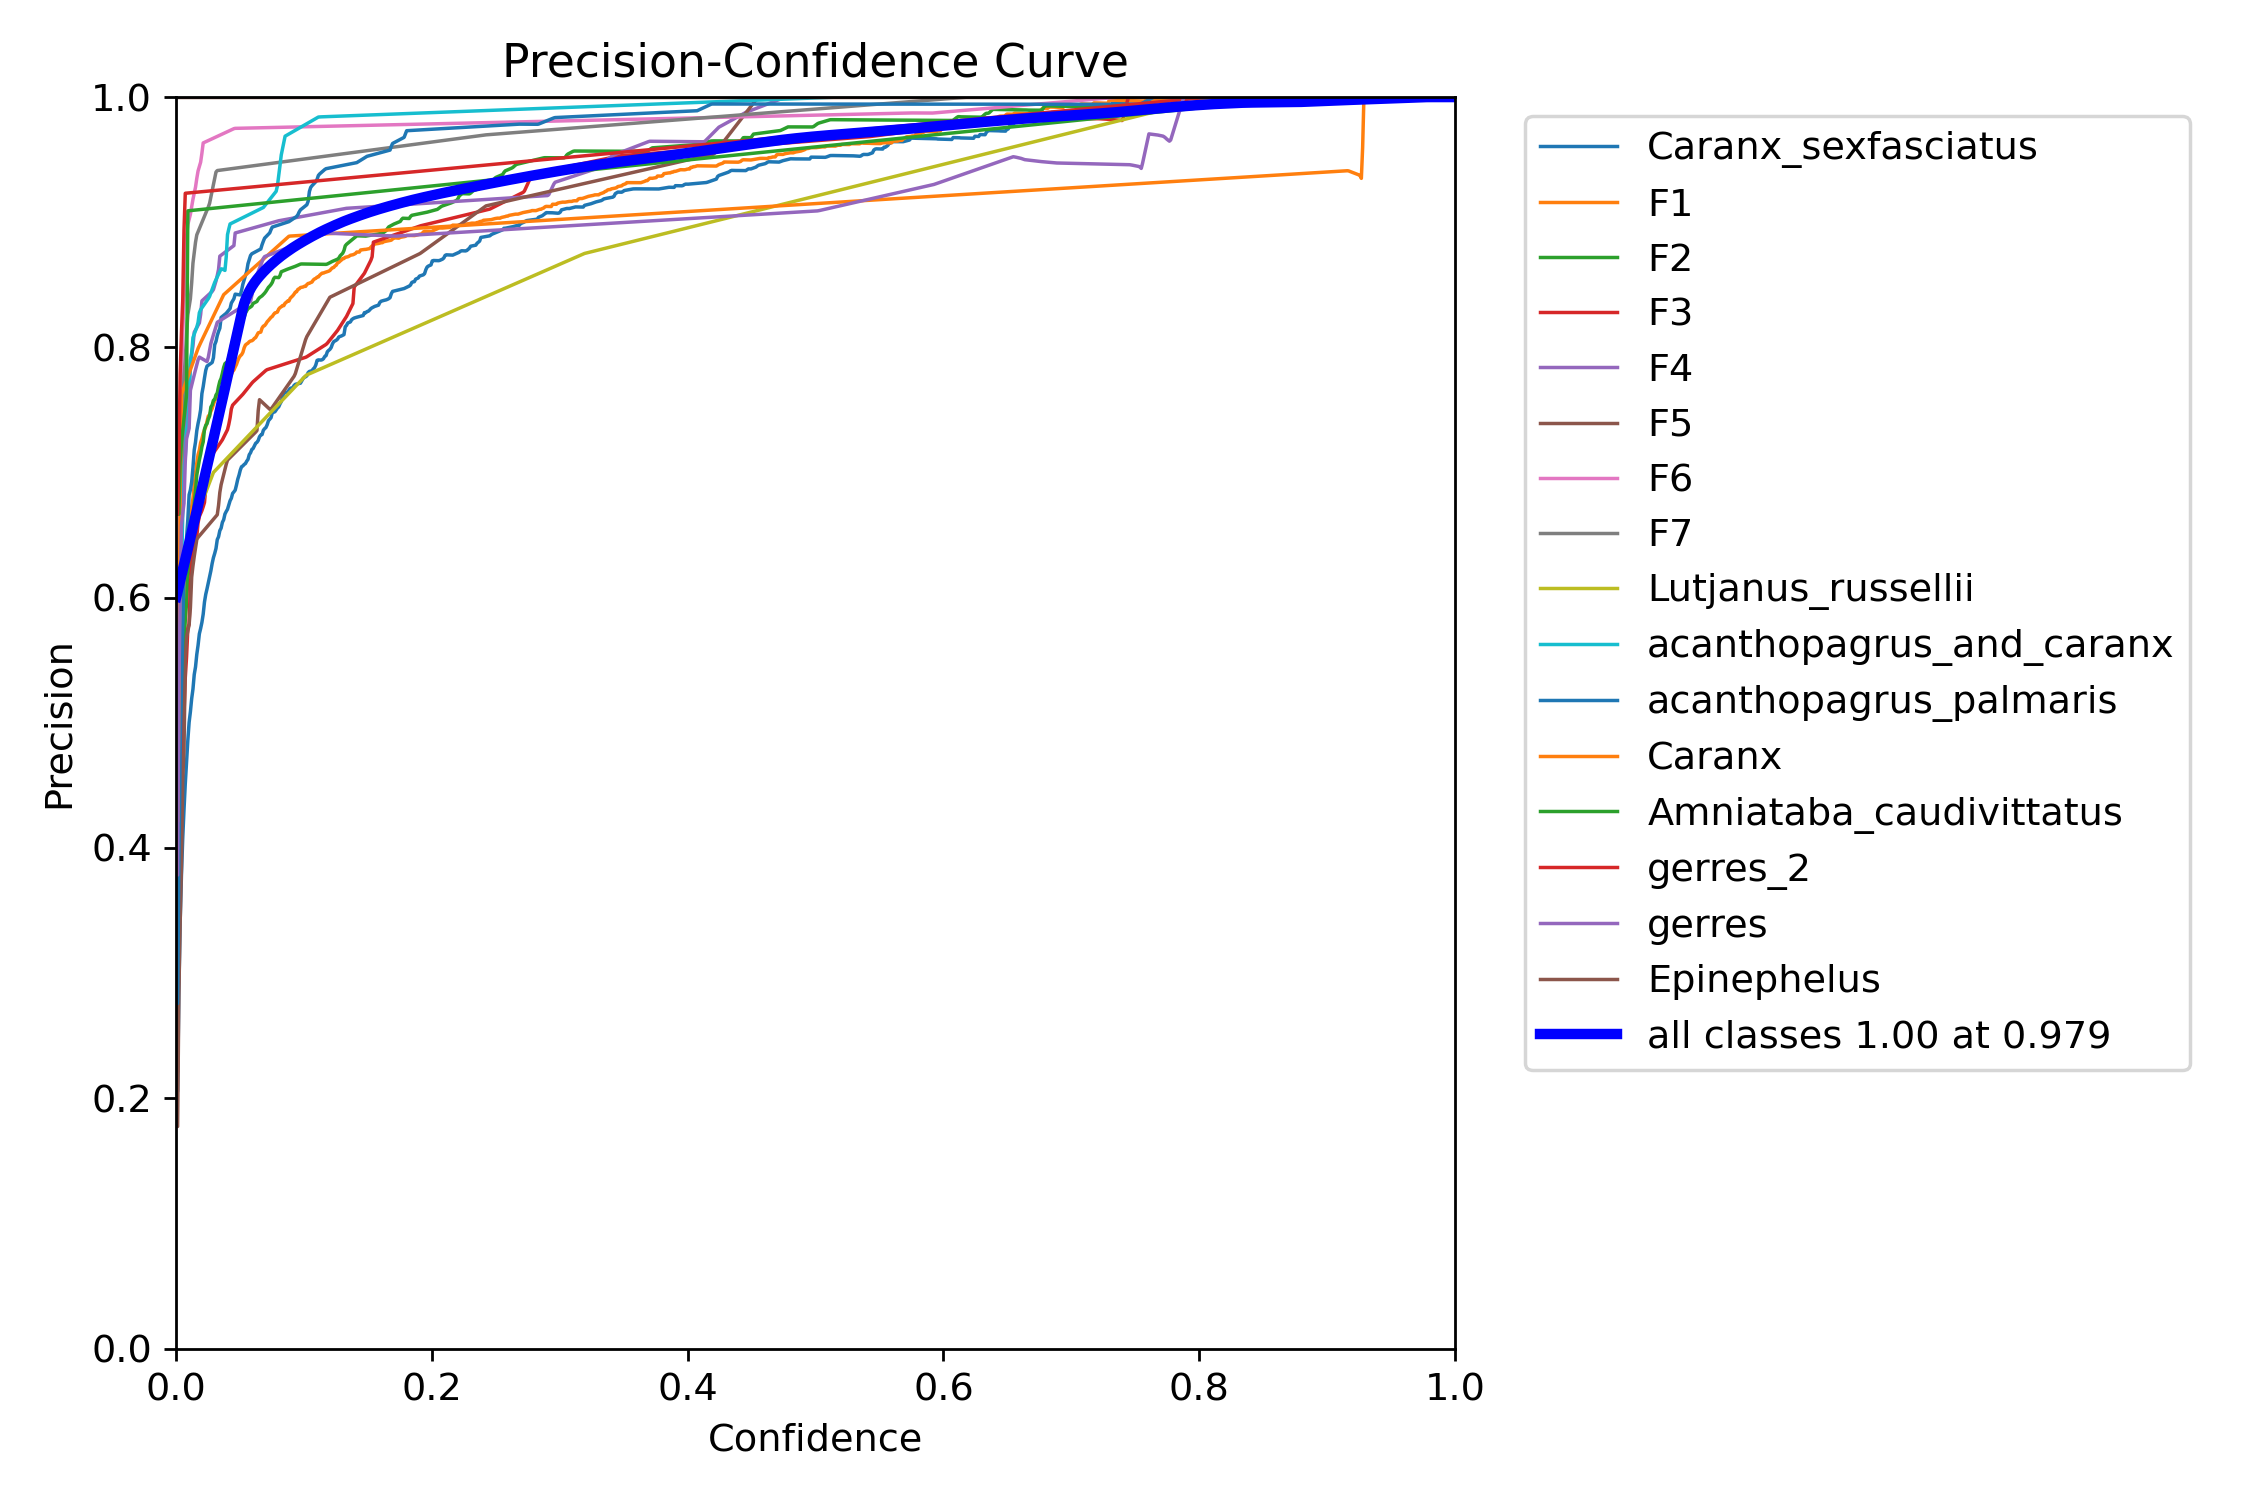
\includegraphics[width=\linewidth]{images/BoxP_curve.png}
    \end{minipage}
    \hfill
    \begin{minipage}{0.49\linewidth}
        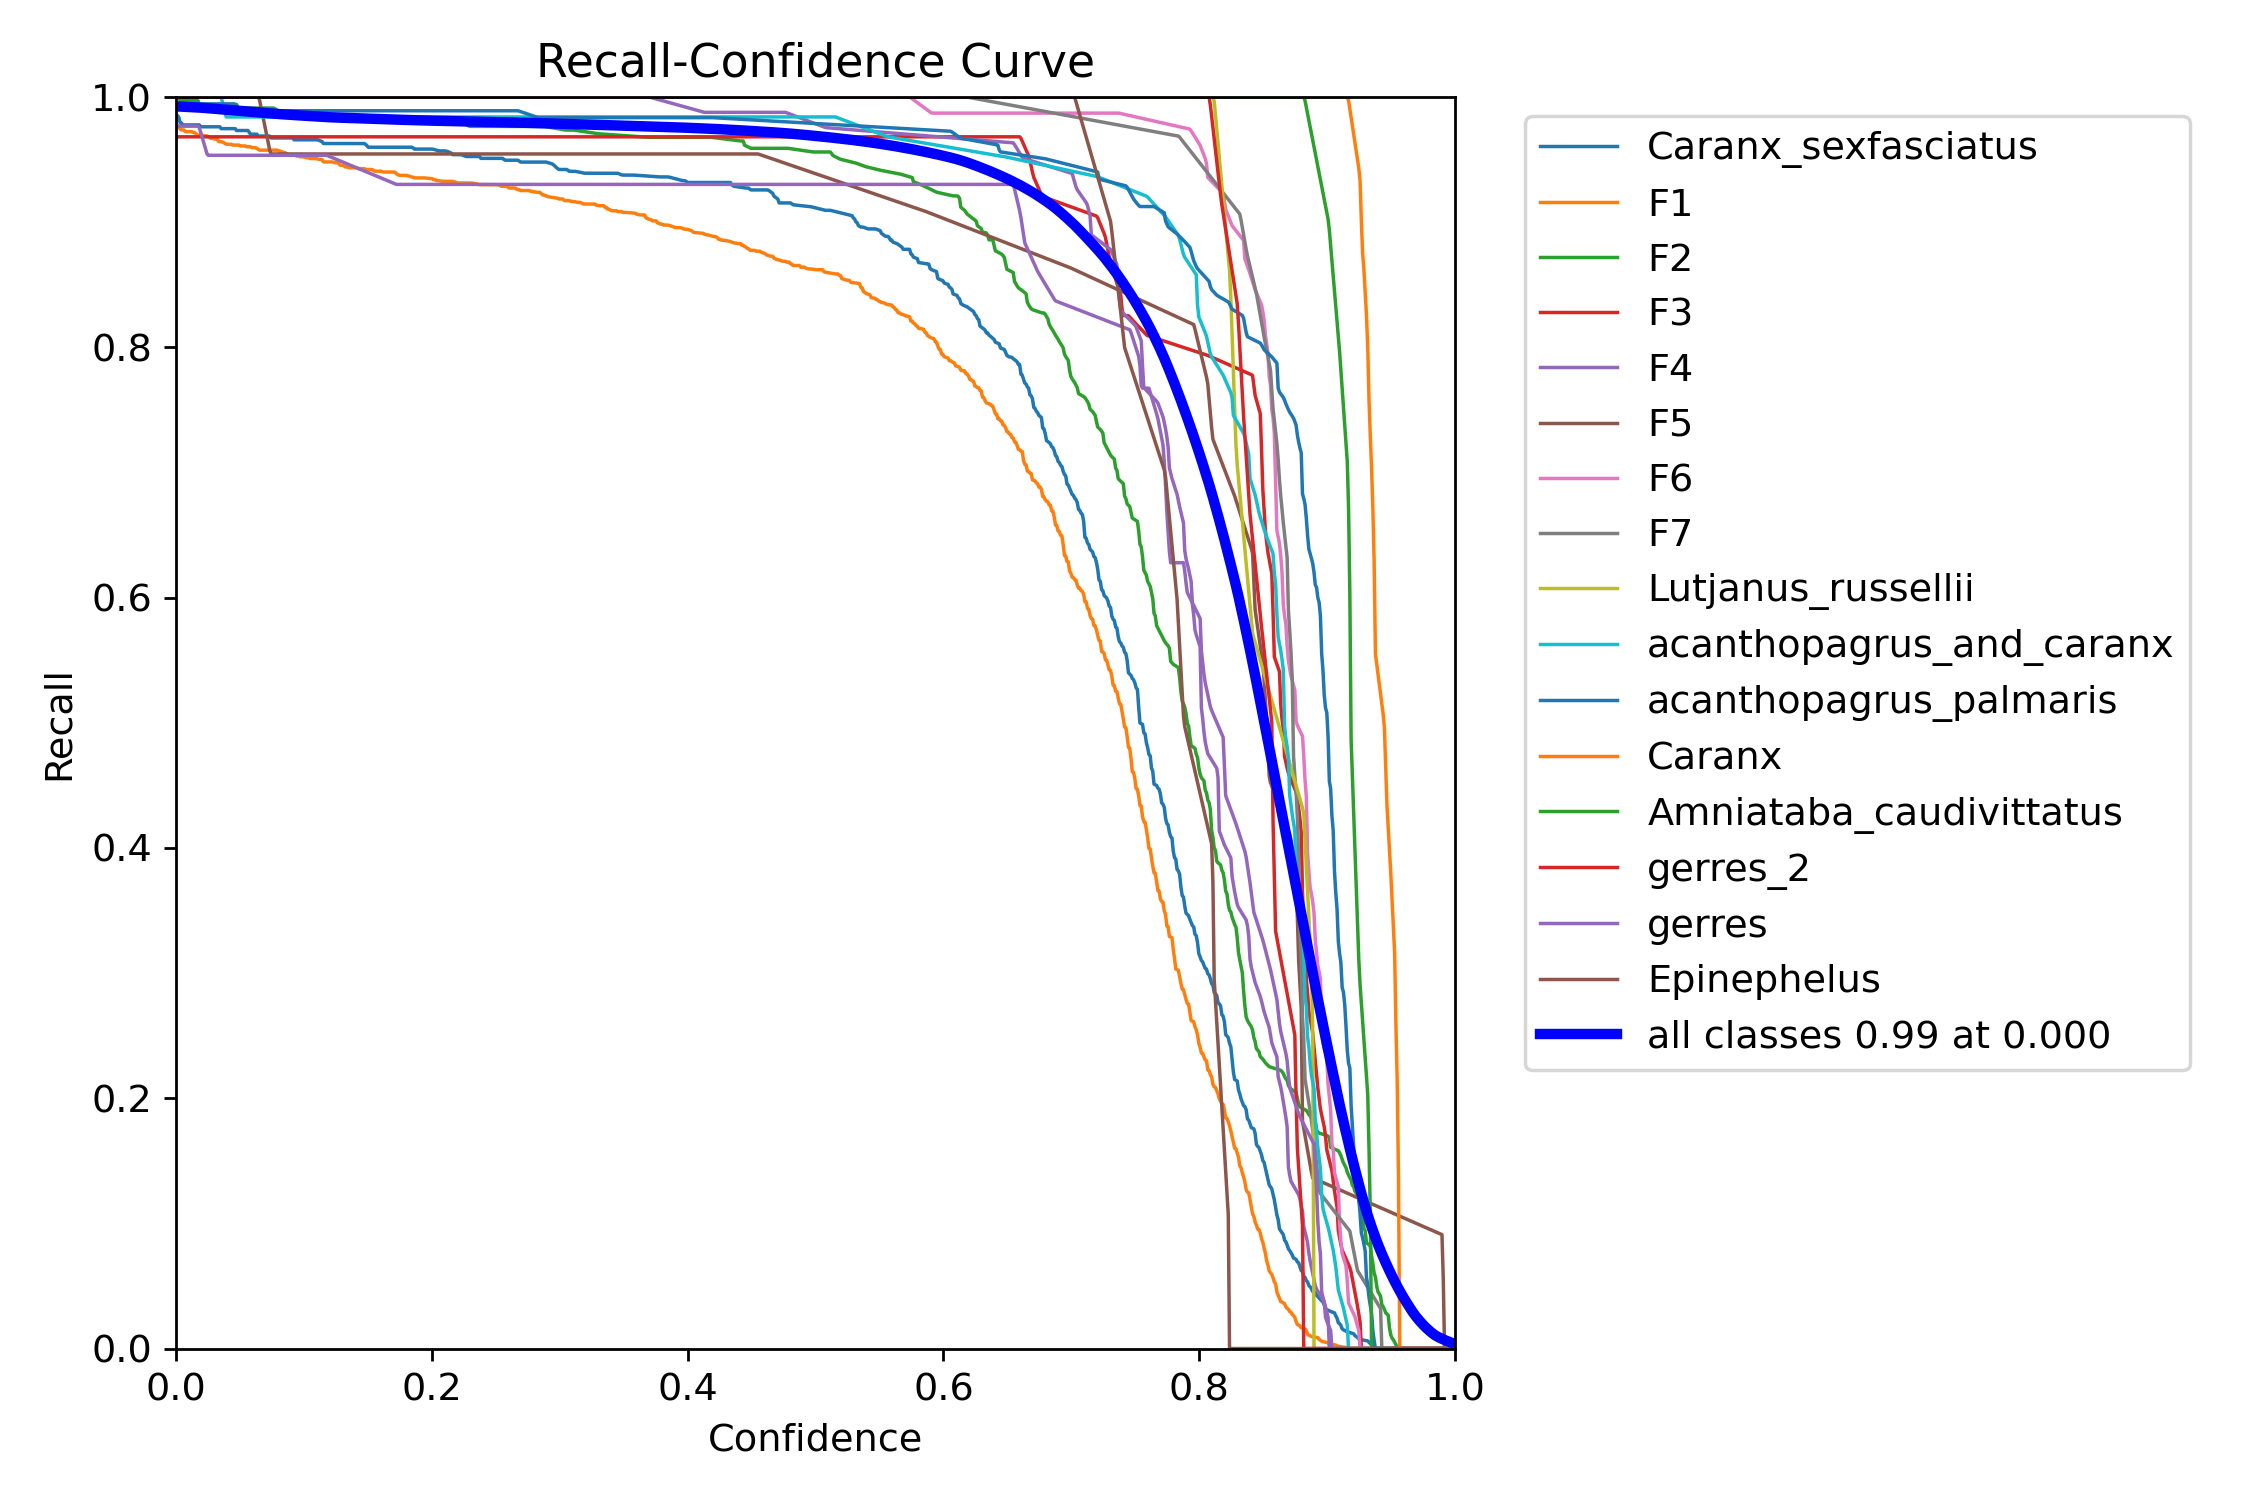
\includegraphics[width=\linewidth]{images/BoxR_curve.png}
    \end{minipage}
\end{frame}


\begin{frame}{Fish Detection (DeepFish): Metrics}
    \centering
    \begin{minipage}{0.49\linewidth}
        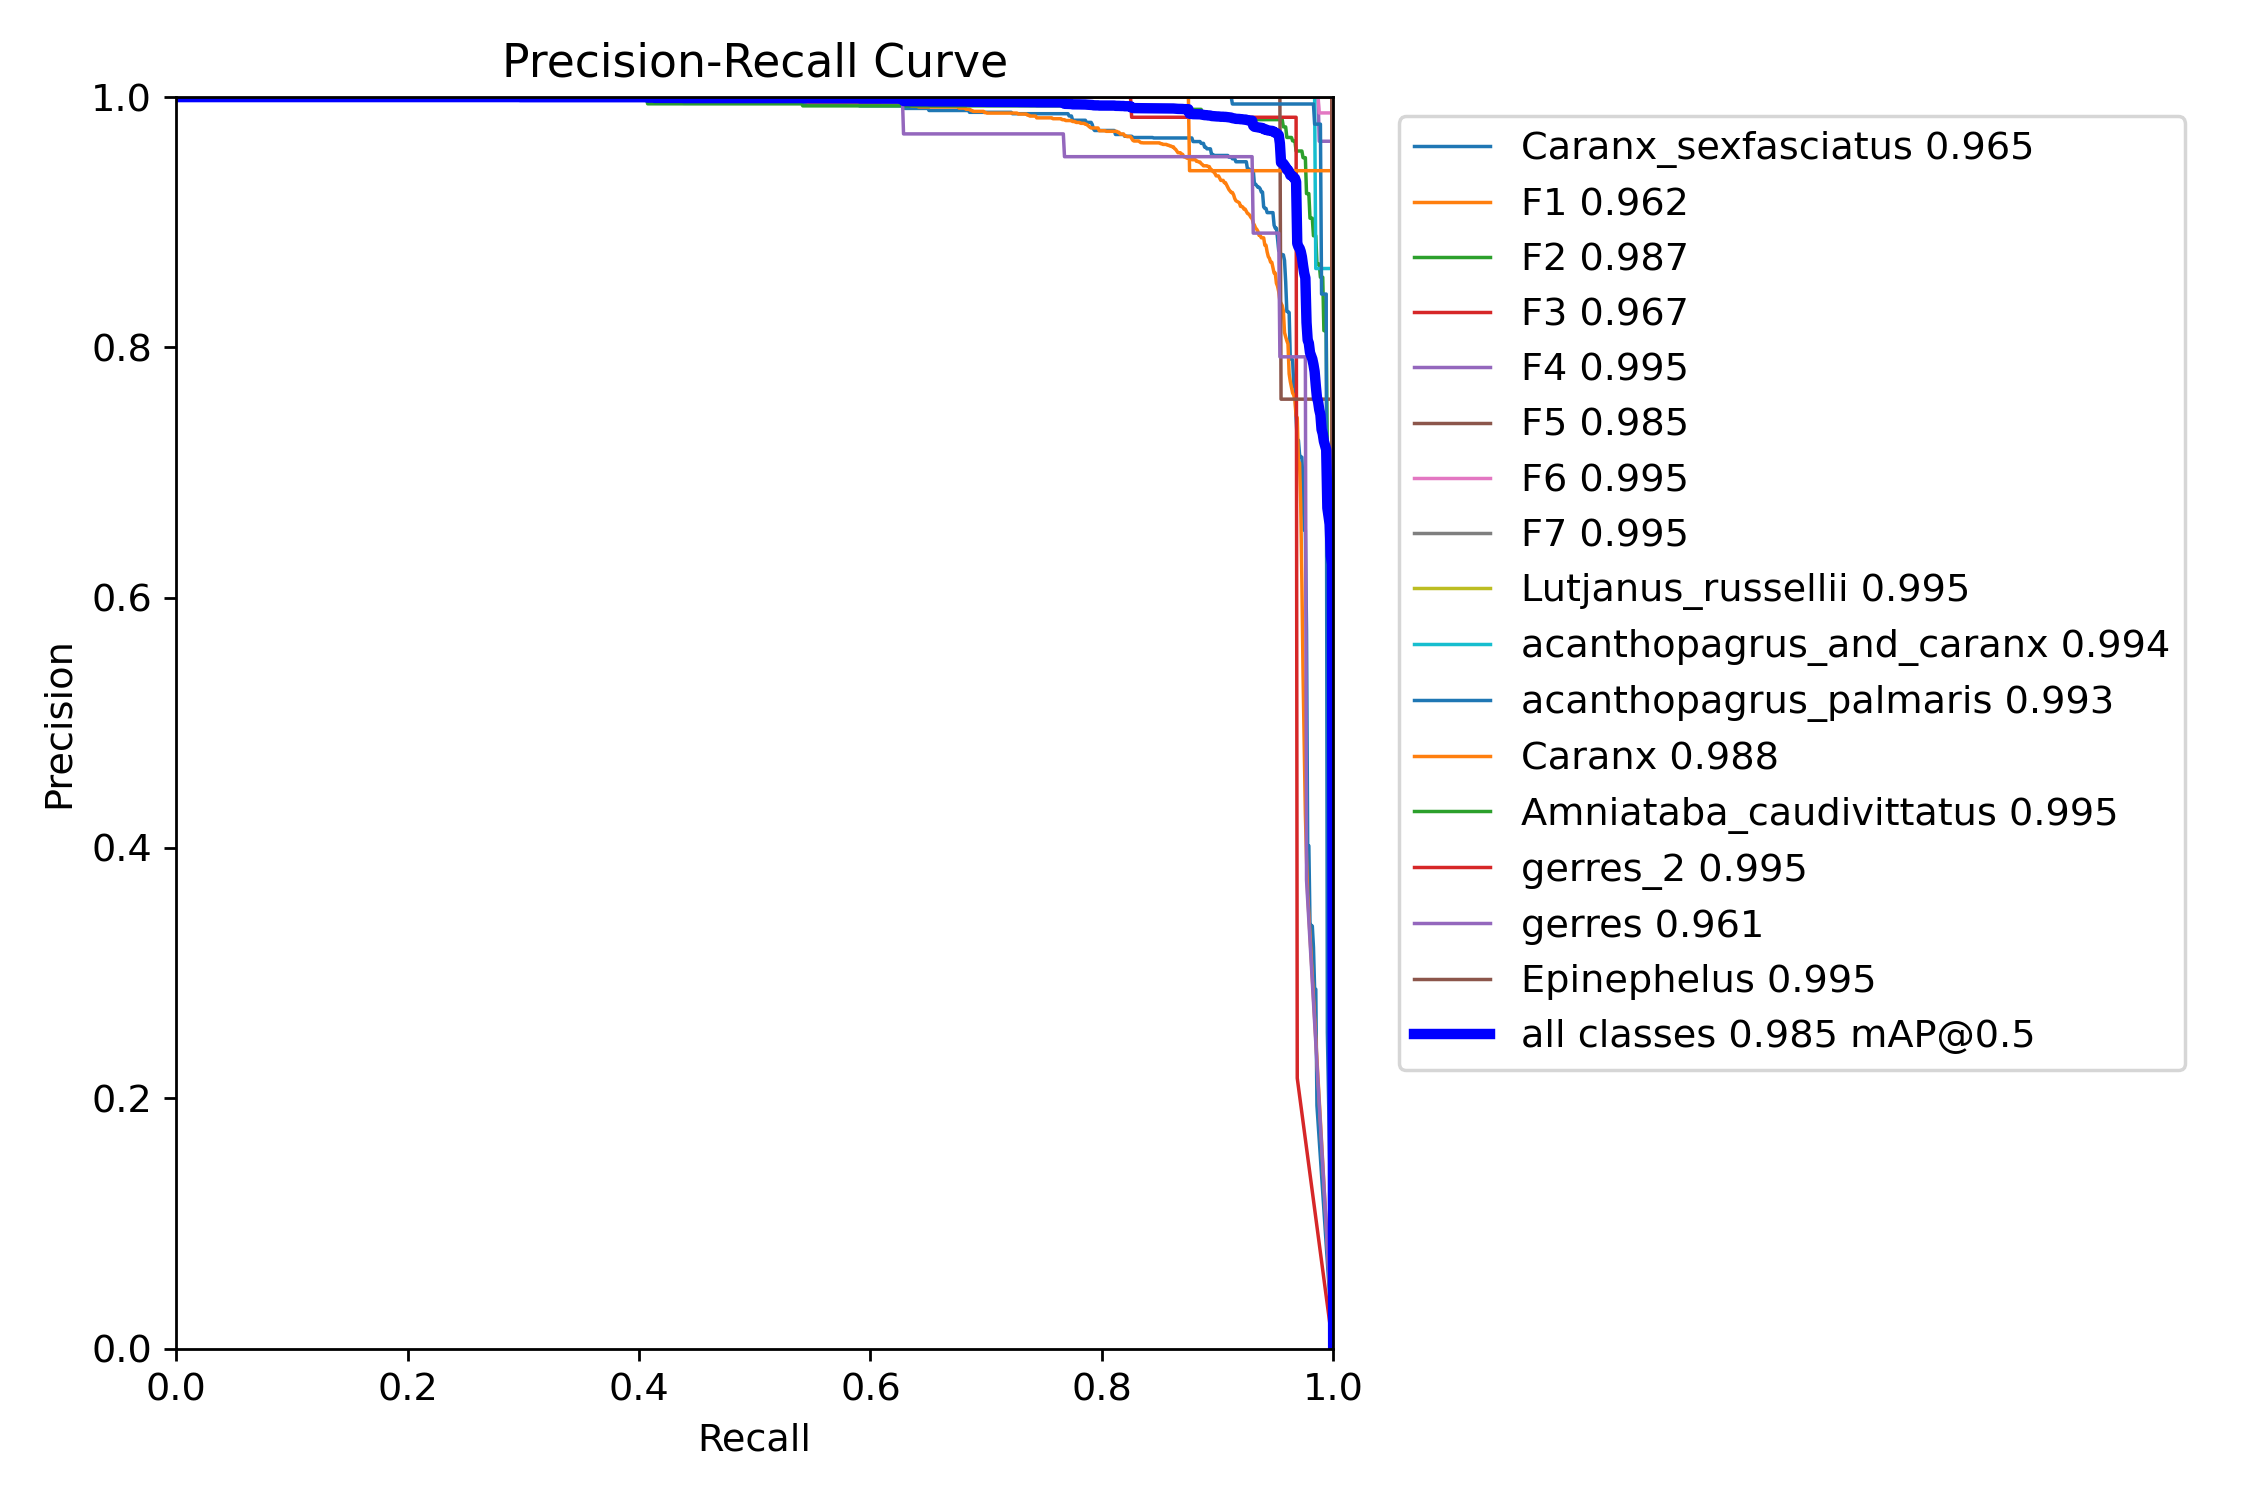
\includegraphics[width=\linewidth]{images/BoxPR_curve.png}
    \end{minipage}
    \hfill
    \begin{minipage}{0.49\linewidth}
        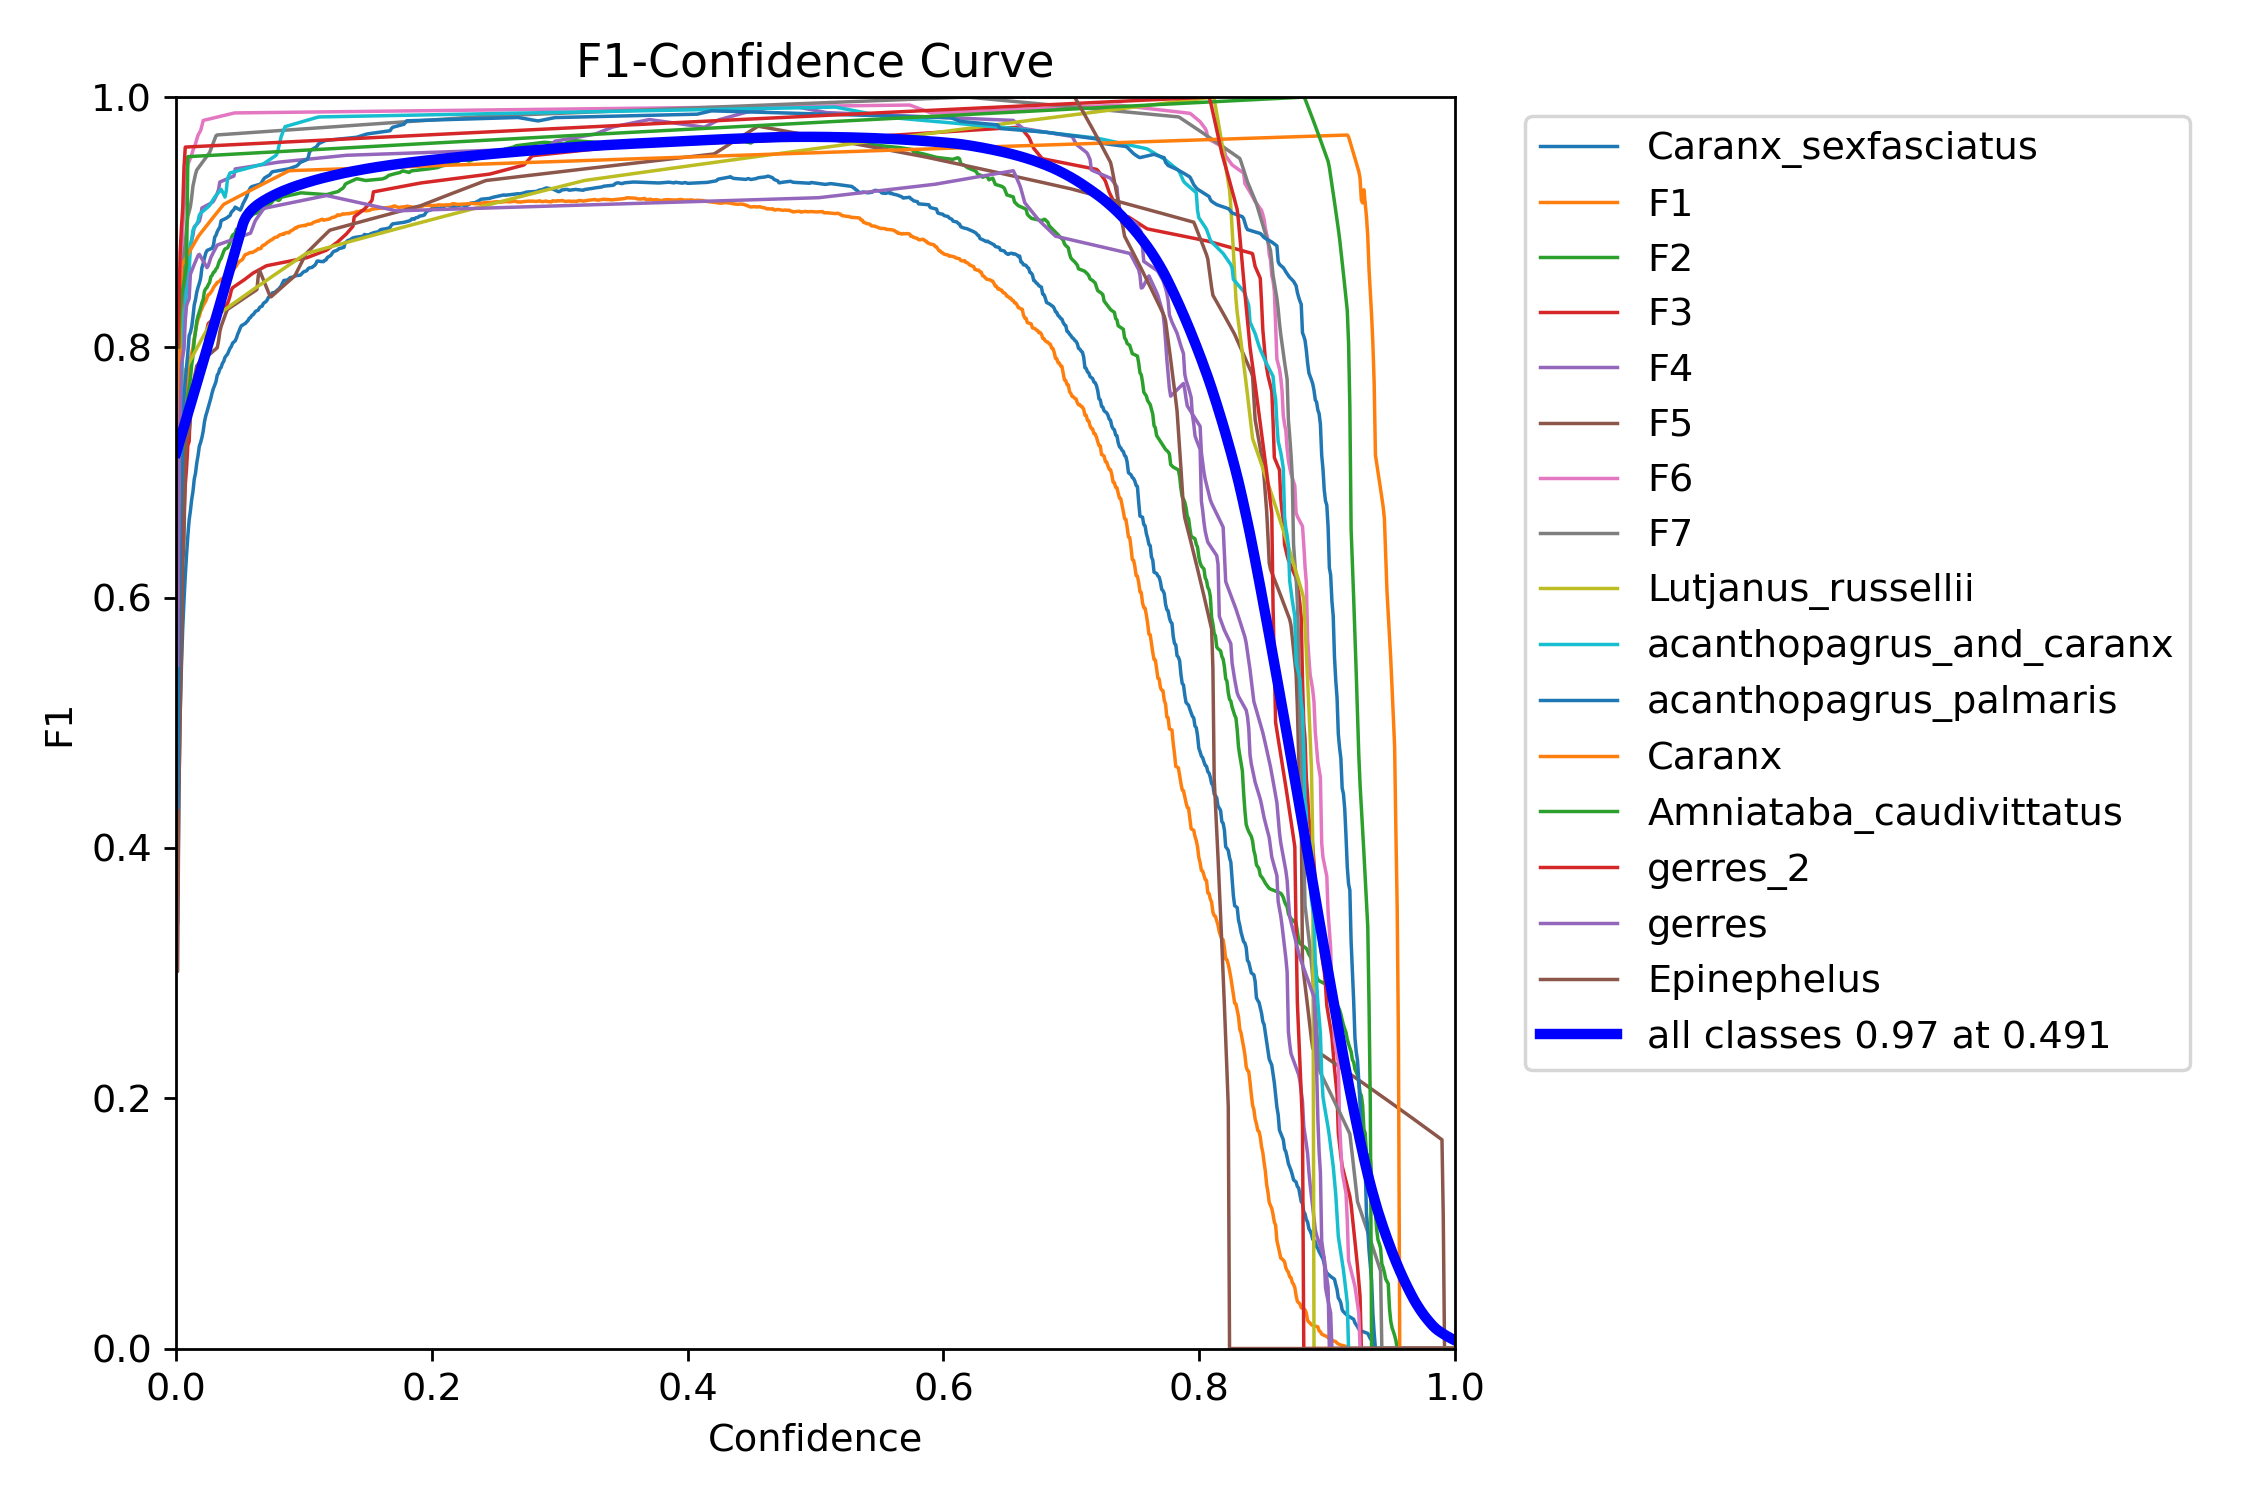
\includegraphics[width=\linewidth]{images/BoxF1_curve.png}
    \end{minipage}
    
\end{frame}


\begin{frame}{Fish Detection (DeepFish): Training Batch}

\begin{figure}
    \centering
    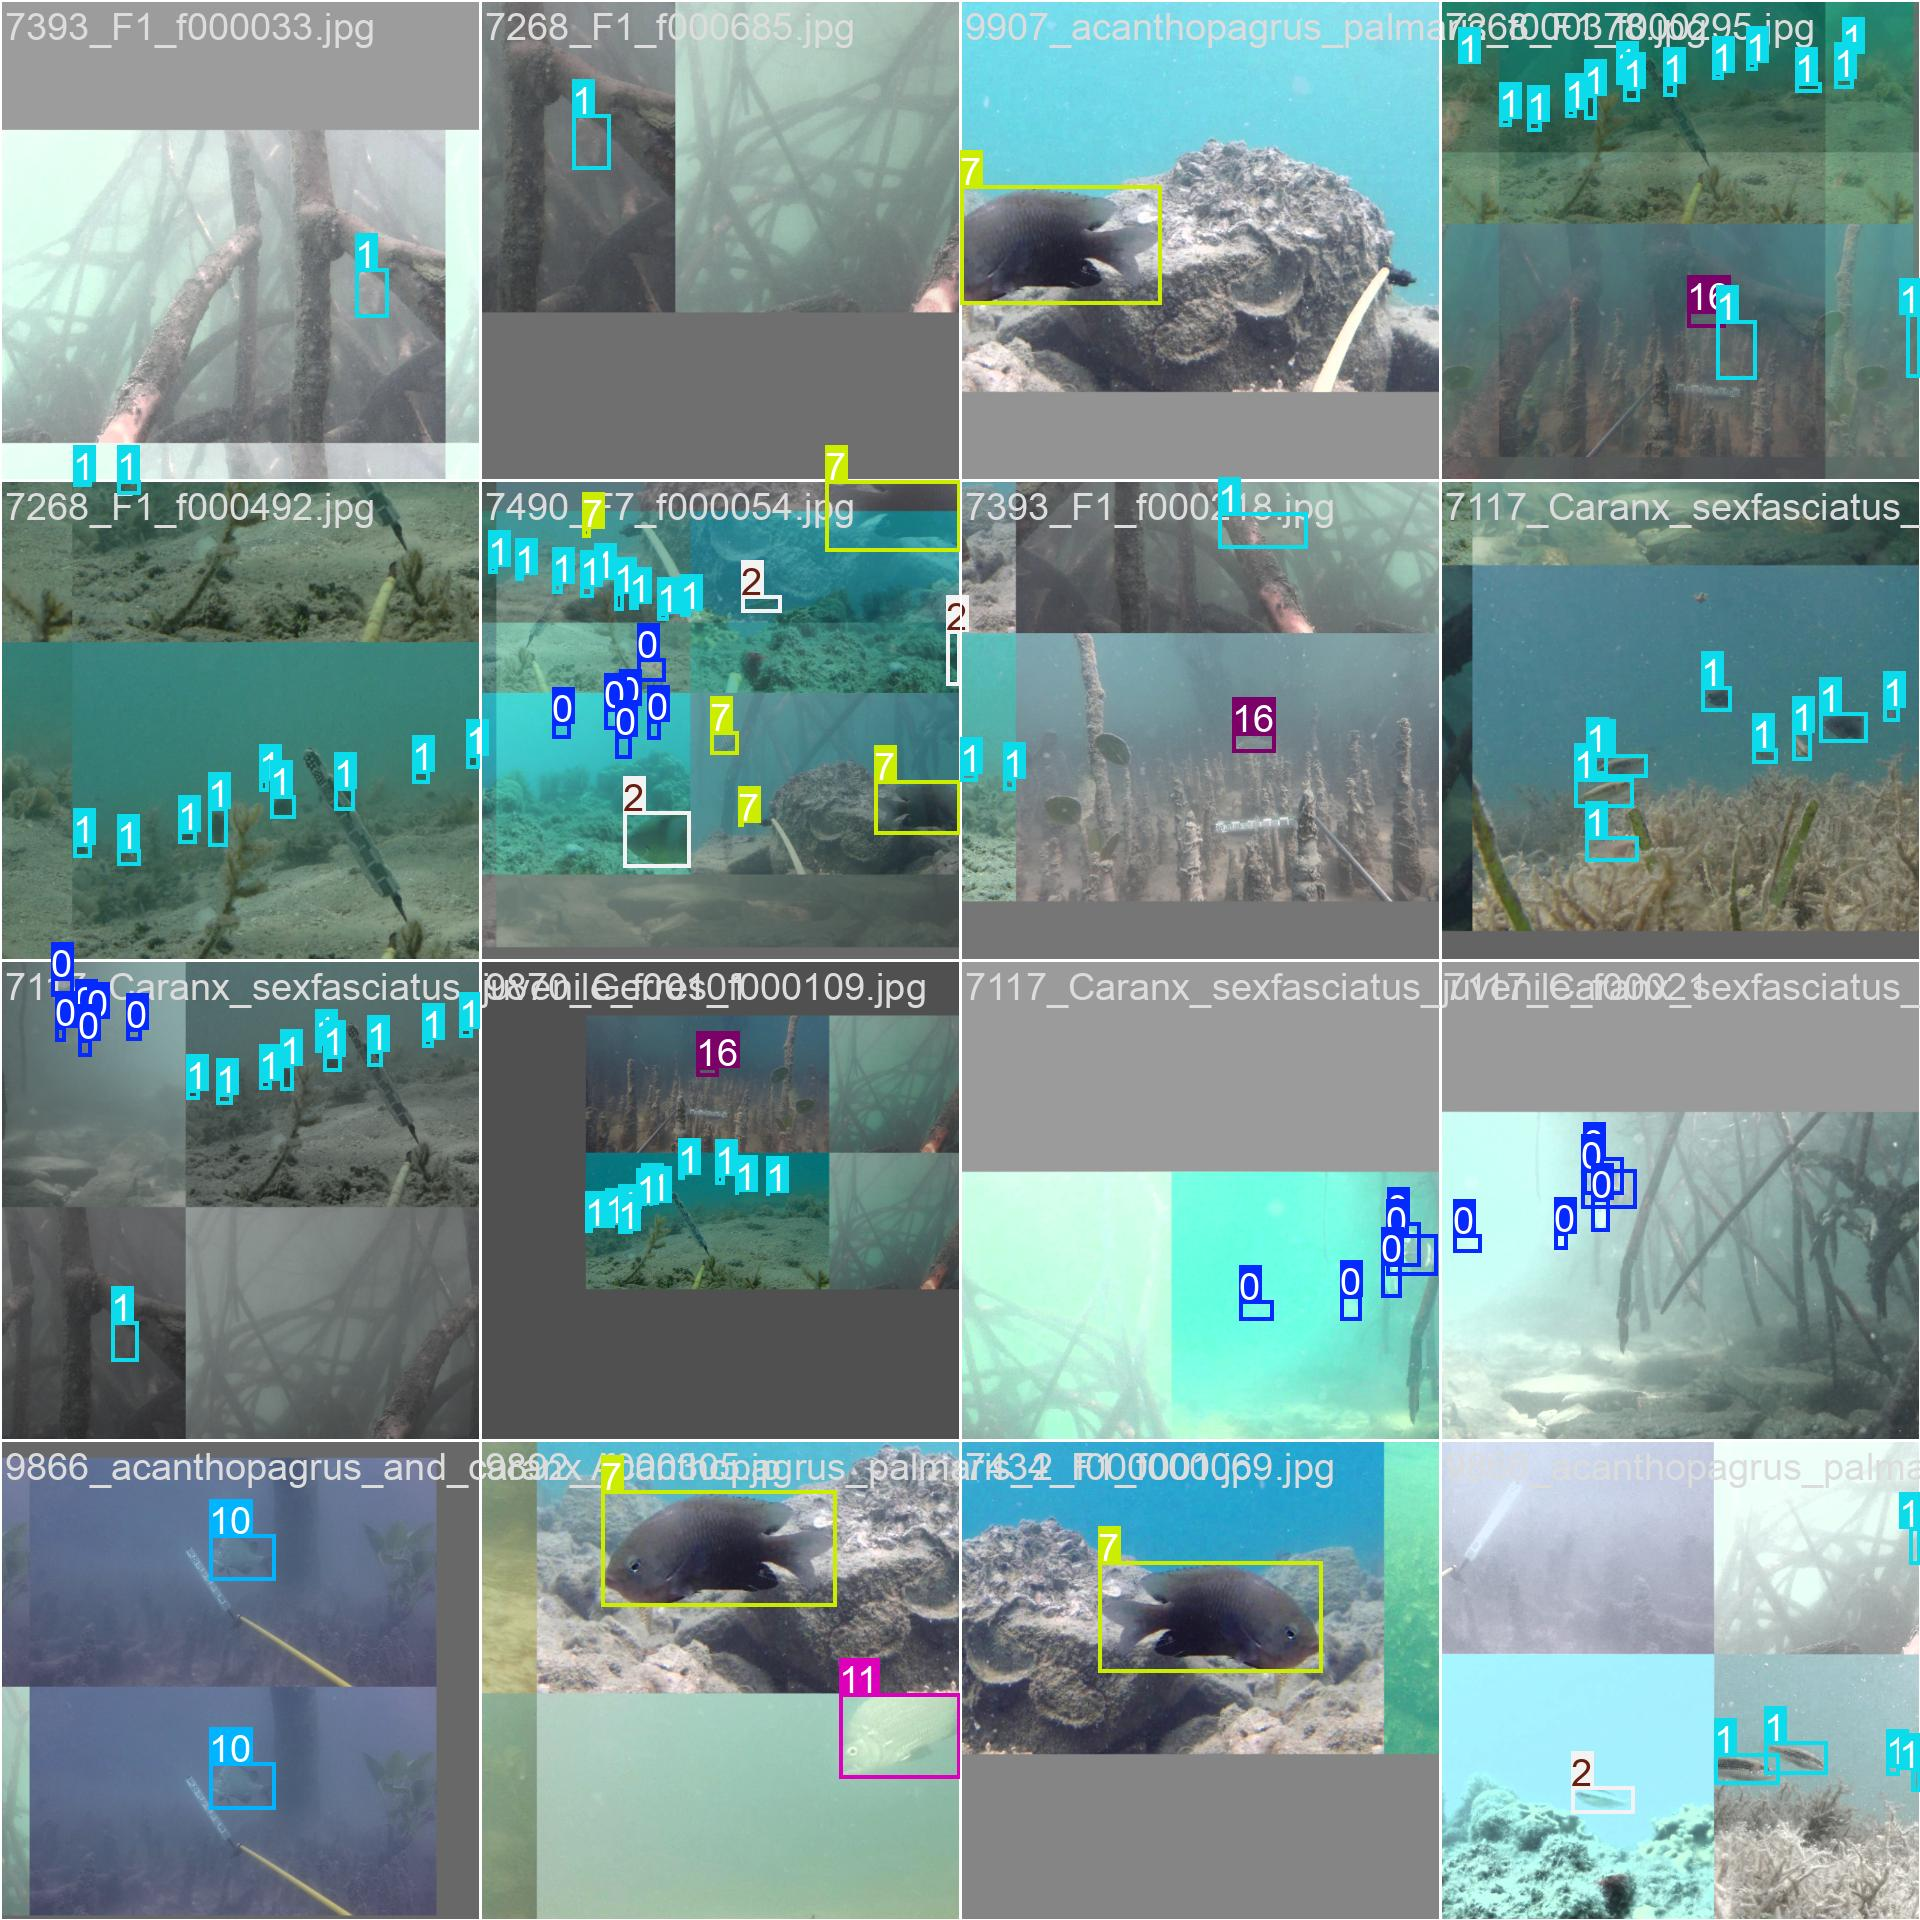
\includegraphics[width=0.60\linewidth]{images/train_batch2.jpg}
\end{figure}
    
\end{frame}


\begin{frame}{Fish Detection (DeepFish): Validation Batch}

\begin{figure}
    \centering
    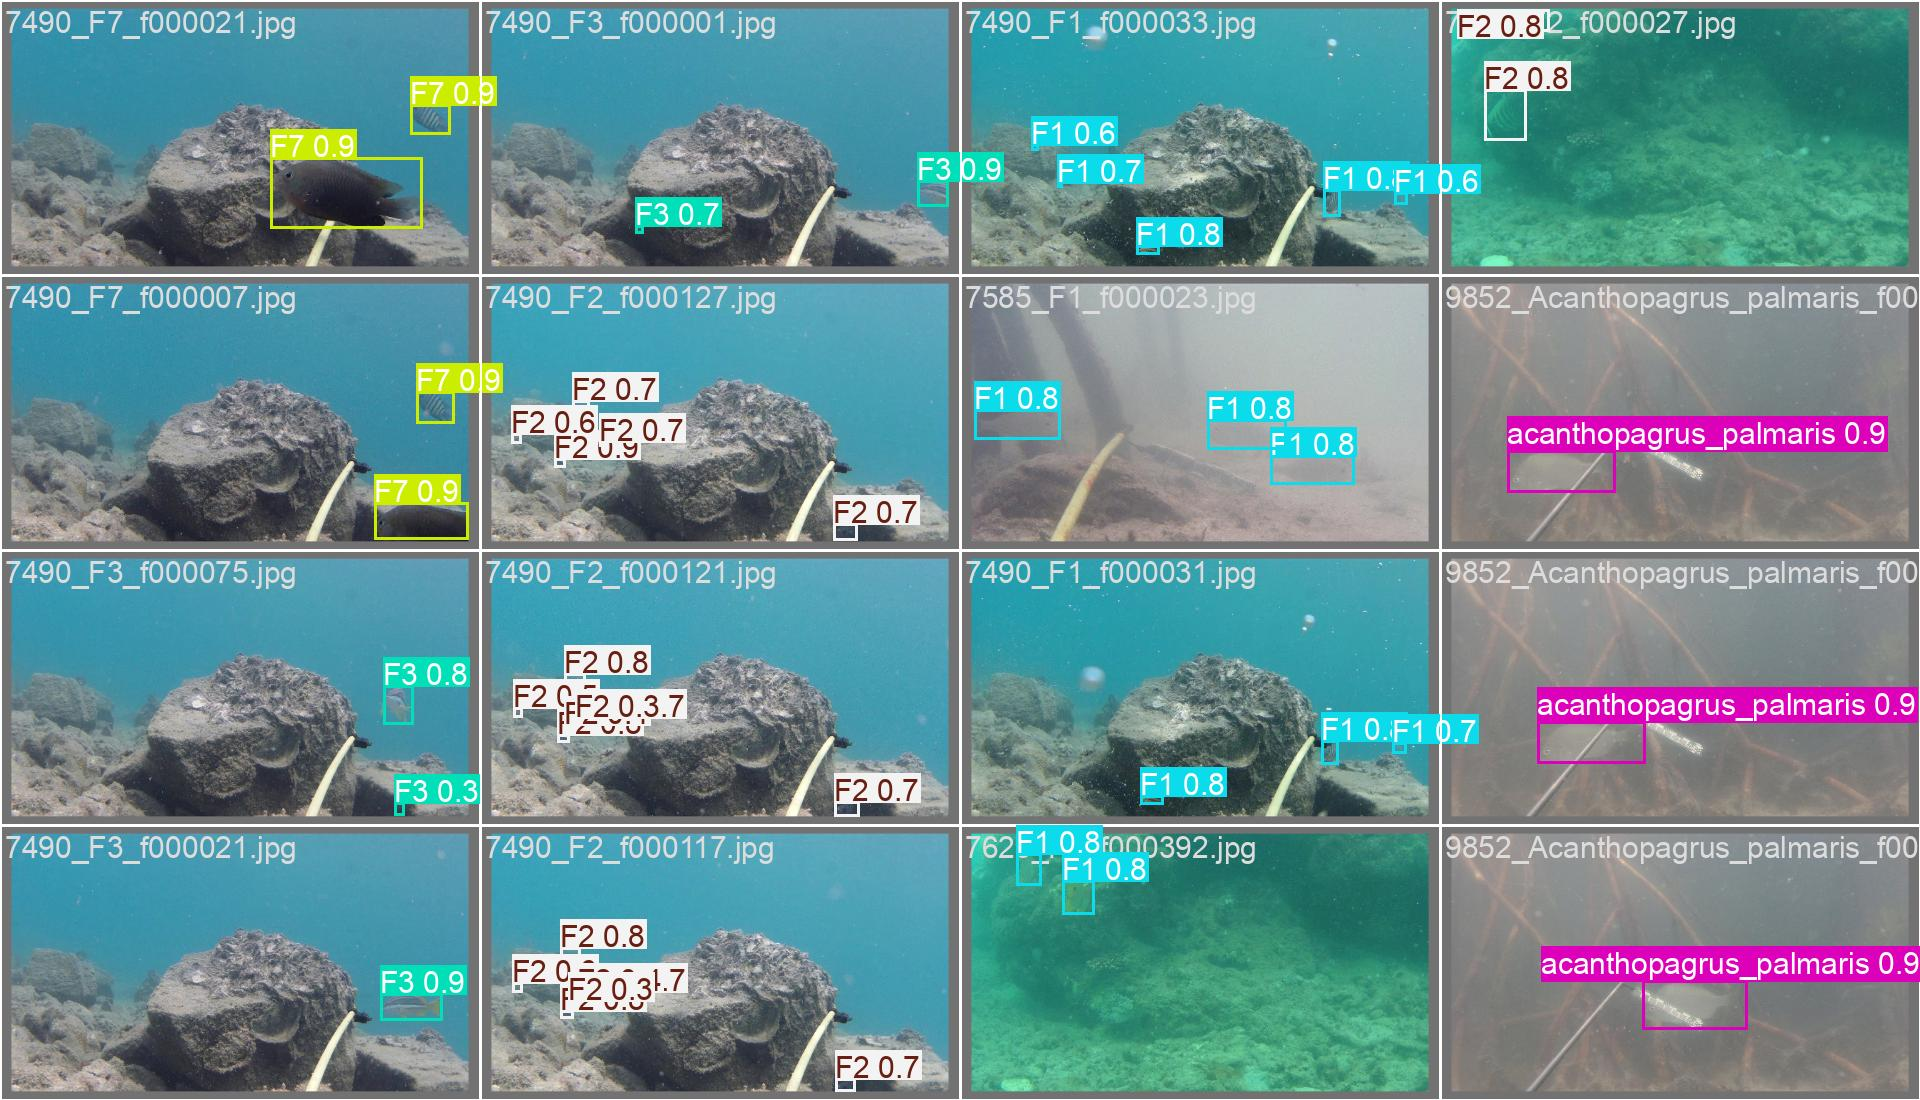
\includegraphics[width=0.8\linewidth]{images/val_batch1_pred.jpg}
\end{figure}
    
\end{frame}


\begin{frame}{Fish Tracking (F4K): Metrics}

\begin{figure}
    \centering
    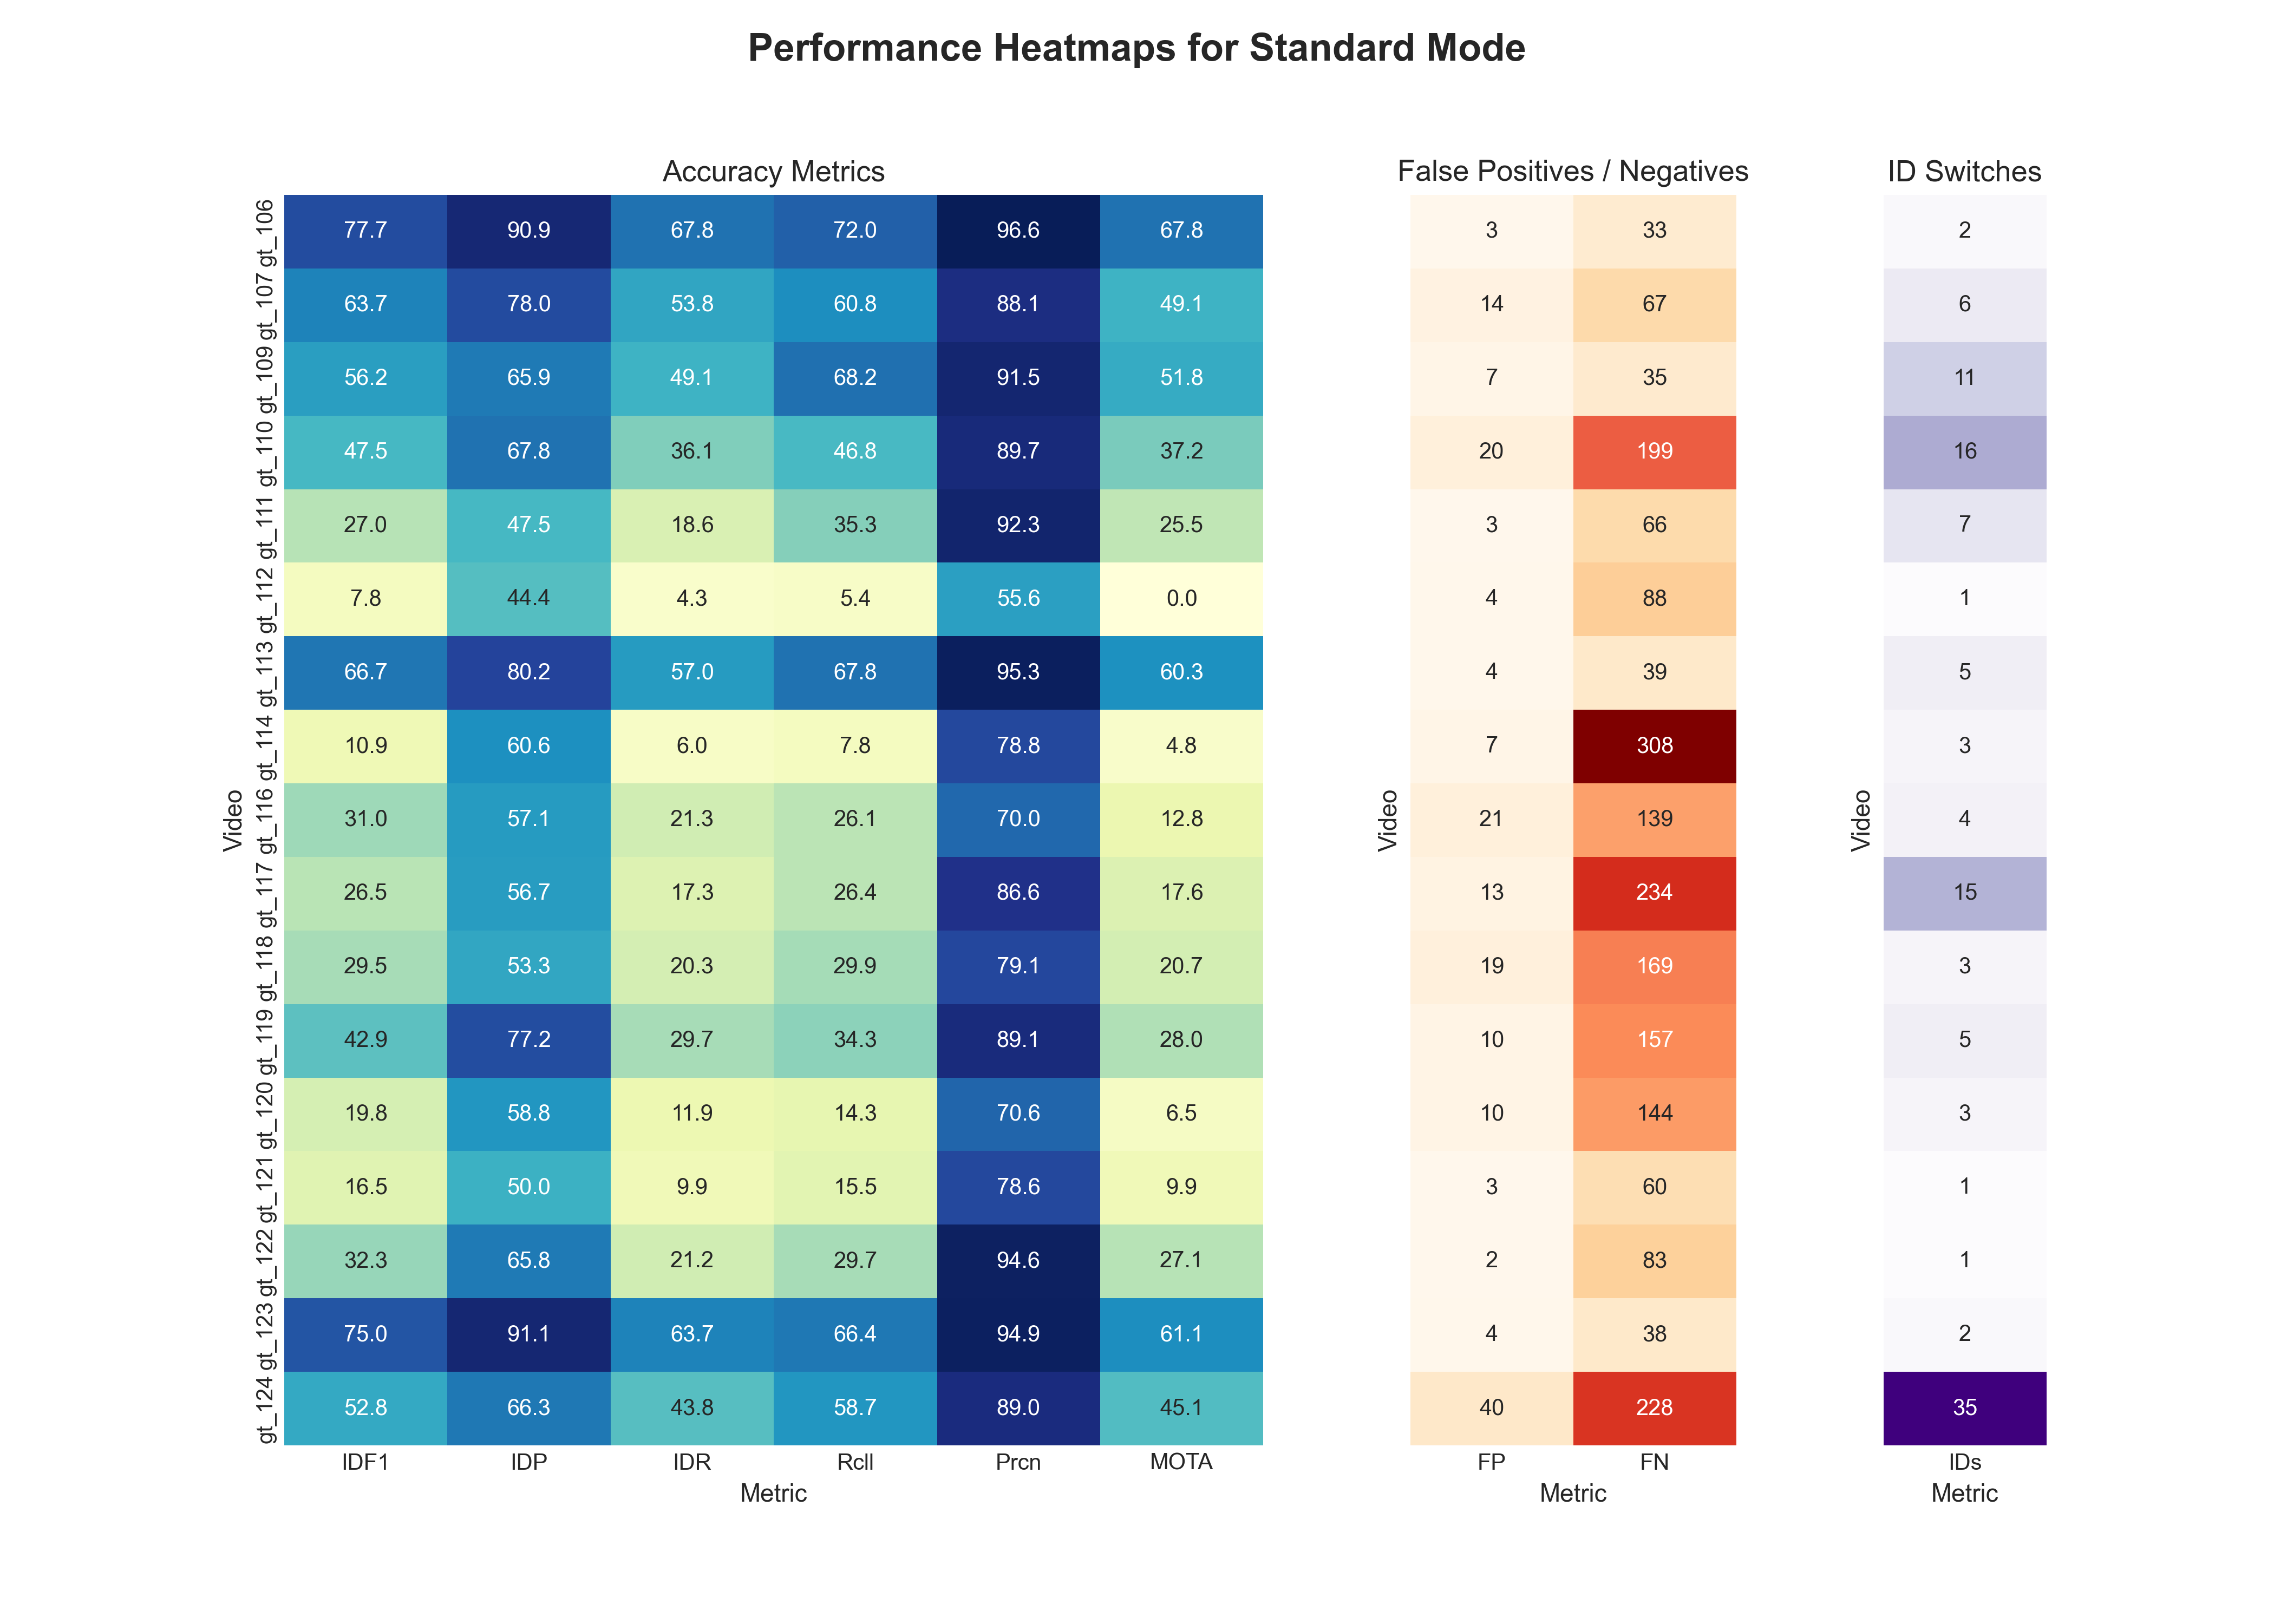
\includegraphics[width=\linewidth]{images/standard_performance_heatmap.png}
\end{figure}
    
\end{frame}






\section{Conclusions}

\begin{frame}{Conclusions}
    Successful pipeline for real-time fish detection, tracking, and classification.
    \vspace{1.5em}
    \begin{figure}
        \centering
        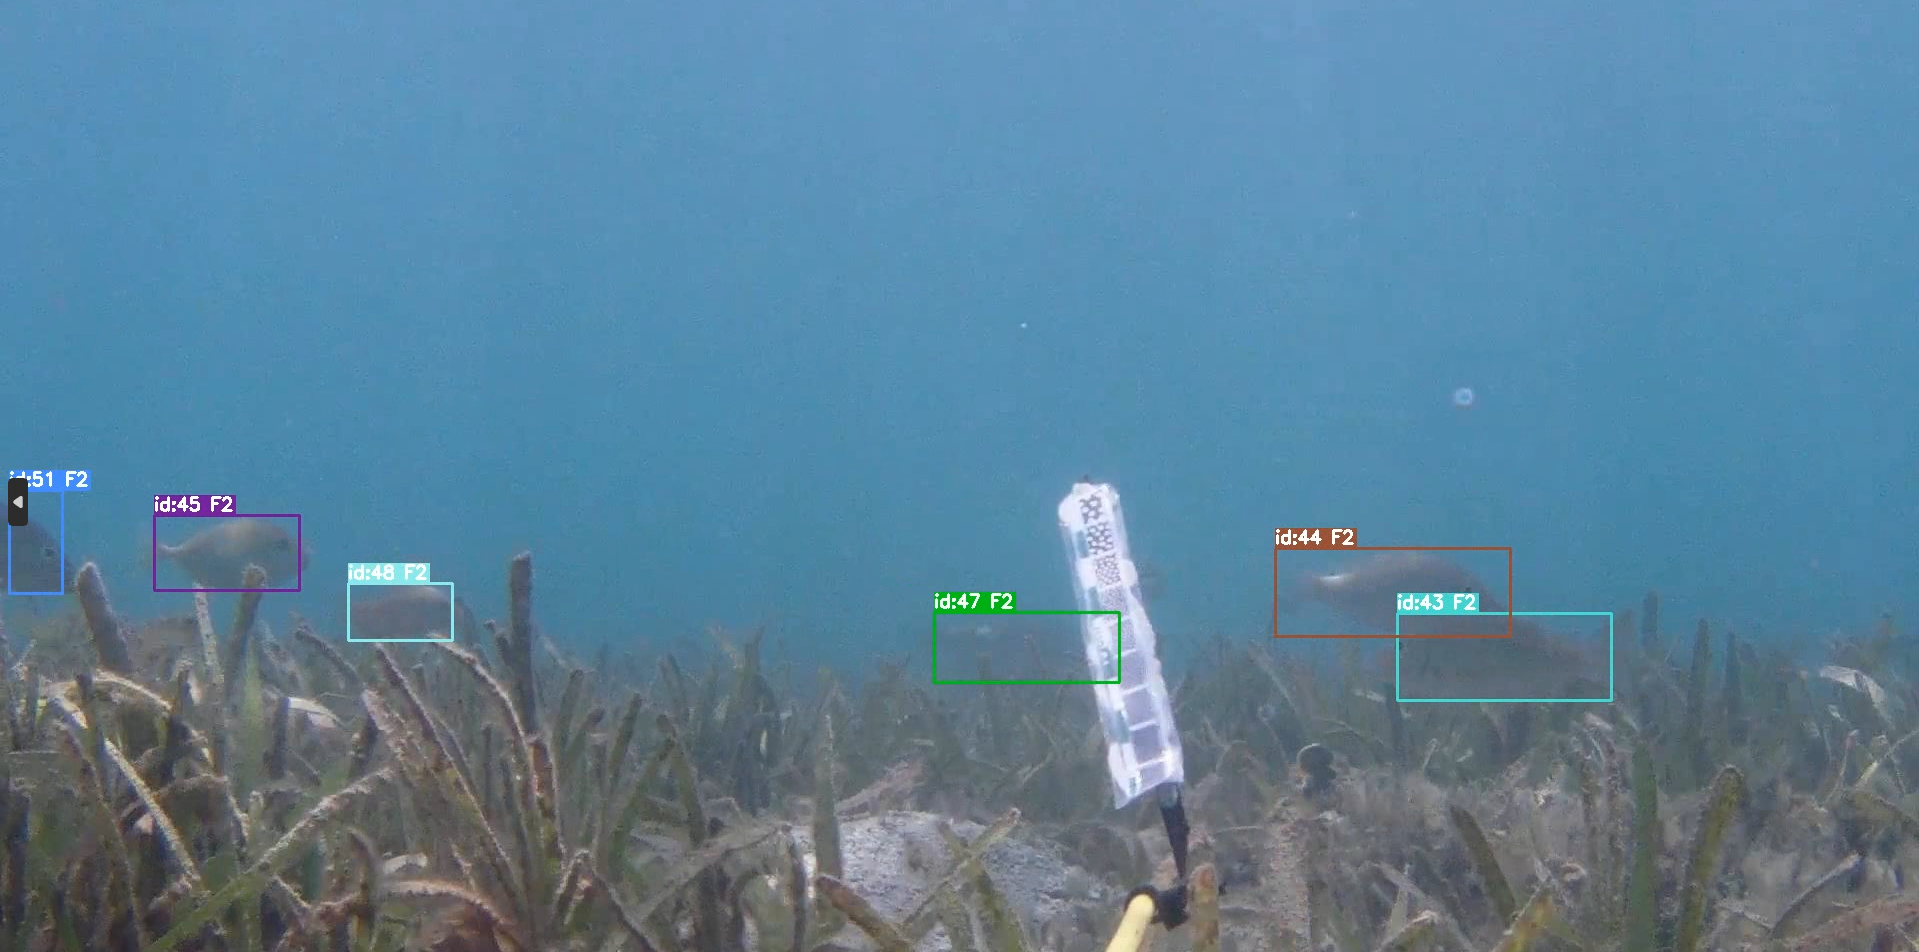
\includegraphics[width=0.8\linewidth]{images/video_screenshot.png}
    \end{figure}

\end{frame}


\begin{frame}{Future Work}
    
    \vspace{1.5em}
    
    \begin{columns}[T,totalwidth=\textwidth]
        
        \begin{column}{0.32\textwidth}
            \centering
            \includegraphics[width=0.6\linewidth]{images/brain_icon.jpg}
            \vspace{1em}
            \parbox{\linewidth}{\centering\textbf{\\Improve Detector Robustness}}
        \end{column}
        
        \begin{column}{0.32\textwidth}
            \centering
            
\includegraphics[width=0.6\linewidth]{images/video_icon.jpg}
            \vspace{1em}
            \parbox{\linewidth}{\centering\textbf{\\Deploy on Video Devices}}
        \end{column}
        
        \begin{column}{0.32\textwidth}
            \centering
            \vspace{1em}
            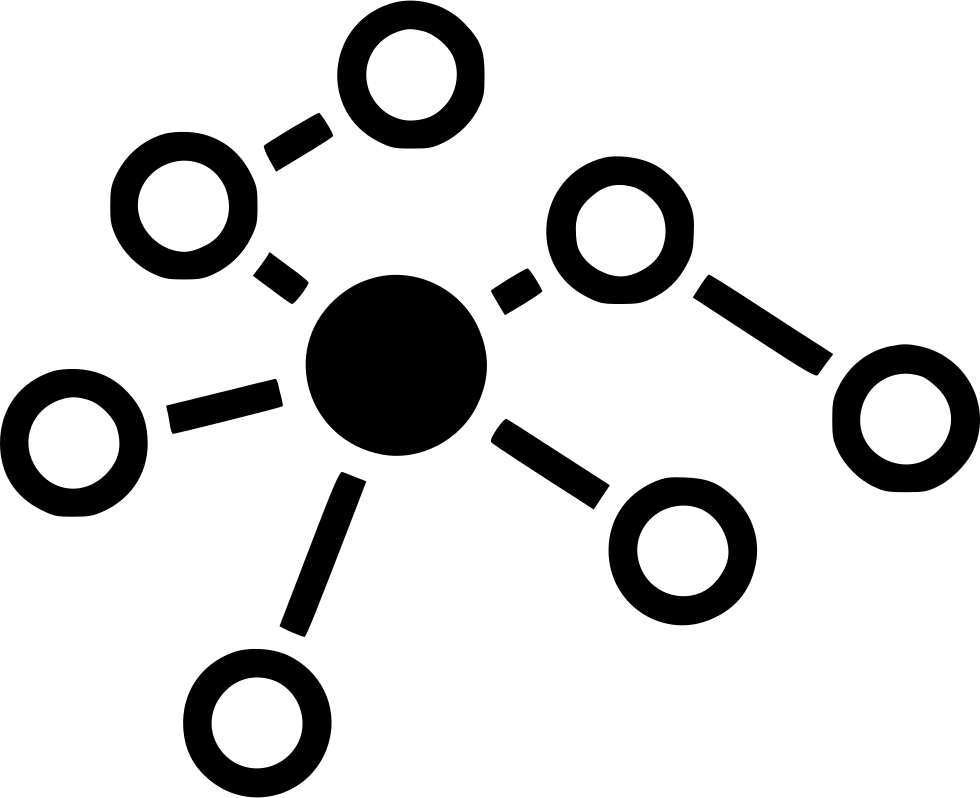
\includegraphics[width=0.6\linewidth]{images/graph_icon.png}
            \vspace{1em}
            \parbox{\linewidth}{\centering\textbf{\\Enable Behavioral Analysis}}
        \end{column}
        
    \end{columns}
    
\end{frame}

\begin{frame}
\centering
{\Huge Thank you!}
\end{frame}

\begin{frame}
    \centering
    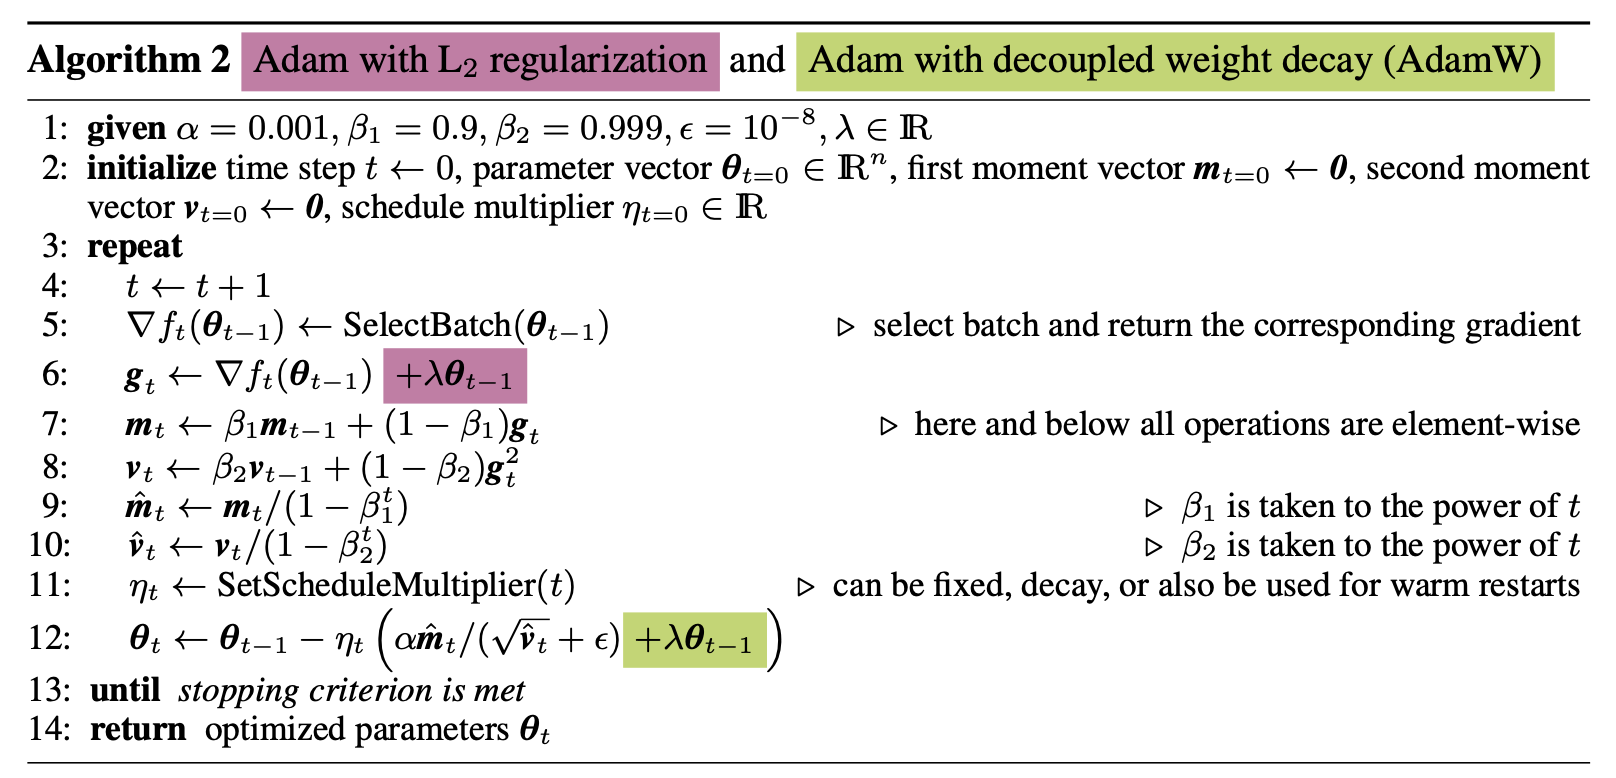
\includegraphics[width=\textwidth]{images/adamw_algo.png}
    \footnote{\cite{loshchilov2019decoupledweightdecayregularization}}
    \end{frame}
    
    \begin{frame}
    \centering
    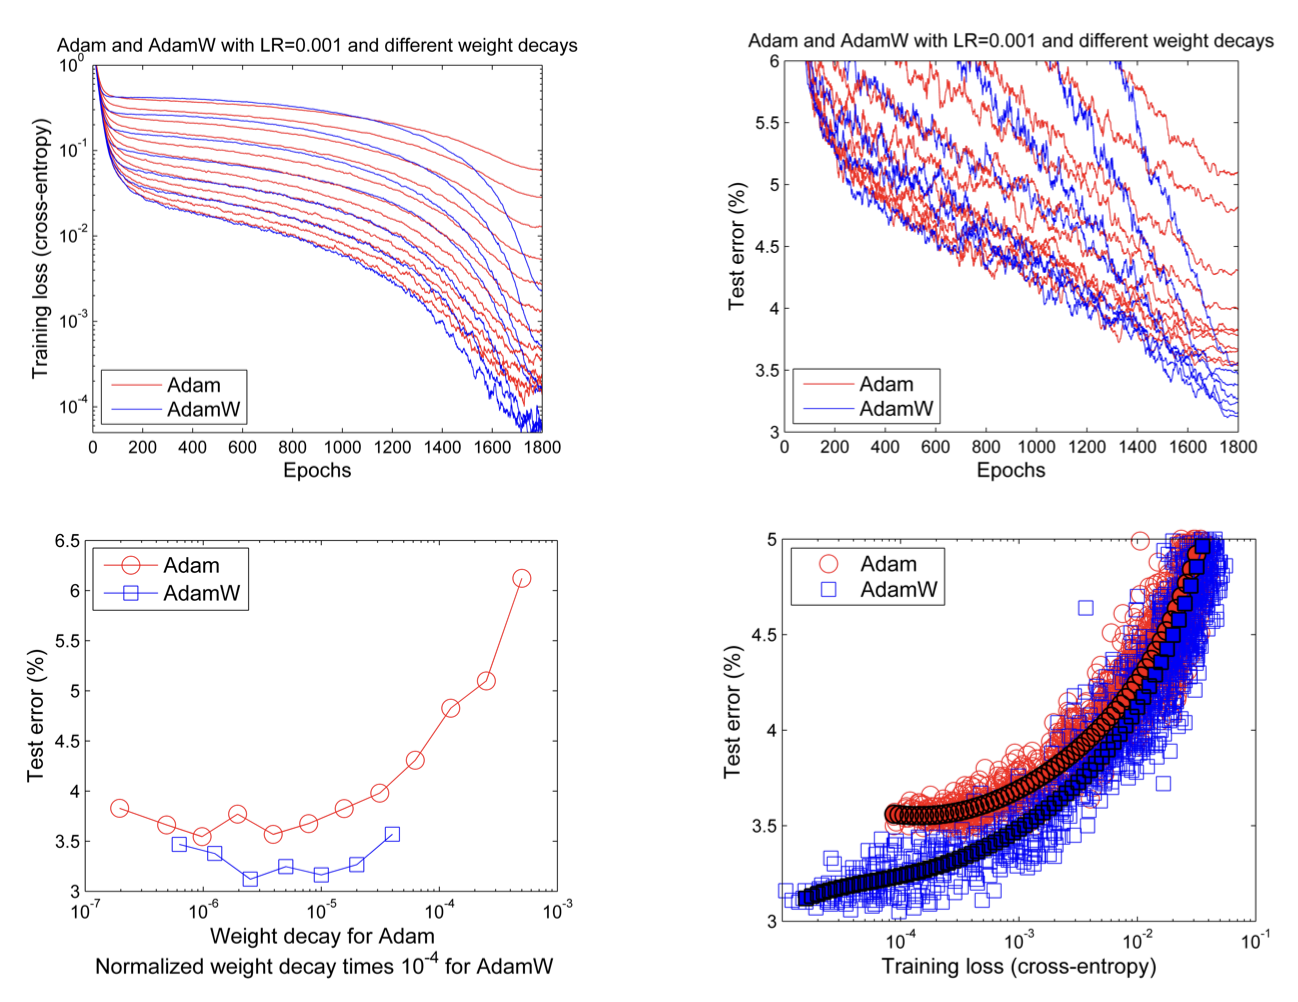
\includegraphics[width=0.8\textwidth]{images/adamw_com.png}
    \footnote{\cite{loshchilov2019decoupledweightdecayregularization}}
    \end{frame}

{\tiny
\bibliography{ref}
\bibliographystyle{plain}
}

\end{document}
